% ============================================================================
% Paper 3 -- integrated from papers/meds_owl_JBI_2(1)/main.tex and supplementary.tex (front matter transcribed
% from the cas-dc \title/\author/\affiliation/\credit, abstract, graphical abstract and keywords; body converted
% mechanically, see the integration report). No bibliographic record for this paper was supplied, so it is not
% cited here.
% ============================================================================
\section{MEDS-OWL: An Ontology-Driven Framework for Clinical Outcome Prediction with Graph Learning}
\label{sec:paper3}

\paragraph{Authors.}
Alberto Marfoglia\textsuperscript{1,2,*}, Antonella Carbonaro\textsuperscript{1,*}, Adrien Coulet\textsuperscript{2,*}

{\raggedright % layout: ragged-right metadata block
\noindent\textsuperscript{1}Dept.\ of Computer Science and Engineering (DISI), University of Bologna, Bologna, Italy\\
\textsuperscript{2}Inria, Inserm, Universit\'e Paris Cit\'e, HeKA, UMR 1346, Paris, France\\
\textsuperscript{*}Corresponding author.\\
E-mail addresses: alberto.marfoglia2@unibo.it (A. Marfoglia), antonella.carbonaro@unibo.it (A. Carbonaro), adrien.coulet@inria.fr (A. Coulet).\\
URLs: \url{https://albertomarfoglia.github.io/} (A. Marfoglia), \url{https://www.unibo.it/sitoweb/antonella.carbonaro} (A. Carbonaro), \url{https://heka.gitlabpages.inria.fr/team/members/coulet.html} (A. Coulet).\\
ORCID: 0009-0000-5857-2376 (A. Marfoglia), 0000-0002-3890-4852 (A. Carbonaro), 0000-0002-1466-062X (A. Coulet).
\par}

{\raggedright
\noindent\textsuperscript{a}Dept. of Computer Science and Engineering (DISI), University of Bologna, Bologna, Italy\\
\textsuperscript{b}Inria, Inserm, Universit\'e Paris Cit\'e, HeKA, UMR 1346, Paris, France\\
\textsuperscript{*}Corresponding authors.\\
Preprint submitted for publication in the Journal of Biomedical Informatics. Available at SSRN: \url{https://papers.ssrn.com/sol3/papers.cfm?abstract_id=7545256}.\\
\par}

\subsection*{Abstract}

Objective: To develop a formal semantic representation of the Medical Event Data Standard (MEDS), an event-centric standard for structured clinical data, using Semantic Web technologies and supporting reproducible graph-based machine learning. We further investigate how the semantic granularity of the resulting graph representation affects clinical outcome prediction.\\
Methods: We present MEDS-OWL, a lightweight ontology that extends MEDS with a formal semantic representation, together with \texttt{meds2rdf}, a scalable Python library for transforming MEDS-compliant datasets into FAIR-aligned MEDS-RDF graphs. Round-trip fidelity and scalability were evaluated on four heterogeneous clinical datasets (NEUROVASC, MIMIC-IV, eICU, and NWICU), comprising more than 309,000 hospital stays. For downstream evaluation, 11 prediction tasks derived from MIMIC-IV were formulated as patient-level binary classification problems. A two-layer Relational Graph Convolutional Network with literal-aware encoding was evaluated across three MEDS-RDF schema variants differing in subject–event predicate granularity, enabling systematic assessment of the influence of representation granularity on graph-based learning.\\
Results: The framework preserved structural completeness and the core MEDS fields with high fidelity across the four datasets. Its streaming conversion architecture enabled processing RDF graphs of up to 937 GB, achieving a 2.7$\times$ speedup over its predecessor. Across the 11 prediction tasks, increasing semantic granularity from MEDS-RDF-Base to Partial to Full consistently improved Macro-F1, narrowing the performance gap with tabular baselines.\\
Conclusions: MEDS-OWL provides a scalable, interoperable, and FAIR-aligned framework for representing MEDS data as semantic clinical graphs. The results demonstrate that semantic representation extends beyond interoperability and therefore should be treated as an important determinant of graph-based clinical machine learning performance in predictive analytics for clinical outcomes.

\subsection*{Graphical abstract}

\begin{center}
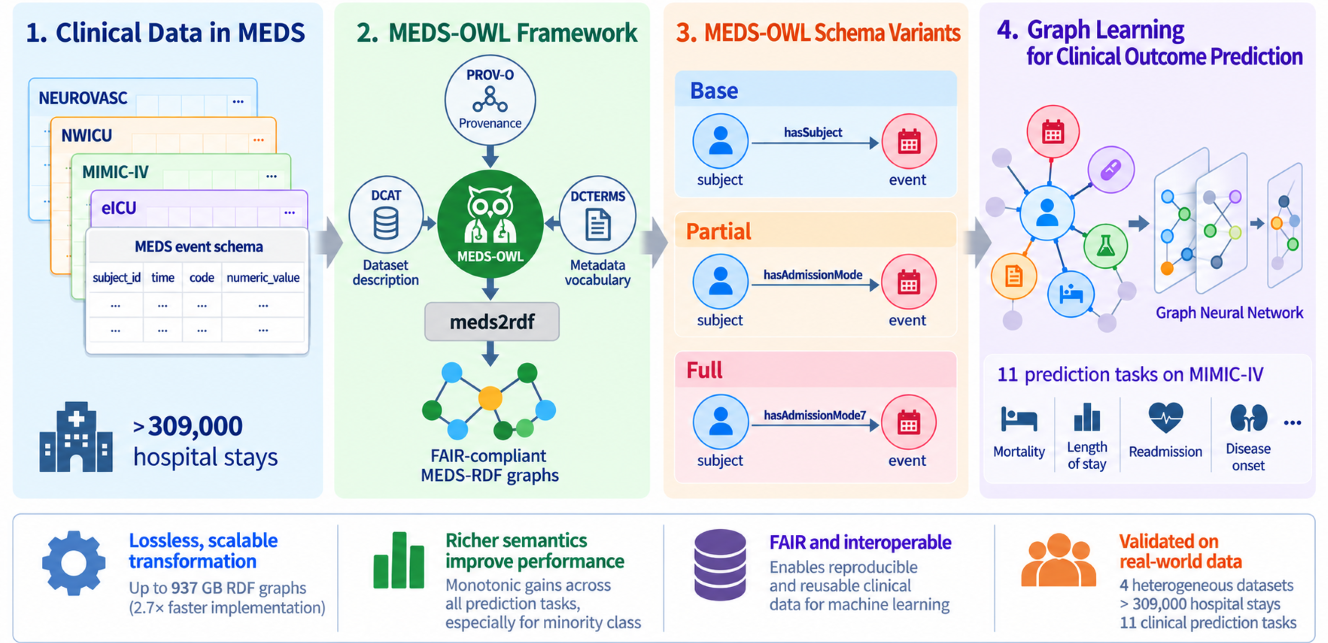
\includegraphics[width=\textwidth]{figures/paper3/graphical_abstract.png}
\end{center}

\paragraph{Keywords:} Medical Event Data Standard (MEDS); Knowledge graph; OWL ontology; Graph Convolutional Network; Healthcare; Predictive machine learning; FAIR principles

\subsection{Introduction}
Machine learning (ML) in healthcare is hindered by the lack of standardized representations for structured Electronic Health Record (EHR) data, resulting in dataset-specific preprocessing practices, limited reproducibility, and poor model portability across datasets. The Medical Event Data Standard (MEDS)~\cite{bert_arnrich_medical_2024,mcdermott_meds_2024} addresses this gap by introducing a unified, event-centric schema for longitudinal health data that is explicitly designed to support reproducible and efficient ML workflows. MEDS represents each clinical event using a minimal tuple consisting of a subject identifier, a code, and optional temporal and value attributes. This lightweight and pragmatically oriented design makes MEDS suitable for benchmarking, multi-center studies, and the development of foundation models. Accordingly, MEDS has been adopted in several ML projects; for example, it has been used to train transformer-based models for predicting future events in patient healthcare trajectories~\cite{renc_foundation_2025,oufattole_meds-tab_2024}.

In its native form, MEDS is a data-format specification and does not provide ontology-level semantics. The Semantic Web paradigm offers a complementary approach to address this limitation~\cite{hitzler_foundations_2009,MARFOGLIA2026108380}. Ontologies expressed using Resource Description Framework (RDF) and Web Ontology Language (OWL) provide machine-interpretable and interoperable representations of entities and their relationships, while supporting semantic querying and formal reasoning. They also enable the construction of knowledge graphs (KGs), facilitating the explicit linkage of dataset elements to external terminologies such as LOINC, SNOMED CT, or ATC~\cite{hogan_knowledge_2021}. 

Projecting MEDS datasets into RDF would thus facilitate their semantic integration and validation while creating opportunities for graph-based ML on longitudinal clinical data. By explicitly representing subjects, events, and their relationships as a graph, such representations can be processed using ML methods that exploit relational structure\cite{schlichtkrull_2018}. Despite the growing use of clinical KGs and graph neural networks, the effect of semantic representation granularity on graph-based clinical prediction has received limited systematic investigation.

In this study, we propose a semantic framework for representing MEDS-based clinical data as interoperable and FAIR-aligned graphs. This work is the first to (i) formalize a general-purpose OWL ontology named MEDS-OWL for the MEDS standard, (ii) develop a scalable, streaming MEDS-RDF conversion library validated at production scale, named \texttt{meds2rdf}, and (iii) demonstrate the utility of the MEDS-OWL representation for clinical outcome prediction on real-world data by systematically varying predicate granularity as an independent variable in graph-based predictive modeling.

\begin{table}[htbp]
\centering
\begin{tabular}{p{0.2\textwidth} p{0.8\textwidth}}
\hline
\textbf{Problem or Issue} &
MEDS provides a standardized event-centric format for clinical data, but lacks ontology-level semantics, limiting semantic interoperability and leaving the effect of representation granularity on graph-based prediction unclear.
\\[0.5em]

\textbf{What is Already Known} &
RDF and clinical knowledge graphs support interoperability, provenance, semantic querying, and graph-based learning, but existing representations are often tailored to specific data models, infrastructures, or use cases.
\\[0.5em]

\textbf{What this Paper Adds} &
We introduce MEDS-OWL, a general-purpose OWL ontology for MEDS, and meds2rdf, a scalable streaming framework for generating FAIR MEDS-RDF graphs. We further systematically evaluate how subject-event predicate granularity affects graph-based clinical outcome prediction across 11 MIMIC-IV tasks.
\\[0.5em]

\textbf{Who would benefit from the new knowledge in this paper} &
Clinical informatics researchers, biomedical data scientists, and machine-learning researchers working with interoperable, reproducible graph representations of longitudinal clinical data.
\\
\hline
\end{tabular}
\end{table}
%
%
%
%
%

\subsection{Related Work}
\label{sec:paper3_related_work}
%
While several data models and ontologies, such as FHIR~\cite{lehne_use_2019}, OMOP CDM~\cite{xiao_fhir-ontop-omop_2022}, and Phenopackets~\cite{kaliyaperumal_phenopackets_2022}, have been proposed to harmonize clinical data, RDF transformations of these models have seen limited adoption~\cite{xiao_fhir-ontop-omop_2022,marfoglia_towards_2025}, in part due to loosely specified semantics or incomplete coverage of the clinical domain.
Patient-centric RDF-based representations such as SPHN~\cite{toure2023} and CARE-SM~\cite{kaliyaperumal_semantic_2022} illustrate how KGs can facilitate interoperability, provenance modeling, and temporal reasoning.
However, these models are often tightly coupled to specific use cases or semantic frameworks.

KGs provide a natural representation for clinical data in which patients, events, concepts, and their relationships can be represented explicitly. KG embeddings map graph nodes and edges into continuous vector spaces, enabling relational structures to be incorporated into computational models~\cite{hamilton_representation_2018}. Such representations have been applied to tasks including link prediction, node classification, and clustering~\cite{wang_knowledge_2017}. Graph neural networks extend these ideas by learning representations directly from graph structure. In particular, Relational Graph Convolutional Networks (RGCNs) have been shown good performances when the underlying schema aligns with task-specific requirements~\cite{schlichtkrull_2018}; for instance, compact and patient-centered representations for outcome prediction \cite{MARFOGLIA2026108380}. 

MEDS-OWL addresses these gaps by providing a semantic representation of a data model specifically designed for ML research in healthcare. It preserves the compact, event-centric design of MEDS while adding ontology-level semantics, combining representation compactness with semantic expressiveness. This positions MEDS-OWL as a semantic foundation for FAIR clinical graphs while retaining the practical properties required for scalable ML workflows.

\subsection{Methods}\label{sec:paper3_methods}
In this section, we first describe the development of the MEDS-OWL ontology and of the \texttt{meds2rdf} library (Section~\ref{sec:paper3_meds-owl-design}). Second, we introduce the datasets and the semantic enrichment mechanism used to generate three MEDS-RDF schema variants of increasing semantic granularity (Section~\ref{sec:paper3_enrichment}). Finally, we present the clinical prediction tasks and the GNN-based predictive strategy used to evaluate the impact of these schema variants, including a tabular baseline and SHAP-guided pruning procedure that support their evaluation (Section~\ref{sec:paper3_prediction-task}), followed by the end-to-end experimental pipeline (Section~\ref{sec:paper3_exp-pipeline}).


\subsubsection{MEDS-OWL ontology, \texttt{meds2rdf} library and  MEDS-RDF datasets}
\label{sec:paper3_meds-owl-design}

\paragraph{Ontology Development Process.}\label{sec:paper3_ontology_development}
MEDS-OWL~\cite{marfoglia_teamhekameds-ontology_2025} was developed following the ontology-engineering methodology of Noy and McGuinness~\cite{mcguninnes}, using Protégé~\cite{musen_protege_2015}. It represents EHR- and claims-style medical events defined by MEDS together with dataset- and experiment-level metadata for reproducible ML workflows. The ontology defines seven core classes: \texttt{Subject}, \texttt{Event}, \texttt{Code}, \texttt{DatasetMetadata}, \texttt{SubjectSplit}, \texttt{SubjectLabel},
and \texttt{ValueModality}. A detailed description of the ontology design nd development process is provided in \cite{marfoglia_clinical_2026}; the correspondence with MEDS schema components and complete class descriptions are reported in Suppl. Tables~\ref{tab:paper3_schema-to-ontology} and \ref{tab:paper3_meds-owl-concepts}, respectively.

\paragraph{MEDS-RDF Generation Library: \texttt{meds2rdf}.}\label{sec:paper3_meds2rdf}
We developed \texttt{meds2rdf}~\cite{marfoglia_teamhekameds2rdf_2025}, a Python library implementing the mapping from MEDS datasets to
MEDS-OWL-compliant RDF graphs. The first release constructed the complete graph in an in-memory \texttt{rdflib.Graph}, which limited scalability for large EHR datasets. The second release introduces a \emph{sink-based} architecture that decouples triple generation from storage. Triples are generated incrementally as MEDS partitions are processed and passed to a \texttt{TripleSink} implementation. Two sinks are provided: \texttt{GraphSink}, which preserves the in-memory \texttt{rdflib.Graph} workflow for small datasets and testing, and \texttt{NTriplesSink}, which streams triples directly to disk in N-Triples format, with optional gzip compression and configurable batching. The latter avoids retaining the complete graph in memory and is intended for large-scale datasets.
Additional storage backends can be implemented by extending the \texttt{TripleSink} interface.

\paragraph{Conversion Workflow.}\label{sec:paper3_end-to-end-worflow}
Figure~\ref{fig:paper3_meds-to-rdf-etl} summarizes the end-to-end MEDS-RDF conversion workflow. (a) When source data are not already in MEDS format, \texttt{MEDS-extract}~\cite{mcdermott_meds_2024} first applies a declarative conversion template to generate MEDS event tuples. This step is optional for datasets already conforming to MEDS. (b) The resulting MEDS data are then transformed into MEDS-RDF using \texttt{meds2rdf}, whose deterministic, table-driven mappings associate MEDS schema elements with the corresponding MEDS-OWL classes and properties. (c) Generated triples are incrementally passed to the selected \texttt{TripleSink}. For \texttt{GraphSink} outputs, optional SHACL validation using \texttt{pySHACL} checks the semantic constraints encoded by MEDS-OWL
before serialization to standard RDF formats. This separation of mapping and validation allows ontology constraints to evolve independently from the conversion implementation; further details are provided in the Supplementary Methods.

\begin{figure*}[h]
  \centering
  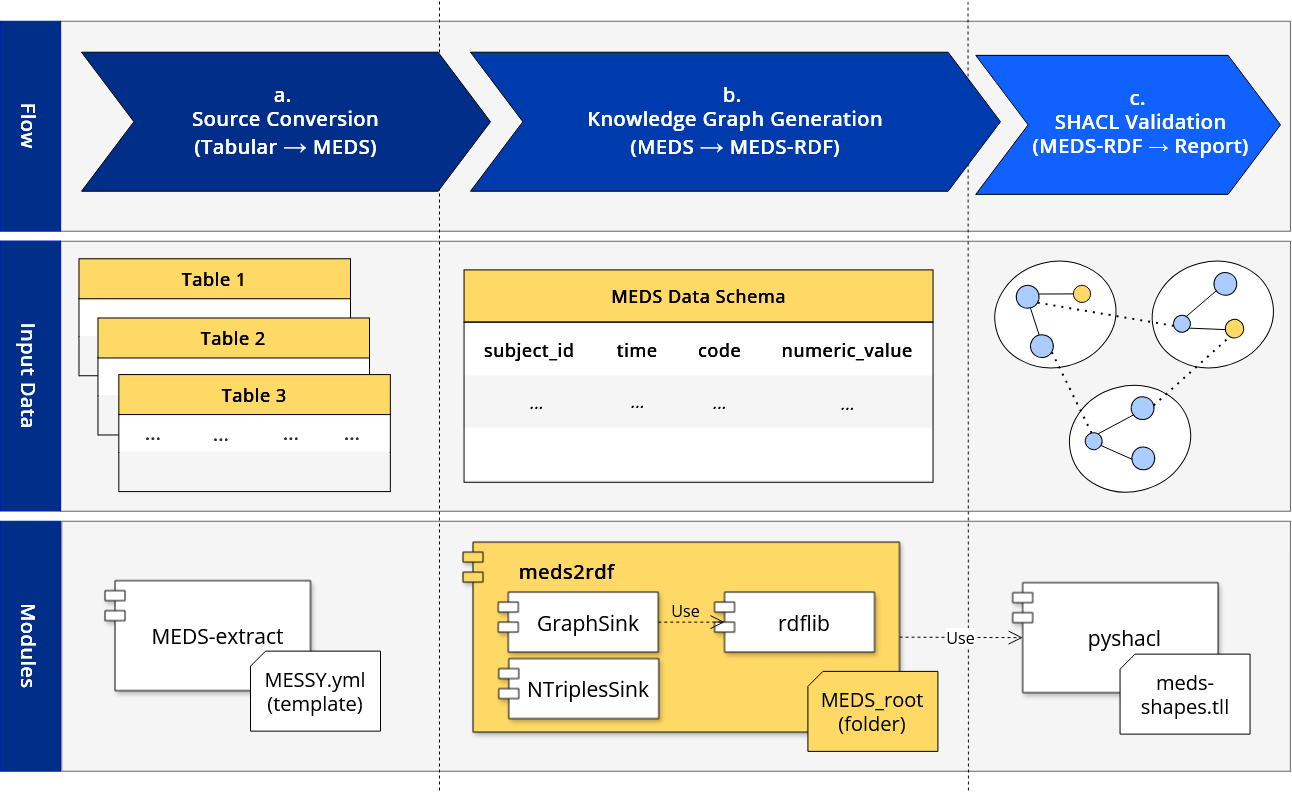
\includegraphics[width=\textwidth]{figures/paper3/fig0.png}
  \caption{Overview of the end-to-end MEDS-RDF transformation pipeline, illustrating (a) normalization and extraction of tabular data into MEDS event tuples, optional if data are already in MEDS, (b) transformation into MEDS-RDF KGs compliant with the MEDS-OWL ontology, and (c) optional SHACL-based validation and serialization into standard RDF formats.}
  \label{fig:paper3_meds-to-rdf-etl}
\end{figure*}
%
%
\paragraph{Evaluation Datasets.}\label{sec:paper3_datasets}
% \begin{table}[h]
% \caption{Datasets, with MEDS ETL support, used for evaluation. %All real-world datasets require credentialed access via PhysioNet. MEDS ETL links point to publicly available conversion pipelines
% }\label{tab:datasets}
% \begin{tabular*}{\tblwidth}{@{}L@{}R@{}C@{}C@{}C@{}}
% \toprule
% \textbf{Dataset} & \textbf{$\sim$ Stays} & \textbf{Version} &
% \textbf{Origin} & \textbf{Published}
% \\ % Table header row
% \midrule
% NEUROVASC & 10,000  & v1.0  & France & 2025  %& Synthetic care-pathway cohort for ruptured intracranial aneurysm patients
% \\
% NWICU     & 25,000  & v0.1.0 
% & USA    & 2023  %& Single-centre ICU database from Northwestern Memorial Hospital 
% \\
% MIMIC-IV  & 73,000  & v3.1   
% & USA    & 2020  %& Single-centre ICU database from Beth Israel Deaconess Medical Center 
% \\
% eICU      & 201,000 & v2.0  & USA    & 2017  %& Multi-centre ICU database spanning 208 US hospitals 
% \\

% \bottomrule
% \end{tabular*}
% \end{table}
We evaluated the MEDS-OWL framework on four datasets. NEUROVASC \cite{jhee_predicting_2025} is a synthetic open cohort describing care pathways of 10,000 patients hospitalised for ruptured intracranial aneurysms, generated from real-world EHR data at Nantes University Hospital, France. eICU \cite{pollard_eicu_2018} is a large multi-centre ICU database comprising approximately 201,000 admissions. MIMIC-IV \cite{johnson_mimic-iv_2023} contains de-identified EHR data for about 73,000 ICU stays and is one of the most widely used benchmarks in clinical informatics. NWICU \cite{moukheiber_northwestern_2024} is a single-centre ICU database covering approximately 25,000 stays. Access to eICU, MIMIC-IV, and NWICU requires credentialed PhysioNet registration and completion of a data-use agreement.

\paragraph{Round-Trip Fidelity Evaluation.}\label{sec:paper3_fidelity}
To assess whether the MEDS-RDF transformation preserves information faithfully, beyond the structural statistics reported in Section~\ref{sec:paper3_usage-examples}, we conducted a \emph{round-trip fidelity} evaluation across all four datasets. For each dataset, we (\textit{i}) converted five independent subsamples, each comprising MEDS events from 100 randomly selected patients, to RDF using \texttt{meds2rdf}, (\textit{ii}) reconstructed a tabular representation from the resulting RDF graph, and (\textit{iii}) compared the reconstructed data with the original MEDS source in terms of structural completeness and field-level fidelity. Detailed sampling procedures, metric definitions, and matching criteria are provided in the Suppl. Section \ref{sec:paper3_supp-fidelity}. The resulting fidelity measures are reported in Section~\ref{sec:paper3_evaluate-meds-rdf-conversion}.

\subsubsection{Graph Representation of Clinical Events}\label{sec:paper3_enrichment}
MEDS-RDF represents clinical events using \texttt{meds:hasSubject}, \texttt{meds:hasCode}, \texttt{meds:codeString}, and \texttt{meds:*Value} (Suppl. Table~\ref{tab:paper3_events}). In the base representation, all subject--event links use the generic \texttt{meds:hasSubject} predicate. To investigate how semantic granularity affects graph representation, \texttt{meds2rdf} provides a lightweight enrichment mechanism that specializes only the generated RDF instances, leaving the MEDS-OWL ontology unchanged. It derives more specific subject--event predicates from the event code string, which uses the \texttt{//} separator to encode progressively finer event information, as in \texttt{ATC//C08CA06} or \texttt{ICD//10//OBH17EZ}. This yields three representation variants (Figure~\ref{fig:paper3_meds-rdf-variants}): \emph{MEDS-RDF-Base}, which retains the generic \texttt{meds:hasSubject} relation; \emph{MEDS-RDF-Partial}, which specializes the relation using the event type before the first \texttt{//}; and \emph{MEDS-RDF-Full}, which further incorporates the complete code string, including the value-bearing segment.

For the enriched variants, predicates are generated deterministically by splitting the code string on non-alphanumeric delimiters, converting the resulting tokens to camelCase, and prefixing them with \texttt{has}. Codes without \texttt{//} produce identical Partial and Full predicates, while for codes containing multiple \texttt{//} separators, only the first separates the event type from the remaining code; subsequent separators are replaced with underscores to form valid normalized URIs.

% \subsection{Graph Representation of Clinical Events}\label{sec:enrichment}
% In MEDS-RDF, clinical events are represented using the predicates \texttt{meds:hasSubject}, \texttt{meds:hasCode}, \texttt{meds:codeString}, and \texttt{meds:*Value} (see Suppl. Table~\ref{tab:events}). While event attributes are explicitly modeled, the relation connecting a subject to an event is, in the base formulation, a single undifferentiated predicate (\texttt{meds:hasSubject}) that is shared across all event types.
% To investigate the effect of semantic granularity in graph construction, we introduce a lightweight semantic enrichment mechanism in \texttt{meds2rdf}. This mechanism refactors only the generated RDF instances, leaving the MEDS-OWL ontology unchanged, and replaces the generic subject--event relation with more specific predicates derived from the string associated with event codes. Such codes are of the form "event\_type//event\_subtype" where the separator // separates various levels of details of the event such as in "ATC//C08CA06" or "ICD//10//OBH17EZ". Our use of this specialisation of predicates yields three graph representation variants with increasing levels of semantic specificity, as illustrated in Figure~\ref{fig:meds-rdf-variants}:
% \begin{itemize}
%   \item \textbf{MEDS-RDF-Base}: the standard representation aligned with MEDS-OWL, where all subject--event links are expressed via \texttt{meds:hasSubject}.
%   \item \textbf{MEDS-RDF-Partial}: the subject--event relation is specialized using the event type, obtained from the code string segment preceding the first occurrence of the \texttt{//} separator.
%   \item \textbf{MEDS-RDF-Full}: the relation is further specialized using the complete code string, including the value-bearing segment following the last \texttt{//}, producing predicates that encode both event type and value.
% \end{itemize}

% For both enriched variants, predicates are automatically generated by \texttt{meds2rdf} through a deterministic transformation that splits code strings on non-alphanumeric delimiters, converts the resulting tokens to camelCase, and prefixes them with \texttt{has}. In the absence of a value segment (i.e., codes without the \texttt{//} delimiter), the partial and full variants coincide. In the case of more than one \texttt{//} delimiter, only the first is treated as the separator between the code and value segments; all subsequent occurrences are replaced with underscores (\texttt{\_}) to produce a valid, normalized URI.
% %Figure~\ref{fig:meds-rdf-variants} illustrates the three representations for the same example event, highlighting how progressively richer predicate semantics modify the structure of the resulting graph.
 
\begin{figure*}[h]
  \centering
  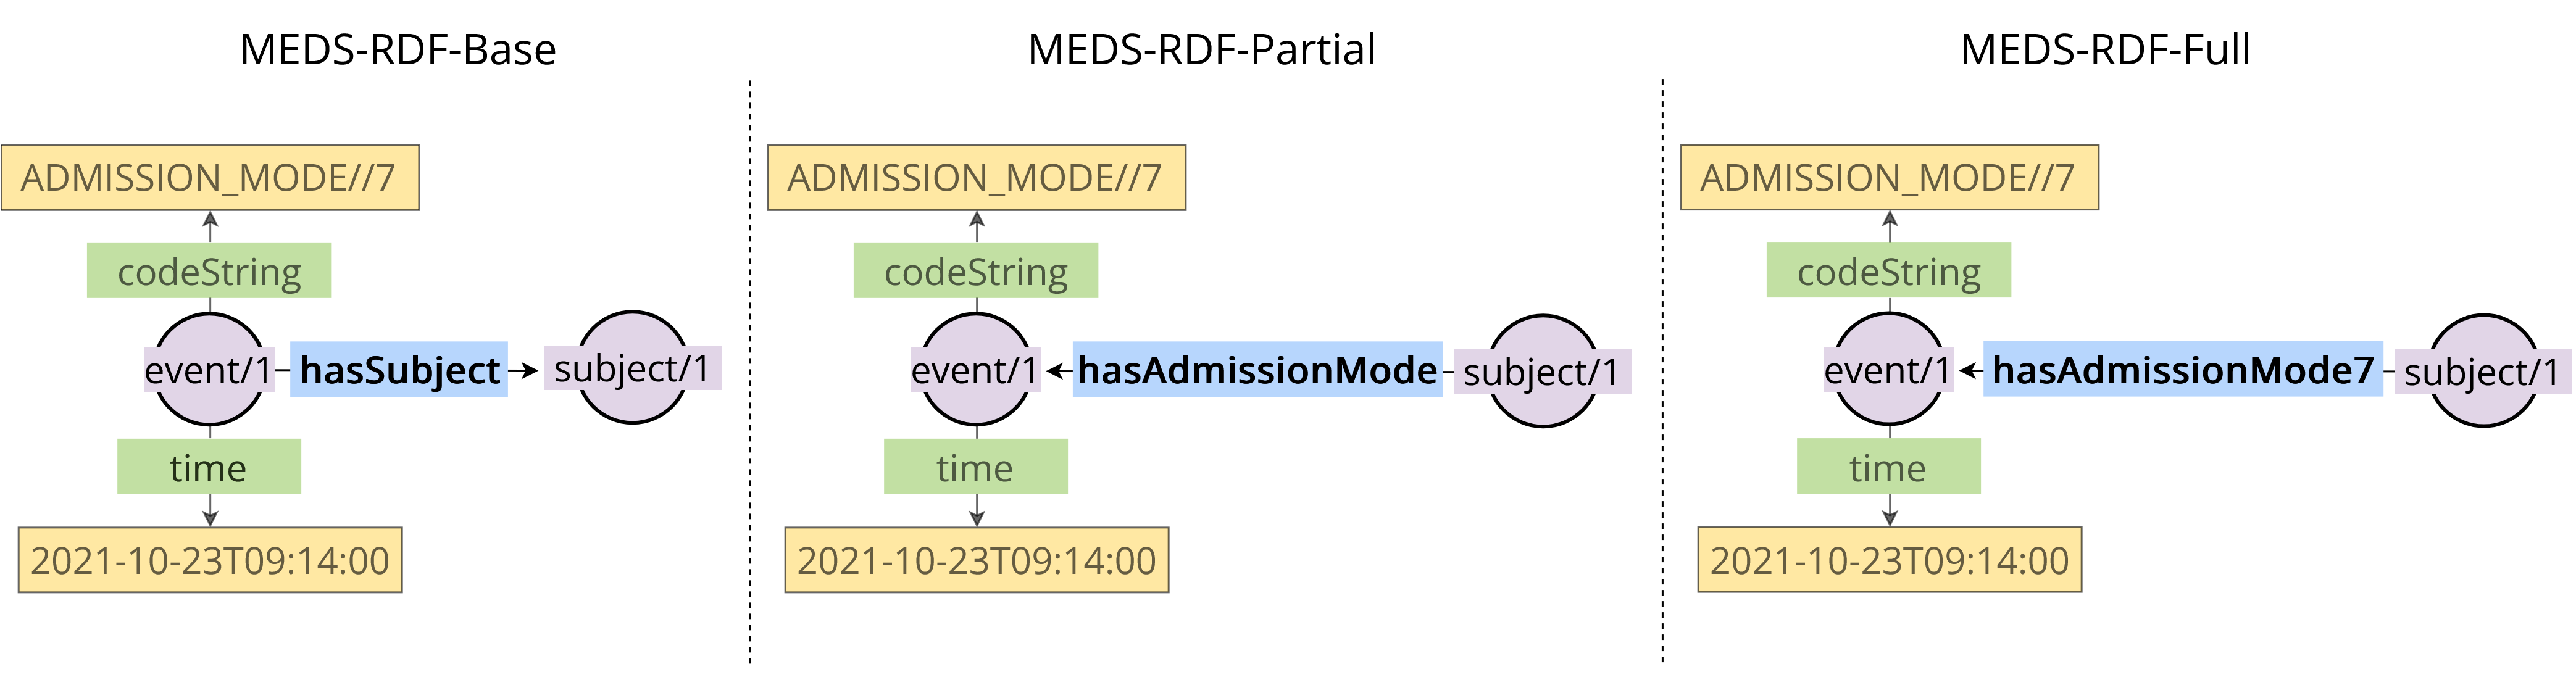
\includegraphics[width=\textwidth]{figures/paper3/fig5.png}
  \caption{MEDS-RDF representation variants of the same event (\texttt{Admission\_Mode//7}) under the three subject--event linking strategies.}
  \label{fig:paper3_meds-rdf-variants}
\end{figure*}
 
\subsubsection{Patient Outcome Prediction}\label{sec:paper3_prediction-task}
\paragraph{Prediction Tasks.}
To evaluate whether MEDS-RDF schema granularity affects downstream clinical prediction, and whether such effects generalize, we construct a multi-task predictive benchmark over MIMIC-IV using the 11 prediction tasks in Table~\ref{tab:paper3_mimic-tasks}. These latter are common prediction tasks, and we reproduce them by leveraging the ACES (Automatic Cohort Extraction System) definitions published by \cite{mcdermott_mimic-iv_2025} (see Section~\ref{sec:paper3_exp-pipeline}, Stage 2, for details). Each task is cast as a node classification problem over the corresponding MEDS-RDF graph, with patient nodes labelled according to the task-specific binary outcome. 
%
\begin{table*}[h]
\centering
\caption{A collection of various common predictive tasks on MIMIC-IV~\cite{mcdermott_mimic-iv_2025}}
\label{tab:paper3_mimic-tasks}
\begin{tabular}{p{4.8cm} p{8.4cm}}
\hline
\textbf{Task Name} & \textbf{Description} \\
\hline
First 24h in-hospital mortality & Predict mortality within a hospital admission using the first 24 hours of data from that admission. \\
First 48h in-hospital mortality & Predict mortality within a hospital admission using the first 48 hours of data from that admission. \\
First 24h in-ICU mortality & Predict mortality within an ICU admission using the first 24 hours of data from that admission. \\
First 48h in-ICU mortality & Predict mortality within an ICU admission using the first 48 hours of data from that admission. \\
Hospital LOS $>$3 days & Predict a hospital length of stay greater than 3 days, using the first 48 hours of data after admission.%, with a 24-hour gap between the input and target windows; patients who die or are discharged during the gap window are excluded. \\
\\
ICU LOS $>$3 days & Predict an ICU length of stay greater than 3 days, using the first 48 hours of data after ICU admission.%, with a 24-hour gap between the input and target windows; patients who die or are discharged during the gap window are excluded. \\
\\
30d post-hospital-discharge mortality & Predict mortality within 30 days after discharge. \\
1y post-hospital-discharge mortality & Predict mortality within 1 year after discharge. \\
30d re-admission & Predict hospital readmission within 30 days of discharge. \\
Myocardial infarction 1--5Y phenotyping & Predict myocardial infarction (MI) incidence 1--5 years after an hospital admission. \\
CKD onset in diabetics 5Y from kidney panel & Predict chronic kidney disease (CKD) onset in diabetic patients within 5 years of any kidney panel laboratory test. \\
\hline
\end{tabular}
\end{table*}
 %
 %
 
\paragraph{Architecture.}

We use a Relational Graph Convolutional Network (RGCN)~\cite{schlichtkrull_2018} as a common downstream model for all experiments, because it has been shown to provide competitive performance for entity classification against alternative graph-based approaches~\cite{schlichtkrull_2018}. We keep the architecture, hyperparameters, and training protocol fixed across graph variants, so that schema granularity (MEDS-RDF-Base, -Partial, and -Full) is the only experimental variable. RGCN is well suited to this comparison because it uses relation-specific transformations for different relation types and directions~\cite{schlichtkrull_2018}, making the learned representations sensitive to differences in predicate specialization.

For a graph $G = (\mathcal{V}, \mathcal{E}, \mathcal{R}, \mathcal{X})$ with node set $\mathcal{V}$, edge set $\mathcal{E}$, relation set $\mathcal{R}$, and initial embeddings $\mathcal{X} \in \mathbb{R}^{n \times d_0}$, the first-layer representation of target (patient) node $i$ is
\[
h_i^{(1)} =
\sigma
\left(
\sum_{r \in \mathcal{R}}
\sum_{j \in \mathcal{N}_i^r}
\frac{1}{c_{i,r}}
W_r^{(0)} x_j
+
W_0^{(0)} x_i
\right),
\]
where $\mathcal{N}_i^r$ is the neighborhood of $i$ under relation $r$, $c_{i,r}$ a normalization constant, $W_r^{(0)}$ the relation-specific weights, $W_0^{(0)}$ the self-connection weight, and $\sigma$ a nonlinear activation. We apply basis-decomposition regularization~\cite{schlichtkrull_2018} ($B=8$) to control parameter growth, which is especially important for MEDS-RDF-Full given its larger relation set. 

Since MEDS-RDF encodes attributes such as age and lab values as RDF literals, we adopt the RGCN+Literals extension~\cite{kristiadi_incorporating_2019}: literals are mapped to dense vectors via an MLP, $x_{\mathrm{literal}} = \sigma(Wv+b)$, and inserted into $\mathcal{X}$ before message passing.

After $L$ RGCN layers, each patient node $p \in \mathcal{P}$ is projected to a scalar logit $h_p$, trained with binary cross-entropy against the clinical outcome. Suppl. Figure~\ref{fig:paper3_rcgn+lit} shows the overall architecture.

\paragraph{Implementation.} We implement a two-layer RGCN with literal-aware input encoding using PyTorch Geometric's \texttt{RGCNConv}. Each node receives a type-specific base learnable embedding, with literal-bearing nodes additionally encoding their scalar value through $\mathrm{Linear}(1,d_{\text{embed}})$ and PReLU, masked by literal presence. The two \texttt{RGCNConv} layers use basis-decomposed relation weights, with dimensions $d_{\text{embed}}\rightarrow d_{\text{hidden}}\rightarrow1$ and PReLU activation between layers. Because all tasks are binary, the final layer outputs one patient-level logit, optimized with \texttt{BCEWithLogitsLoss}; at inference, the sigmoid probability is thresholded at 0.5 for hard predictions, while both class probabilities are used to compute AUC and AUPRC. Models were trained independently for the 11 tasks with $d_{\text{embed}}=d_{\text{hidden}}=32$, no dropout, Adam optimization ($\mathrm{lr}=5\times10^{-4}$, weight decay $=5\times10^{-4}$), and up to 2,000 epochs with early stopping (patience 50, minimum validation-loss improvement $10^{-4}$), restoring the best validation checkpoint. We used two layers because the compact MEDS-RDF topology allows information to propagate from subject nodes through events to their attributes within two message-passing steps. Sensitivity analyses with three, four, and five layers showed no predictive improvement while increasing computational cost (Suppl. Table~\ref{tab:paper3_rgcn-depth}).

% \paragraph{Implementation.}
% We implement a 2-layer RGCN with literal-aware input encoding using PyTorch Geometric's \texttt{RGCNConv}. Each node $i$ receives an initial feature vector based on its type: literal-bearing nodes (e.g., the \texttt{textValue}/ \texttt{numericValue} of a MEDS event) have their raw scalar value projected through $\mathrm{Linear}(1, d_{\text{embed}})$ followed by a PReLU activation, masked by an indicator of literal presence, and added to a base learnable embedding shared across all nodes. These features pass through two \texttt{RGCNConv} layers $(d_{\text{embed}} \rightarrow d_{\text{hidden}})$ then $(d_{\text{hidden}} \rightarrow 1)$ each using basis-decomposed relation weights, with a PReLU activation and dropout between layers. As every task is binary, the second layer outputs a single logit per patient node rather than a $K$-way softmax, trained by minimizing binary cross-entropy with logits (\texttt{BCEWithLogitsLoss}). At inference, the logit is passed through a sigmoid to obtain $P(y_p = \text{True})$, thresholded at 0.5 for hard predictions; the complementary probability $1 - P(y_p = \text{True})$ is used alongside to compute AUC and AUPRC. Models are trained independently for each of the 11 tasks, with $d_{\text{embed}} = d_{\text{hidden}} = 32$, dropout $=0$, and Adam optimization ($\text{lr}=5\times10^{-4}$, weight decay $=5\times10^{-4}$) for up to 2,000 epochs with early stopping (patience 50 epochs on validation loss, minimum improvement delta $10^{-4}$), restoring the best validation checkpoint at the end of training.

% We use two RGCN layers because thanks to the compact topology of MEDS-RDF, two message-passing steps are sufficient to propagate information from patient/subject nodes through event nodes to their leaf-level attributes. To assess the sensitivity of this choice, we additionally evaluated RGCN+lit models with three, four, and five layers under the same experimental protocol. These deeper configurations did not improve predictive performance while increasing computational cost (Suppl. Table~\ref{tab:rgcn-depth}).

\paragraph{Tabular learning baselines.}
%\textcolor{blue}{ac: \textbf{Tab learning as a baseline}. I think we should have few works about you tab learning baseline here (before Stage 5 of 2.4.  }
Tabular methods, particularly gradient-boosted tree ensembles such as XGBoost~\cite{Chen_2016}, are well established as highly competitive with neural network approaches on structured and longitudinal medical data~\cite{oufattole_meds-tab_2024}. We therefore contextualize RGCN+Literals against three tabular baselines spanning a range of model complexity: Logistic Regression, Random Forest, and XGBoost. Because these baselines receive no graph or relational structure, comparing them against RGCN+Literals isolates the predictive contribution of the relational representation itself, independent of schema granularity. Their construction and evaluation are detailed in Stages~5 and~6 of Section~\ref{sec:paper3_exp-pipeline}.

\paragraph{SHAP-guided relation pruning.}
%\textcolor{blue}{ac: \textbf{SHAP-guided pruning}. I think we should have a paragraph here describing the approach of pruning based on SHAPE values.}
MEDS-RDF-Full introduces substantially more relation types than MEDS-RDF-Base or -partial (Section~\ref{sec:paper3_enrichment}), which increases GPU memory requirements and risks diluting the RGCN's capacity across many low-information relations. To reduce this burden, we reuse the XGBoost baseline\cite{xu_aces_2025} introduced above to identify the most predictive event types: SHAP (SHapley Additive exPlanations) values are computed on the trained XGBoost model, and only the event types ranked highest by SHAP importance are retained. SHAP is a post-hoc explainability technique that uses a game-theoretic approach to assign each feature a Shapley value, quantifying its contribution to a model's output for a given prediction~\cite{nohara_explanation_2021}. This retained event set is then used to prune the patient timeline before MEDS-RDF conversion. This procedure is applied identically across schema variants, so that pruning isolates schema granularity as the sole experimental variable. The specific instantiation of this procedure for MIMIC-IV is given in Stage~4 of Section~\ref{sec:paper3_exp-pipeline}.

\subsubsection{Experimental Pipeline for MIMIC-IV}\label{sec:paper3_exp-pipeline}
The following section summarises the end-to-end experimental pipeline, which proceeds through six sequential stages.
 
\paragraph{Stage 1 -- MEDS conversion.} Unlike NEUROVASC, which requires a custom MEDS-extract mapping configuration (Section~\ref{sec:paper3_usage-examples}), MIMIC-IV is already distributed in MEDS format via its publicly available MEDS-ETL pipeline~\cite{mcdermott_mimic-iv_2025,van_de_water_mimic-iv_2025}, so no custom mapping configuration is required upstream. The downloaded MIMIC-IV-MEDS dataset serves as the single source for all subsequent stages.
 
\paragraph{Stage 2 -- Cohort extraction.} The 11 prediction task cohorts (Table~\ref{tab:paper3_mimic-tasks}) are extracted from MIMIC-IV-MEDS using ACES~\cite{xu_aces_2025}, a reproducible, configuration-driven framework that identifies patient windows satisfying each task's inclusion criteria (e.g., index time, label window, exclusion conditions) directly from the MEDS event stream without requiring task-specific data transformations.
 
\paragraph{Stage 3 -- Balanced subsampling and preprocessing.} For each task, 5 independent subsamples of 1,000 patients are drawn, each composed of a set of 500 patients with a false  class label and another of 500 with a true label, %, stratified by outcome class 
to ensure balanced training conditions. The sole exception is \emph{CKD onset in diabetics 5Y from kidney panel}, where the pool of positive patients is insufficient for five independent draws of 500 each as the dataset only contains 443 positives. For this task, subsamples are capped at 886 patients in total, same positive, but distinct negative patients were drawn in each subsamples of this task. Within each subsample, timestamped events are aggregated by a task-specific time window (matching the input window defined in Table~\ref{tab:paper3_mimic-tasks}: 24h, 48h, or full history to prediction time): numerical measurements are represented as minimum and maximum over the window, static codes are kept as-is. %, and dynamic codes are counted.
 
\paragraph{Stage 4 -- SHAP-guided relation pruning.}
We instantiate the pruning procedure introduced in Section~\ref{sec:paper3_prediction-task} as follows. For each task, the XGBoost baseline (Section~\ref{sec:paper3_prediction-task}) is trained on a tabular representation of the Stage~3 subsample, using one feature per MEDS event type. %as summarized in Table~\ref{tab:feature-mapping}. 
SHAP values are then computed on this trained model using \texttt{TreeExplainer}, with per-feature importance taken as the mean absolute SHAP value, computed separately for each output class (TRUE/FALSE); the retained feature set for threshold $\theta$ is the union of per-class features whose importance is at or above the $\theta$-th quantile of that class's distribution. At $\theta = 0.90$ (top 10\%), MEDS events whose code is not in the retained set are dropped from the preprocessed dataset before any RDF conversion, applied identically across schema variants. The choice of $\theta = 0.90$ is justified empirically in Section~\ref{sec:paper3_results-ablation}.

% \begin{table}[h]
% \caption{Mapping from MEDS event types to tabular features used for XGBoost training.}\label{tab:feature-mapping}
% \begin{tabular}{p{1.4cm} p{3.3cm} l}
% \toprule
% \textbf{Event type} & \textbf{Feature construction} & \textbf{Example} \\
% \midrule
% Static\break{}Categorical & One-hot encoding from the code suffix & \texttt{GENDER} $\rightarrow$ \texttt{F} \\
% Static\break{}Numeric & Value retained as-is (single occurrence) & \texttt{LAB//51277} \\
% Dynamic\break{}Categorical & Occurrence count within the observation window & \texttt{DIAGNOSIS//X\_count} \\
% Dynamic\break{}Numeric & Mean value across all occurrences within the window & \texttt{LAB//51277} \\
% \bottomrule
% \end{tabular}%
% \end{table}

\paragraph{Stage 5 -- Graph and tabular representation.} Each pruned MEDS subsample is then branched into two parallel representations used for the two classes of models evaluated:
\begin{itemize}
  \item \emph{MEDS-RDF (for RGCN):} the pruned MEDS dataset is converted to RDF using \texttt{meds2rdf} (Section~\ref{sec:paper3_meds2rdf}), instantiated independently in each of the three subject-event linking modes (MEDS-RDF-Base, -partial, and -full) described in Section~\ref{sec:paper3_enrichment}. Because the unpruned full-granularity graph could not be loaded into GPU memory on MIMIC-IV, MEDS-RDF-Full is evaluated only on the SHAP-pruned subset; MEDS-RDF-Base and -partial are evaluated on both the entire (unpruned) dataset and the pruned subset for reference.
  \item \emph{Tabular (for tabular baselines):} the same pruned MEDS subsample is pivoted into a wide feature matrix (one feature per $(code, value)$ pair), used to train and evaluate Logistic Regression, Random Forest, and XGBoost models.
\end{itemize}

\paragraph{Stage 6 -- Prediction and evaluation.}
Both the RGCN + Literals model (Section~\ref{sec:paper3_prediction-task}) and the tabular baselines (Section~\ref{sec:paper3_results-schema}) are trained and evaluated using a stratified 10-fold cross-validation protocol (80\% training, 10\% validation, 10\% test per fold; random seed 77), with identical patient assignments across models to ensure paired comparisons. The 10-fold cross-validation is performed independently for each of the 5 patient subsamples generated in Stage~3. All tasks are binary classification problems, and cohorts are class-balanced by construction. For each fold, we report per-class F1-scores (positive and negative), along with Macro-F1, Weighted-F1, Accuracy, AUC, and AUPRC. AUC and AUPRC are computed using the predicted probability of the positive class $P(y=\text{True})$, with the negative class implicitly defined as $1 - P(y=\text{True})$. Final results are aggregated across the 5 subsamples and their 10 cross-validation folds and are reported as the mean and standard deviation of the resulting fold-level scores. To assess whether differences in predictive performance between RGCN2+lit and XGBoost were statistically significant, we performed two-sided paired t-tests separately for each of the 11 prediction tasks. %For each task, the five subsample-level Macro-F1 scores obtained from RGCN2+lit and XGBoost were treated as paired observations, since the same patient subsamples and cross-validation assignments were used for both models. The test was performed on the unrounded Macro-F1 values, with statistical significance assessed at $p < 0.05$.

\subsection{Results}\label{sec:paper3_results}
This section evaluates MEDS-OWL and \texttt{meds2rdf} across three dimensions: preservation of the MEDS event model in RDF, scalability to large clinical datasets, and the impact of semantic expressiveness on downstream predictive performance. We first characterize the ontology mapping and end-to-end conversion process (Sections~\ref{sec:paper3_ontology-mapping} and~\ref{sec:paper3_usage-examples}), then evaluate round-trip fidelity and conversion scalability (Sections~\ref{sec:paper3_fidelity} and
\ref{sec:paper3_scalability}), and finally assess predictive performance across alternative graph representations (Section~\ref{sec:paper3_prediction-results}).

\subsubsection{Ontology Overview and Mapping Results}\label{sec:paper3_ontology-mapping}
MEDS-OWL in its first release comprehends  13 classes, 10 object properties, 20 data properties, and 24 OWL axioms, and it is accompanied by example RDF instances and a SHACL validation suite. MEDS-OWL is illustrated in Suppl. Figure~\ref{fig:paper3_ontology-diagram}. %and its documentation is available on Zenodo and GitHub~\citep{marfoglia_teamhekameds-ontology_2025}.

Mappings between MEDS core data schema elements and MEDS-OWL are reported in Suppl. Tables \ref{tab:paper3_events}-\ref{tab:paper3_labels}. Suppl. Table \ref{tab:paper3_events} reports those to the \texttt{meds:Event} class. In MEDS-OWL, events are required to be associated with exactly one subject and exactly one code, while temporal and value-related attributes are optional and for this reason constrained by cardinality restrictions. Table \ref{tab:paper3_codes} reports mappings to the \texttt{meds:Code} class. Code metadata is modeled explicitly as individuals of type \texttt{meds:Code}, which enables reusability, hierarchical organization, and linkage to external terminologies. Dataset-level provenance and conversion metadata are represented by the \texttt{meds:DatasetMetadata} class, which is aligned with both \texttt{dcat:Dataset} and \texttt{prov:Entity}. Cardinality constraints are enforced at the OWL level. The corresponding mappings are shown in Table \ref{tab:paper3_dataset}. Finally, Table \ref{tab:paper3_labels} reports the mapping for dataset splits and supervised learning labels. Dataset partitions are modeled as predefined individuals of class \texttt{meds:SubjectSplit}, while label samples are represented as instances of \texttt{meds:SubjectLabel} with exactly one label value.

%The \textbf{meds2rdf library} that implements the mapping rules is available on Zenodo and GitHub \citep{marfoglia_teamhekameds2rdf_2025}.

\subsubsection{MEDS-RDF Transformation Pipeline}\label{sec:paper3_usage-examples}
We illustrate the MEDS-RDF transformation using two complementary datasets: NEUROVASC, which provides a controlled synthetic cohort, and the 100-patient MIMIC-IV demo~\cite{mcdermott_mimic-iv_2025}, which illustrates application to real-world EHR data. The complete workflows, including the intermediate MEDS representation and provenance links, are shown in Suppl. Figures~\ref{fig:paper3_etl-conversion} and~\ref{fig:paper3_provenance-instance}. \texttt{meds2rdf} transformed the 245,015 NEUROVASC events from 10,000 subjects into 1.33 million RDF triples, while the MIMIC-IV demo produced 916,166 events and 6.41 million triples from 100 subjects. In both cases, the resulting graphs instantiate the corresponding MEDS-OWL classes and preserve dataset, split, and provenance metadata. Detailed graph statistics and ontology instantiation counts are provided in Suppl. Section~\ref{sec:paper3_supp-transformation-examples}. The MIMIC-IV example uses the fixed 100-patient demo solely for illustration; the systematic round-trip fidelity and scalability analyses instead use the full MIMIC-IV dataset together with NEUROVASC, eICU, and NWICU.

\subsubsection{Correctness and Scalability of MEDS-RDF Transformation}\label{sec:paper3_evaluate-meds-rdf-conversion}
We evaluate the MEDS-RDF transformation along two complementary dimensions: \emph{round-trip fidelity}, which assesses whether MEDS information can be reconstructed from RDF, and \emph{scalability and performance}, which measures the computational cost of generating RDF graphs from complete clinical datasets.

\paragraph{Round-Trip Fidelity Evaluation.}
Table~\ref{tab:paper3_fidelity} summarises the round-trip fidelity results across the four datasets using the protocol described in Section~\ref{sec:paper3_fidelity}. For each dataset, $K=5$ independent samples of $N=100$ patients were evaluated. Structural and subject completeness, as well as \texttt{subject\_id}, \texttt{code}, \texttt{time}, and \texttt{numeric\_value} fidelity, are 1.0 across all datasets, with zero numeric error and temporal deviation. The MIMIC-IV results reported here are based on random samples from the complete dataset and therefore differ from the fixed 100-patient \emph{MIMIC-IV demo} subset used in Section~\ref{sec:paper3_usage-examples}; complete-dataset conversion is instead assessed in Section~\ref{sec:paper3_scalability}.

The only deviations from perfect fidelity occur in \texttt{text\_value} and code completeness for some real-world datasets. Text-value fidelity is 0.981 for MIMIC-IV and 0.9998 for both eICU and NWICU, reflecting normalization of special or control characters during RDF conversion. Code completeness is 0.9998 for MIMIC-IV and 0.9996 for eICU, due to a small number of non-conformant source codes that are dropped during conversion. These deviations are limited to free-form or loosely validated source content; the core schema-defined MEDS fields are preserved exactly.

Duplicate-key events, defined by identical (\texttt{subject\_id}, \texttt{time}, \texttt{code}) values, occur in all real-world datasets and are excluded from join-based fidelity metrics because they cannot be uniquely matched during reconstruction. They account for 7.8--11.0\% of MIMIC-IV events, 0.2--0.5\% of eICU events, and 1.8--2.3\% of NWICU events; approximate matching yielded \texttt{numeric\_value} fidelity of 1.0 for these events.

\begin{table*}[h]
\centering
\caption{Round-trip fidelity results across four MEDS datasets (sampled at 100 patients, averaged over 5 samples). Subject identifier, code, time, and numeric value fidelity are 1.0 across all datasets; text value fidelity is slightly below 1.0 for the real-world datasets due to RDF-compatible normalisation of special characters in free-text fields. Structural losses are ontology-level limitations present in all cases.}
\label{tab:paper3_fidelity}
\resizebox{\textwidth}{!}{%
\begin{tabular}{lrrrr}
\hline
\textbf{Metric} & \textbf{NEUROVASC} & \textbf{MIMIC-IV} & \textbf{eICU} & \textbf{NWICU} \\ \hline
Events (original / reconstructed) & 251 / 251 & 161,356 / 161,356 & 1,373,226 / 1,373,226 & 157,884 / 157,884 \\
Structural completeness & 1.0 & 1.0 & 1.0 & 1.0 \\
Subjects (original / reconstructed) & 100 / 100 & 100 / 100 & 100 / 100 & 100 / 100 \\
Subject completeness & 1.0 & 1.0 & 1.0 & 1.0 \\ \hline
Fidelity — \texttt{subject\_id} & 1.0 & 1.0 & 1.0 & 1.0 \\
Fidelity — \texttt{code} & 1.0 & 1.0 & 1.0 & 1.0 \\
Fidelity — \texttt{time} & 1.0 & 1.0 & 1.0 & 1.0 \\
Fidelity — \texttt{numeric\_value} & 1.0 & 1.0 & 1.0 & 1.0 \\
Fidelity — \texttt{text\_value} & 1.0 & 0.981 & 0.9998 & 0.9998 \\
Numeric max abs.\ error & 0.0 & 0.0 & 0.0 & 0.0 \\
Numeric mean abs.\ error & 0.0 & 0.0 & 0.0 & 0.0 \\
Temporal max $\Delta$ (s) & 0.0 & 0.0 & 0.0 & 0.0 \\
Temporal mean $\Delta$ (s) & 0.0 & 0.0 & 0.0 & 0.0 \\
\hline
Codes (original / reconstructed) & 91 / 91 & 5,608 / 5,607 & 2,225 / 2,224 & 3,413 / 3,413 \\
Code completeness & 1.0 & 0.9998 & 0.9996 & 1.0 \\ \hline
Null rate \texttt{numeric\_value} (orig.) & 1.000 & 0.508 $\pm$ 0.016 & 0.711 $\pm$ 0.025 & 0.405 $\pm$ 0.010 \\
Null rate \texttt{text\_value} (orig.) & 1.000 & 0.613 $\pm$ 0.076 & 0.998 $\pm$ 0.0004 & 0.995 $\pm$ 0.0007 \\
Duplicate-key rows (\% of events) & 0.0\% & 7.8–11.0\% & 0.2–0.5\% & 1.8–2.3\% \\ \hline
\end{tabular}%
}
\end{table*}

\paragraph{Scalability and Performance Evaluation.}\label{sec:paper3_scalability}
We next assess whether \texttt{meds2rdf} can perform complete conversions at scale. Conversion time and output size were measured for all four datasets, while the first and second releases of \texttt{meds2rdf} were compared on NEUROVASC, the only dataset for which the in-memory v1 conversion could be completed. Experiments were performed on Ubuntu 24.04.2 LTS using 16 AMD EPYC-Genoa cores and 32~GB of RAM.

On the complete NEUROVASC dataset, comprising 245,015 MEDS events from 10,000 patients, v1 required 39.9~s, whereas v2 completed the conversion in 15~s, corresponding to a 2.7$\times$ speedup. The v1 converter could not complete the three real-world datasets because its in-memory \texttt{rdflib.Graph} exhausted available RAM, whereas v2 successfully processed all four datasets using the streaming \texttt{NTriplesSink} strategy. Table~\ref{tab:paper3_scalability} reports conversion times and output sizes with and without gzip compression. These complete-dataset conversions are complementary to the sampled round-trip evaluation: the former measures scalability, whereas the latter evaluates information preservation.

% Please add the following required packages to your document preamble:
% \usepackage{graphicx}
\begin{table*}[h]
\centering
\caption{Scalability results for \texttt{meds2rdf} v2 (NTriplesSink) on complete conversions of all four datasets.} %The v1 converter is shown only for NEUROVASC; all real-world datasets exceeded available RAM and could not be completed.}
\label{tab:paper3_scalability}
\resizebox{\textwidth}{!}{%
\begin{tabular}{lrrrrrr}
\hline
\textbf{Dataset} & \textbf{Time (plain)} & \textbf{Size (plain)} & \textbf{Time (gzip)} & \textbf{Size (gzip)} & \multicolumn{1}{c}{\textbf{\begin{tabular}[c]{@{}c@{}}Time\\ overhead\end{tabular}}} & \multicolumn{1}{c}{\textbf{\begin{tabular}[c]{@{}c@{}}Size\\ reduction\end{tabular}}} \\ \hline
NEUROVASC & 15 s & 247 MB & 22 s & 6.9 MB & +32\% & -97\% \\
NWICU & 1h 07m 42s & 62 GB & 1h 32m 40s & 2.0 GB & +27\% & -97\% \\
eICU & 38m 31s & 41 GB & 53m 08s & 800 MB & +28\% & -98\% \\
MIMIC-IV & 17h 17m 53s & 937 GB & 25h 02m 34s & 32 GB & +31\% & -97\% \\ \hline
\end{tabular}%
}
\end{table*}
%
%
%
%
\subsubsection{Outcome Prediction Results on MIMIC-IV}\label{sec:paper3_prediction-results}
The experiments in this section assess whether increasing the semantic expressiveness of MEDS-RDF improves graph-based outcome prediction across the 11 MIMIC-IV tasks introduced in Section~\ref{sec:paper3_prediction-task}. As described in Section~\ref{sec:paper3_enrichment}, MEDS-RDF-Full assigns a distinct relation to each $(\text{code},\text{value})$ pair and exceeds available GPU memory when constructed from the complete MIMIC-IV dataset. We therefore apply SHAP-guided event pruning before RDF conversion, using the same filtered event set for all three schema variants. %This ensures that performance differences between MEDS-RDF-Base, MEDS-RDF-Partial, and MEDS-RDF-Full reflect semantic representation rather than differences in the underlying clinical information.

The results are presented in four stages. (\textit{i}) We first justify the SHAP-guided pruning strategy using a representative prediction task, examining feature importance, pruning thresholds, and the contribution of temporal and literal information. (\textit{ii}) We then evaluate the three MEDS-RDF schema variants across all 11 prediction tasks. (\textit{iii}) Next, we analyze the computational and environmental costs associated with increasing semantic granularity. (\textit{iv}) Finally, we compare the best-performing graph representation with established tabular learning baselines.

\paragraph{SHAP-guided pruning and configuration ablation.}\label{sec:paper3_results-ablation}
We first calibrated the SHAP-based retention threshold on the \emph{First 24h in-hospital mortality} task using an XGBoost model and
then fixed it for all subsequent experiments. The SHAP rankings identified a stable set of influential clinical features, led by patient age and followed by laboratory, medication, and admission-related events (Figure~\ref{fig:paper3_shap-summary}), supporting the use of a common threshold.
%
\begin{figure*}[h]
  \centering
  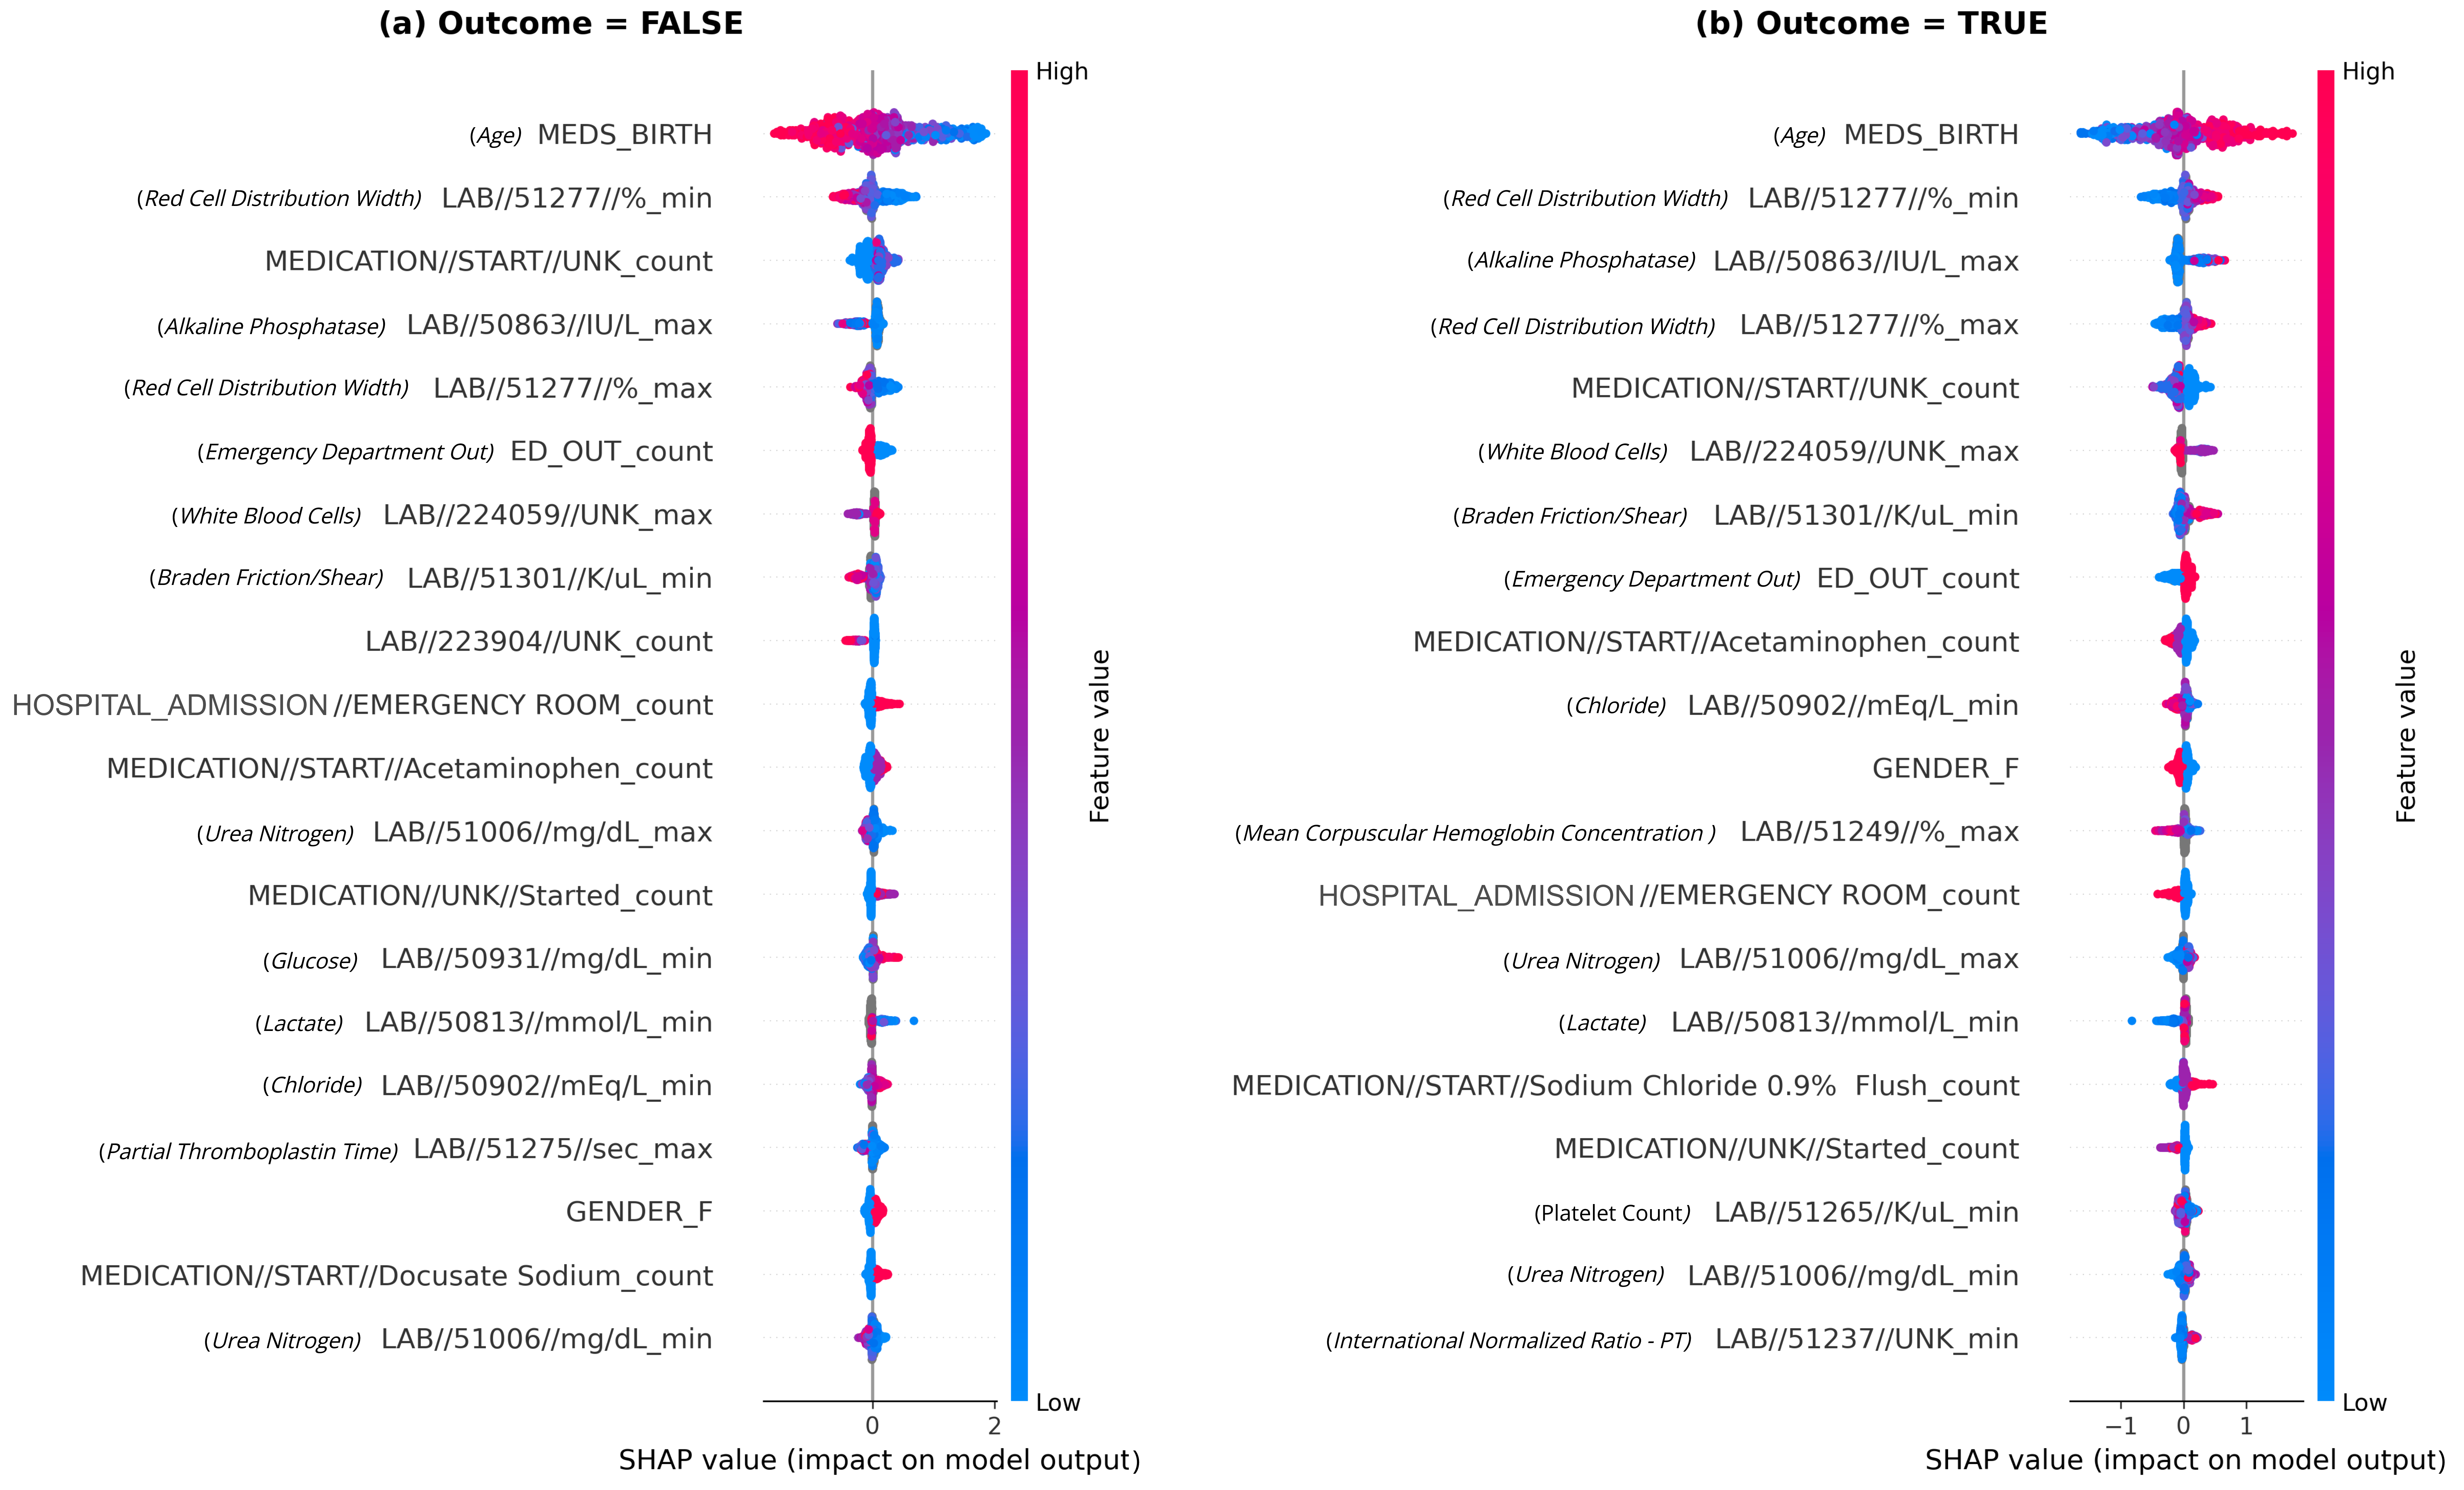
\includegraphics[width=\textwidth]{figures/paper3/fig6.png}
\caption{SHAP summary plots for the XGBoost model used to rank MEDS (code, value) features by importance for SHAP-guided relation pruning on \emph{First 24h in-hospital mortality}, reported separately for each outcome class: (a) FALSE, (b) TRUE. Each point is one patient; horizontal position is the SHAP value (contribution to model output) and colour encodes the feature's value (low to high). For readability, only the top-20 features are shown.}
  \label{fig:paper3_shap-summary}
\end{figure*}

Across MEDS-RDF-Full, varying the retention threshold from the top 1\% to 30\% yielded similar predictive performance (Macro-F1: 0.70--0.72; AUC: 0.77--0.80) while reducing the number of retained relations from 205 to 14; we therefore selected the top 10\% as a balance between graph compactness and predictive performance. At this threshold, MEDS-RDF-Full achieved a Macro-F1 of 0.72 and AUC of 0.80, compared with 0.63 and 0.69 for MEDS-RDF-Partial and 0.56 and 0.59 for MEDS-RDF-Base, respectively. Removing temporal information reduced Macro-F1 to 0.71 and AUC to 0.76, while additionally removing literal information reduced them to 0.70 and 0.75, indicating complementary contributions from temporal and literal information (Table~\ref{tab:paper3_results-ablation}).

\begin{table*}[h]
\caption{Configuration ablation on \emph{First 24h in-hospital mortality}: SHAP-pruning threshold (retained top-percentile of relations by importance), literal/temporal information, and resulting graph size. Experiments use RGCN2+lit with all-MiniLM-L6-v2 for textual values, except \emph{Full (no-time; no-txt)}, where no sentence transformer is used.}
\label{tab:paper3_results-ablation}
\resizebox{\textwidth}{!}{%
\begin{tabular}{llccccccccc}
\hline
\multicolumn{1}{c}{\multirow{2}{*}{Dataset}} & \multicolumn{1}{c}{\multirow{2}{*}{\begin{tabular}[c]{@{}c@{}}MEDS-RDF variant\end{tabular}}} & \multicolumn{1}{l}{\multirow{2}{*}{Predicates}} & \multicolumn{1}{l}{\multirow{2}{*}{Triples}} & \multicolumn{4}{c}{F1-score} & \multirow{2}{*}{Accuracy} & \multirow{2}{*}{AUC} & \multirow{2}{*}{AUPRC} \\ \cline{5-8}
\multicolumn{1}{c}{} & \multicolumn{1}{c}{} & \multicolumn{1}{l}{} & \multicolumn{1}{l}{} & False & True & Macro & Weighted &  &  &  \\ \hline
\multirow{2}{*}{Entire} & Base & 9 & \multirow{2}{*}{2,768,048} & 0.61 ±   0.06 & 0.63 ± 0.12 & 0.62 ± 0.08 & 0.62 ± 0.08 & 0.61 ± 0.06 & 0.66 ± 0.07 & 0.67 ± 0.07 \\
 & Partial & 19 &  & 0.66 ± 0.05 & 0.66 ± 0.06 & 0.66 ± 0.05 & 0.66 ± 0.05 & 0.65 ± 0.04 & 0.73 ± 0.05 & 0.72 ± 0.06 \\
\hline
  Only top 30\% & \multirow{2}{*}{Full} & 205 & \multicolumn{1}{r}{968,738} & 0.70 ± 0.04 & 0.69 ± 0.06 & 0.69 ± 0.05 & 0.69 ± 0.05 & 0.69 ± 0.05 & 0.77 ± 0.04 & 0.78 ± 0.04 \\ 
  Only top 15\% &  & 105 & \multicolumn{1}{r}{511,006} & 0.72 ± 0.05 & 0.71 ± 0.06 & 0.71 ± 0.04 & 0.71 ± 0.04 & 0.71 ± 0.04 & 0.79 ± 0.05 & 0.79 ± 0.05 \\
\hline
\multirow{5}{*}{Only top 10\%} & Base & 7 & \multirow{5}{*}{366,053} & 0.54 ± 0.15 & 0.57 ± 0.16 & 0.56 ± 0.12 & 0.56 ± 0.12 & 0.56 ± 0.06 & 0.59 ± 0.09 & 0.60 ± 0.08 \\
 & Partial & 12 &  & 0.64 ± 0.06 & 0.62 ± 0.05 & 0.63 ± 0.05 & 0.63 ± 0.05 & 0.63 ± 0.05 & 0.69 ± 0.06 & 0.67 ± 0.06 \\
 & Full & 74 &  & \textbf{0.73 ± 0.05} & \textbf{0.71 ± 0.05} & \textbf{0.72 ± 0.04} & \textbf{0.72 ± 0.04} & \textbf{0.72 ± 0.05} & \textbf{0.80 ± 0.05} & \textbf{0.79 ± 0.05} \\
 & \begin{tabular}[c]{@{}l@{}}Full (no-time)\end{tabular} & 74 &  & 0.71 ± 0.05 & 0.71 ± 0.05 & 0.71 ± 0.04 & 0.71 ± 0.04 & 0.70 ± 0.04 & 0.76 ± 0.05 & 0.75 ± 0.05 \\
 & \begin{tabular}[c]{@{}l@{}}Full (no-time;no-txt)\end{tabular} & 74 &  & 0.69 ± 0.05 & 0.70 ± 0.05 & 0.70 ± 0.04 & 0.70 ± 0.04 & 0.69 ± 0.04 & 0.75 ± 0.06 & 0.74 ± 0.06 \\
 \hline
% Only top 30\% & \multirow{4}{*}{Full} & 205 & \multicolumn{1}{r}{968,738} & 0.70 ± 0.04 & 0.69 ± 0.06 & 0.69 ± 0.05 & 0.69 ± 0.05 & 0.69 ± 0.05 & 0.77 ± 0.04 & 0.78 ± 0.04 \\ 
%Only top 15\% &  & 105 & \multicolumn{1}{r}{511,006} & 0.72 ± 0.05 & 0.71 ± 0.06 & 0.71 ± 0.04 & 0.71 ± 0.04 & 0.71 ± 0.04 & 0.79 ± 0.05 & 0.79 ± 0.05 \\
Only top 5\% & \multirow{2}{*}{Full} & 41 & \multicolumn{1}{r}{202,437} & 0.72 ± 0.06 & 0.72 ± 0.06 & 0.72 ± 0.05 & 0.72 ± 0.05 & 0.72 ± 0.06 & 0.80 ± 0.06 & 0.78 ± 0.06 \\
Only top 1\% &  & 14 & \multicolumn{1}{r}{45,892} & 0.71 ± 0.07 & 0.70 ± 0.05 & 0.70 ± 0.05 & 0.70 ± 0.05 & 0.70 ± 0.05 & 0.78 ± 0.05 & 0.76 ± 0.06 \\
\hline
\multicolumn{11}{c}{\textbf{Task : First 24h in-hospital mortality}} \\ \hline
\end{tabular}%
}
\end{table*}
 
\paragraph{Impact of semantic representation across prediction tasks.}\label{sec:paper3_results-schema}
Using the top-10\% SHAP-pruning threshold established in Section~\ref{sec:paper3_results-ablation}, we compared MEDS-RDF-Base, MEDS-RDF-Partial, and MEDS-RDF-Full across the 11 MIMIC-IV prediction tasks. Table~\ref{tab:paper3_results-illustrative} presents three representative tasks, while complete results and comparisons with Logistic Regression, Random Forest, and XGBoost are reported in Supplementary Tables~\ref{tab:paper3_results-schema-full} and~\ref{tab:paper3_results-tabular-full}. Because all pruned variants use the same filtered event set, performance differences isolate the effect of semantic specialization. Macro-F1 increased consistently with schema granularity across all 11 tasks, with MEDS-RDF-Full providing the highest Macro-F1 in every case. %On the unpruned dataset, the same progression was observed in 9 of 11 tasks; the two exceptions disappear once SHAP-guided pruning is applied. This indicate that pruning does not merely make MEDS-RDF-Full tractable, but also removes noise from rare or uninformative codes that can otherwise destabilise the coarser partial schema.
We also evaluated RGCN depth and found no benefit from increasing the number of message-passing layers beyond two: on \emph{First 24 in-hospital mortality}, Macro-F1 decreased from 0.72 with RGCN2+lit to 0.71 with three to five layers, while training time increased from 55.1~$\pm$~29.6~s to 66.4--77.2~s (Suppl. Table~\ref{tab:paper3_rgcn-depth}).
Against tabular baselines, XGBoost achieved the highest mean Macro-F1 across the 11 tasks (0.816), compared with 0.813 for Random Forest and 0.796 for Logistic Regression, while RGCN2+lit with MEDS-RDF-Full (pruned) achieved 0.784. Paired tests identified significant differences between RGCN2+lit and XGBoost in 8 of 11 tasks, with the largest gap for \emph{LOS in ICU $>3$ days} (Macro-F1: 0.831 vs.\ 0.937, $p<0.001$); detailed per-task comparisons are provided in Supplementary Table~\ref{tab:paper3_results-xgb-statistical}.

% \begin{table*}[h]
% \caption{Schema-granularity progression and comparison with the XGBoost tabular baseline for three representative tasks. \emph{Entire} denotes the unpruned dataset; \emph{Only top 10\%} denotes the subset retaining the top 10\% of relations by SHAP importance. \emph{Base}, \emph{Partial}, and \emph{Full} denote the corresponding MEDS-RDF schema variants. The best-performing model--schema combination within each task--dataset block is shown in bold. Full results for all 11 tasks and all tabular baselines are reported in Suppl. Tables \ref{tab:results-schema-full} and \ref{tab:results-tabular-full}.}
% \label{tab:results-illustrative}
% \resizebox{\textwidth}{!}{%
% \begin{tabular}{llllcccccc}
% \hline
% \multicolumn{1}{c}{\multirow{4}{*}{Task}} & \multirow{4}{*}{Model} & \multicolumn{1}{c}{\multirow{4}{*}{Dataset}} & \multicolumn{1}{c}{\multirow{4}{*}{Schema}} & \multicolumn{3}{c}{\multirow{2}{*}{F1-score}} & \multirow{4}{*}{Accuracy} & \multirow{4}{*}{AUC} & \multirow{4}{*}{AUPRC} \\
% \multicolumn{1}{c}{} &  & \multicolumn{1}{c}{} & \multicolumn{1}{c}{} & \multicolumn{3}{c}{} &  &  &  \\ \cline{5-7}
% \multicolumn{1}{c}{} &  & \multicolumn{1}{c}{} & \multicolumn{1}{c}{} & \multirow{2}{*}{False} & \multirow{2}{*}{True} & \multirow{2}{*}{Macro} &  &  &  \\
% \multicolumn{1}{c}{} &  & \multicolumn{1}{c}{} & \multicolumn{1}{c}{} &  &  &  &  &  &  \\ \hline
% \multirow{6}{*}{\begin{tabular}[c]{@{}l@{}}First 24h \\ in-ICU \\ mortality\end{tabular}} & \multicolumn{1}{c}{\multirow{5}{*}{RGCN2+lit}} & \multirow{2}{*}{Entire} & Base & 0.34 ± 0.25 & 0.38 ± 0.22 & 0.36 ± 0.13 & 0.50 ± 0.04 & 0.52 ± 0.07 & 0.53 ± 0.05 \\
%  & \multicolumn{1}{c}{} &  & Partial & 0.60 ± 0.05 & 0.60 ± 0.06 & 0.60 ± 0.05 & 0.59 ± 0.05 & 0.64 ± 0.07 & 0.65 ± 0.06 \\ \cline{3-10} 
%  & \multicolumn{1}{c}{} & \multirow{4}{*}{\begin{tabular}[c]{@{}l@{}}Only \\ top 10\%\end{tabular}} & Base & 0.42 ± 0.23 & 0.31 ± 0.27 & 0.37 ± 0.16 & 0.50 ± 0.02 & 0.50 ± 0.06 & 0.51 ± 0.05 \\
%  & \multicolumn{1}{c}{} &  & Partial & 0.58 ± 0.06 & 0.57 ± 0.13 & 0.58 ± 0.08 & 0.57 ± 0.05 & 0.62 ± 0.06 & 0.62 ± 0.07 \\
%  & \multicolumn{1}{c}{} &  & Full & \textbf{0.74 ± 0.06} & \textbf{0.74 ± 0.05} & \textbf{0.74 ± 0.05} & \textbf{0.74 ± 0.04} & \textbf{0.82 ± 0.05} & \textbf{0.80 ± 0.05} \\
%  & XGBoost &  & Tabular & \textbf{0.78 ± 0.02} & \textbf{0.79 ± 0.02} & \textbf{0.78 ± 0.02} & \textbf{0.78 ± 0.02} & \textbf{0.87 ± 0.02} & \textbf{0.86 ± 0.02} \\ \hline
% \multirow{6}{*}{\begin{tabular}[c]{@{}l@{}}1y post \\ -hospital \\ -discharge \\ mortality\end{tabular}} & \multirow{5}{*}{RGCN2+lit} & \multirow{2}{*}{Entire} & Base & 0.67 ± 0.07 & 0.63 ± 0.15 & 0.65 ± 0.10 & 0.64 ± 0.06 & 0.71 ± 0.06 & 0.70 ± 0.06 \\
%  &  &  & Partial & 0.76 ± 0.06 & 0.73 ± 0.05 & 0.74 ± 0.04 & 0.74 ± 0.04 & 0.82 ± 0.04 & 0.81 ± 0.05 \\ \cline{3-10} 
%  &  & \multirow{4}{*}{\begin{tabular}[c]{@{}l@{}}Only \\ top 10\%\end{tabular}} & Base & 0.63 ± 0.16 & 0.63 ± 0.09 & 0.63 ± 0.11 & 0.61 ± 0.08 & 0.68 ± 0.09 & 0.71 ± 0.06 \\
%  &  &  & Partial & 0.77 ± 0.05 & 0.74 ± 0.05 & 0.76 ± 0.04 & 0.75 ± 0.05 & 0.84 ± 0.04 & 0.83 ± 0.05 \\
%  &  &  & Full & \textbf{0.82 ± 0.05} & \textbf{0.80 ± 0.06} & \textbf{0.81 ± 0.05} & \textbf{0.81 ± 0.05} & \textbf{0.89 ± 0.04} & \textbf{0.89 ± 0.04} \\
%  & XGBoost &  & Tabular & \textbf{0.81 ± 0.01} & \textbf{0.82 ± 0.01} & \textbf{0.82 ± 0.01} & \textbf{0.82 ± 0.01} & \textbf{0.90 ± 0.00} & \textbf{0.90 ± 0.00} \\ \hline
% \multirow{6}{*}{\begin{tabular}[c]{@{}l@{}}Myocardial \\ infarction \\ 1--5Y \\ phenotyping\end{tabular}} & \multirow{5}{*}{RGCN2+lit} & \multirow{2}{*}{Entire} & Base & 0.58 ± 0.09 & 0.55 ± 0.17 & 0.57 ± 0.11 & 0.56 ± 0.05 & 0.62 ± 0.07 & 0.64 ± 0.07 \\
%  &  &  & Partial & 0.70 ± 0.06 & 0.71 ± 0.04 & 0.71 ± 0.04 & 0.70 ± 0.04 & 0.78 ± 0.04 & 0.77 ± 0.05 \\ \cline{3-10} 
%  &  & \multirow{4}{*}{\begin{tabular}[c]{@{}l@{}}Only \\ top 10\%\end{tabular}} & Base & 0.57 ± 0.08 & 0.51 ± 0.21 & 0.54 ± 0.13 & 0.57 ± 0.06 & 0.64 ± 0.06 & 0.66 ± 0.06 \\
%  &  &  & Partial & 0.71 ± 0.05 & 0.71 ± 0.06 & 0.71 ± 0.05 & 0.71 ± 0.05 & 0.78 ± 0.04 & 0.77 ± 0.05 \\
%  &  &  & Full & \textbf{0.72 ± 0.05} & \textbf{0.76 ± 0.06} & \textbf{0.74 ± 0.04} & \textbf{0.73 ± 0.04} & \textbf{0.82 ± 0.04} & \textbf{0.82 ± 0.06} \\
%  & XGBoost &  & Tabular & \textbf{0.74 ± 0.02} & \textbf{0.74 ± 0.02} & \textbf{0.74 ± 0.02} & \textbf{0.74 ± 0.02} & \textbf{0.83 ± 0.02} & \textbf{0.83 ± 0.02} \\ \hline
% \end{tabular}%
% }
% \end{table*}


% Please add the following required packages to your document preamble:
% \usepackage{multirow}
% \usepackage{graphicx}
\begin{table*}[]
\caption{Schema-granularity progression and comparison with the XGBoost tabular baseline for three representative tasks. \emph{Entire} denotes the unpruned dataset; \emph{Only top 10\%} denotes the subset retaining the top 10\% of relations by SHAP importance. \emph{Base}, \emph{Partial}, and \emph{Full} denote the corresponding MEDS-RDF schema variants. The best-performing model--schema combination within each task--dataset block is shown in bold. Full results for all 11 tasks and all tabular baselines are reported in Suppl. Tables \ref{tab:paper3_results-schema-full} and \ref{tab:paper3_results-tabular-full}.}
\label{tab:paper3_results-illustrative}
\resizebox{\textwidth}{!}{%
\begin{tabular}{llllcccccccc}
\hline
\multicolumn{1}{c}{\multirow{2}{*}{Task}} & \multirow{2}{*}{Model} & \multicolumn{1}{c}{\multirow{2}{*}{Dataset}} & \multicolumn{1}{c}{\multirow{2}{*}{Schema}} & \multicolumn{3}{c}{F1-score} & \multirow{2}{*}{Accuracy} & \multirow{2}{*}{AUC} & \multirow{2}{*}{AUPRC} & \multirow{2}{*}{\begin{tabular}[c]{@{}c@{}}Duration\\ (s)\end{tabular}} & \multirow{2}{*}{\begin{tabular}[c]{@{}c@{}}Emission\\ (gCO2eq)\end{tabular}} \\ \cline{5-7}
\multicolumn{1}{c}{} &  & \multicolumn{1}{c}{} & \multicolumn{1}{c}{} & False & True & Macro &  &  &  &  &  \\ \hline
\multirow{6}{*}{\begin{tabular}[c]{@{}l@{}}First 24h \\ in-ICU \\ mortality\end{tabular}} & \multicolumn{1}{c}{\multirow{5}{*}{RGCN2+lit}} & \multirow{2}{*}{Entire} & Base & 0.34 ± 0.25 & 0.38 ± 0.22 & 0.36 ± 0.13 & 0.50 ± 0.04 & 0.52 ± 0.07 & 0.53 ± 0.05 & 23.0 ± 23.6 & 1.78 ± 1.97 \\
 & \multicolumn{1}{c}{} &  & Partial & 0.60 ± 0.05 & 0.60 ± 0.06 & 0.60 ± 0.05 & 0.59 ± 0.05 & 0.64 ± 0.07 & 0.65 ± 0.06 & 131.1 ± 144.1 & 5.47 ± 6.02 \\ \cline{3-12} 
 & \multicolumn{1}{c}{} & \multirow{4}{*}{\begin{tabular}[c]{@{}l@{}}Only \\ top 10\%\end{tabular}} & Base & 0.42 ± 0.23 & 0.31 ± 0.27 & 0.37 ± 0.16 & 0.50 ± 0.02 & 0.50 ± 0.06 & 0.51 ± 0.05 & 5.1 ± 2.5 & 0.21 ± 0.09 \\
 & \multicolumn{1}{c}{} &  & Partial & 0.58 ± 0.06 & 0.57 ± 0.13 & 0.58 ± 0.08 & 0.57 ± 0.05 & 0.62 ± 0.06 & 0.62 ± 0.07 & 14.3 ± 15.8 & 0.57 ± 0.61 \\
 & \multicolumn{1}{c}{} &  & Full & \textbf{0.74 ± 0.06} & \textbf{0.74 ± 0.05} & \textbf{0.74 ± 0.05} & \textbf{0.74 ± 0.04} & \textbf{0.82 ± 0.05} & \textbf{0.80 ± 0.05} & 81.1 ± 36.8 & 3.45 ± 1.57 \\
 & XGBoost &  & Tabular & \textbf{0.78 ± 0.02} & \textbf{0.79 ± 0.02} & \textbf{0.78 ± 0.02} & \textbf{0.78 ± 0.02} & \textbf{0.87 ± 0.02} & \textbf{0.86 ± 0.02} & 2.50 ± 0.19 & 0.07 ± 0.01 \\ \hline
\multirow{6}{*}{\begin{tabular}[c]{@{}l@{}}1y post \\ -hospital \\ -discharge \\ mortality\end{tabular}} & \multirow{5}{*}{RGCN2+lit} & \multirow{2}{*}{Entire} & Base & 0.67 ± 0.07 & 0.63 ± 0.15 & 0.65 ± 0.10 & 0.64 ± 0.06 & 0.71 ± 0.06 & 0.70 ± 0.06 & 42.6 ± 33.6 & 4.19 ± 3.15 \\
 &  &  & Partial & 0.76 ± 0.06 & 0.73 ± 0.05 & 0.74 ± 0.04 & 0.74 ± 0.04 & 0.82 ± 0.04 & 0.81 ± 0.05 & 188.7 ± 152.7 & 8.40 ± 6.87 \\ \cline{3-12} 
 &  & \multirow{4}{*}{\begin{tabular}[c]{@{}l@{}}Only \\ top 10\%\end{tabular}} & Base & 0.63 ± 0.16 & 0.63 ± 0.09 & 0.63 ± 0.11 & 0.61 ± 0.08 & 0.68 ± 0.09 & 0.71 ± 0.06 & 40.5 ± 56.7 & 1.51 ± 2.21 \\
 &  &  & Partial & 0.77 ± 0.05 & 0.74 ± 0.05 & 0.76 ± 0.04 & 0.75 ± 0.05 & 0.84 ± 0.04 & 0.83 ± 0.05 & 39.1 ± 27.5 & 1.57 ± 1.13 \\
 &  &  & Full & \textbf{0.82 ± 0.05} & \textbf{0.80 ± 0.06} & \textbf{0.81 ± 0.05} & \textbf{0.81 ± 0.05} & \textbf{0.89 ± 0.04} & \textbf{0.89 ± 0.04} & 84.5 ± 38.8 & 3.92 ± 1.81 \\
 & XGBoost &  & Tabular & \textbf{0.81 ± 0.01} & \textbf{0.82 ± 0.01} & \textbf{0.82 ± 0.01} & \textbf{0.82 ± 0.01} & \textbf{0.90 ± 0.00} & \textbf{0.90 ± 0.00} & 2.75 ± 0.09 & 0.09 ± 0.01 \\ \hline
\multirow{6}{*}{\begin{tabular}[c]{@{}l@{}}Myocardial \\ infarction \\ 1--5Y \\ phenotyping\end{tabular}} & \multirow{5}{*}{RGCN2+lit} & \multirow{2}{*}{Entire} & Base & 0.58 ± 0.09 & 0.55 ± 0.17 & 0.57 ± 0.11 & 0.56 ± 0.05 & 0.62 ± 0.07 & 0.64 ± 0.07 & 20.5 ± 19.5 & 1.38 ± 1.38 \\
 &  &  & Partial & 0.70 ± 0.06 & 0.71 ± 0.04 & 0.71 ± 0.04 & 0.70 ± 0.04 & 0.78 ± 0.04 & 0.77 ± 0.05 & 50.3 ± 37.1 & 2.12 ± 1.58 \\ \cline{3-12} 
 &  & \multirow{4}{*}{\begin{tabular}[c]{@{}l@{}}Only \\ top 10\%\end{tabular}} & Base & 0.57 ± 0.08 & 0.51 ± 0.21 & 0.54 ± 0.13 & 0.57 ± 0.06 & 0.64 ± 0.06 & 0.66 ± 0.06 & 20.3 ± 26.2 & 0.81 ± 1.02 \\
 &  &  & Partial & 0.71 ± 0.05 & 0.71 ± 0.06 & 0.71 ± 0.05 & 0.71 ± 0.05 & 0.78 ± 0.04 & 0.77 ± 0.05 & 15.9 ± 10.9 & 0.63 ± 0.45 \\
 &  &  & Full & \textbf{0.72 ± 0.05} & \textbf{0.76 ± 0.06} & \textbf{0.74 ± 0.04} & \textbf{0.73 ± 0.04} & \textbf{0.82 ± 0.04} & \textbf{0.82 ± 0.06} & 38.7 ± 25.0 & 1.60 ± 1.11 \\
 & XGBoost &  & Tabular & \textbf{0.74 ± 0.02} & \textbf{0.74 ± 0.02} & \textbf{0.74 ± 0.02} & \textbf{0.74 ± 0.02} & \textbf{0.83 ± 0.02} & \textbf{0.83 ± 0.02} & 2.08 ± 0.16 & 0.05 ± 0.01 \\ \hline
\end{tabular}%
}
\end{table*}


% \subsubsection*{Comparison with tabular baselines}\label{sec:results-tabular}
% Finally, Table~\ref{tab:results-tabular} compares RGCN2+lit on MEDS-RDF-Full (top 10\% of relations by SHAP importance, justified in Section~\ref{sec:results-ablation}) against three tabular baselines (Logistic Regression, Random Forest, XGBoost) on every task; the best-performing model on each task is shown in bold. XGBoost is the strongest tabular model on 8 of 11 tasks, narrowly ahead of Random Forest (mean Macro-F1 across tasks: XGBoost 0.816, Random Forest 0.813, Linear 0.796); on the remaining 3 tasks (\emph{30d re-admission}, \emph{Myocardial Infarction phenotyping}, \emph{CKD onset in diabetics}). %Random Forest is marginally ahead of XGBoost instead, confirming that ``tabular wins'' is a property of tree-based ensembles broadly rather than of XGBoost specifically.
% RGCN2+lit on MEDS-RDF-Full reaches a mean Macro-F1 of 0.784 across the 11 tasks, trailing the best tabular baseline by a moderate margin overall, but the gap is highly task-dependent: RGCN reaches statistical parity with the best tabular baseline on \emph{30d re-admission} (0.70 for RGCN and XGBoost, with Random Forest marginally ahead at 0.71), on \emph{Myocardial Infarction phenotyping} (0.74 for both RGCN and XGBoost, with Random Forest at 0.75), and on \emph{LOS in Hospital $>$3 days} (all models $\approx$0.99, a near-ceiling task). On the \emph{Myocardial Infarction} task in particular, RGCN's True-class F1 (0.76 $\pm$ 0.06) exceeds every tabular model's, including XGBoost's (0.74 $\pm$ 0.02), indicating a more sensitive, if noisier, detector of the positive class despite the tied Macro-F1. The largest remaining gap is on \emph{LOS in ICU $>$3 days} (RGCN 0.83 vs.\ XGBoost 0.94, a 0.11 Macro-F1 gap, the widest of any task) and \emph{CKD onset in diabetics} (0.76 vs.\ 0.81 for both Random Forest and XGBoost); both tasks aggregate many repeated measurements over a comparatively dense window, which may favour tabular count/aggregate features over the relation-typed graph structure. We additionally note that RGCN's standard deviation across folds is consistently 2--4$\times$ larger than the tabular models' (e.g., \emph{LOS in ICU $>$3 days} Macro-F1: RGCN $\pm$0.04 vs.\ XGBoost $\pm$0.01), indicating that graph-based training is less stable across folds than gradient-boosted or linear models, a limitation discussed further in Section~\ref{sec:discussion}.
 
\paragraph{Sustainability.}\label{sec:paper3_results-sustainability}
Building on the schema comparison above, Table~\ref{tab:paper3_results-illustrative} also reports training duration and estimated carbon emission for three representative tasks, while the complete results across all 11 MIMIC-IV tasks are provided in the Suppl. Tables~\ref{tab:paper3_results-sustainability-a}, \ref{tab:paper3_results-sustainability-b}. 
The relationship between pruning and computational cost is more nuanced than schema granularity alone would suggest. Across the 11 tasks, the SHAP-pruned full schema trains faster and emits less CO\textsubscript{2}eq than the unpruned partial schema in 8 tasks. For example, for \emph{1y post-hospital-discharge mortality}, the pruned full schema requires 84.5,s and emits 3.92,gCO\textsubscript{2}eq, compared with 188.7,s and 8.40,gCO\textsubscript{2}eq for the unpruned partial schema, corresponding to a $2.23\times$ reduction in training duration and a 53.3\% reduction in estimated carbon emissions, while also improving Macro-F1 from 0.74 to 0.81. Thus, in this representative case, SHAP-guided pruning makes the more expressive full schema substantially more computationally tractable without sacrificing predictive performance.

\subsection{Discussion}\label{sec:paper3_discussion}
This study demonstrates that MEDS-OWL and \texttt{meds2rdf} provide a faithful, scalable, and extensible RDF representation of MEDS data, while enabling downstream graph-based learning. The following discussion interprets these findings in terms of the conversion pipeline and ontology design, considers the limitations of the current approach, and examines the implications of the predictive results and opportunities for future graph-based learning.

\subsubsection{The MEDS-RDF Conversion Pipeline}
%
\paragraph{Semantic consistency.}
Our semantic evaluation (Section~\ref{sec:paper3_usage-examples}) on the NEUROVASC cohort and the MIMIC-IV demo shows that MEDS-OWL can represent MEDS events and associated provenance in RDF while preserving the intended ontology structure. The resulting graphs were successfully validated with SHACL, supporting semantic and structural consistency of the generated representation. The examples further illustrate that the same ontology and conversion pipeline can be applied across synthetic and real-world MEDS data.

\paragraph{Round-trip fidelity.}
Our round-trip fidelity evaluation (Section~\ref{sec:paper3_fidelity}) shows that MEDS-RDF preserves the core MEDS data model with high fidelity across NEUROVASC, MIMIC-IV, eICU, and NWICU. Structural and subject completeness, as well as fidelity of \texttt{subject\_id}, \texttt{code}, \texttt{time}, and \texttt{numeric\_value}, were 1.0, with zero numeric or temporal error. The only deviations occurred in \texttt{text\_value} and code completeness, reflecting RDF validity constraints on free-text literals and source-code IRIs. \texttt{meds2rdf} handles these cases by normalising invalid text characters and excluding non-conformant codes rather than generating invalid RDF, prioritising semantic validity and queryability over strict byte-level fidelity. Duplicate events sharing the same (\texttt{subject\_id}, \texttt{time}, \texttt{code}) key affect join-based reconstruction but not the RDF representation itself, as MEDS-OWL assigns each event a distinct IRI. This limitation therefore concerns the reconstruction method rather than the ontology.

\paragraph{Scalable conversion.}
The scalability evaluation (Section~\ref{sec:paper3_scalability}) highlights a qualitative difference between the two \texttt{meds2rdf} versions. The v1 converter, based on an in-memory \texttt{rdflib.Graph}, could not complete the three real-world ICU conversions on the 32~GB evaluation machine, whereas v2 successfully converted all four datasets, including MIMIC-IV, which generated a 937~GB plain N-Triples file. The streaming architecture therefore extends \texttt{meds2rdf} to datasets at the scale used in clinical ML research. Gzip compression reduced RDF size by 97--98\% across the evaluated datasets, reducing the MIMIC-IV export from 937~GB to 32~GB at a 27--32\% increase in conversion time (Table~\ref{tab:paper3_scalability}). The \texttt{TripleSink} architecture further supports alternative storage backends without modifying the conversion or mapping logic. As additional MEDS ETL pipelines become available, the same framework can be applied to new MEDS-compliant datasets without changes to the core ontology.

% \paragraph{Semantic consistency}
% Our semantic evaluation on two complementary datasets (Section~\ref{sec:usage-examples}), the synthetic NEUROVASC cohort and a real-world subset of MIMIC-IV, demonstrates that MEDS-OWL can faithfully represent MEDS event data and associated provenance in RDF while remaining compact and operationally pragmatic. The resulting RDF graphs are SHACL-validated, supporting semantic and structural consistency. Moreover, while the neurovasc dataset illustrates a test on a controlled synthetic cohort, the MIMIC-IV conversion demonstrates that the approach scales to large, heterogeneous, real-world data. The latter confirms that \texttt{meds2rdf} can process high event volumes while preserving semantic consistency.

% \paragraph{Round-trip fidelity} 
% Our round-trip fidelity evaluation (Section~\ref{sec:fidelity}) shows that MEDS-RDF preserves the core MEDS data model with high fidelity across NEUROVASC, MIMIC-IV, eICU, and NWICU. Structural and subject completeness, as well as fidelity of \texttt{subject\_id}, \texttt{code}, \texttt{time}, and \texttt{numeric\_value}, were 1.0, with zero numeric or temporal error. The only deviations occurred in \texttt{text\_value} and code completeness, reflecting RDF validity constraints on free-text literals and source-code IRIs; \texttt{meds2rdf} handles these cases by normalising invalid text characters and excluding non-conformant codes rather than producing invalid RDF. This design prioritises semantically valid and queryable graphs over strict byte-level fidelity, while future releases could expose the handling policy as a configurable option. Duplicate events sharing the same (\texttt{subject\_id}, \texttt{time}, \texttt{code}) key also affect join-based reconstruction, but not the RDF representation itself: MEDS-OWL assigns each event a distinct IRI, preserving their identity. This limitation therefore arises from the reconstruction method, motivating future evaluations based on multiset or IRI-aware comparisons.

% \paragraph{Round-trip fidelity}
% Our round-trip fidelity evaluation (Section~\ref{sec:fidelity}) demonstrates that the MEDS-RDF transformation implemented by \texttt{meds2rdf} and MEDS-OWL preserves nearly all tabular field values without loss or distortion. Across four datasets (NEUROVASC, MIMIC-IV, eICU, and NWICU) spanning synthetic and real-world EHR data, structural completeness, subject completeness, and the fidelity of all structured, schema-defined fields, \texttt{subject\_id}, \texttt{code}, \texttt{time}, and \texttt{numeric\_value}, are 1.0, with zero numeric error and zero temporal deviation. These results confirm that the ontology's cardinality constraints and datatype mappings are correctly specified and that \texttt{meds2rdf} implements them faithfully for the core MEDS event model.
 
% The two minor deviations from perfect fidelity reported in Section~\ref{sec:fidelity}, in \texttt{text\_value} and in code completeness, are worth interpreting rather than merely restating. Both originate from the same underlying tension: RDF literal and IRI syntax impose validity constraints (e.g., on permitted characters) that free-form clinical text and locally-coined source codes do not always respect. \texttt{meds2rdf} resolves this tension conservatively, by normalising offending characters in text and by dropping non-conformant codes rather than silently corrupting them or failing the entire conversion. This is a deliberate design trade-off: an alternative implementation could instead escape or percent-encode all non-conformant content to achieve strict byte-for-byte fidelity, at the cost of producing literals and IRIs that are harder to read, query, and reuse downstream. We consider the current behaviour preferable for a library whose primary purpose is to produce semantically meaningful, queryable knowledge graphs rather than an exact binary mirror of the source files, but future releases could expose this as a configurable policy so that users requiring strict fidelity can opt out of normalisation.
 
% The presence of duplicate-key rows, events sharing the same (\texttt{subject\_id}, \texttt{time}, \texttt{code}) composite key, deserves attention. Such rows arise naturally in real-world ICU data, where multiple simultaneous measurements of the same variable are clinically meaningful but cannot be uniquely addressed by a simple join key; their proportions, reported in Section~\ref{sec:fidelity}, are highest in MIMIC-IV. MEDS-OWL handles these correctly by minting a distinct IRI per event, so no information is lost in the RDF graph; the limitation is specific to the join-based reconstruction strategy used in our round-trip evaluation, not to the ontology itself. Future evaluation protocols could address this by adopting multiset comparison or a SPARQL-based reconstruction that exploits the IRI-level identity of events.

% \paragraph{Scalable conversion.}
% The scalability evaluation (Section~\ref{sec:scalability}) reveals a qualitative shift between the two versions of \texttt{meds2rdf}. The v1 converter, built around an in-memory \texttt{rdflib.Graph}, is limited in practice to datasets that fit entirely in RAM. On the 32 GB evaluation machine used in this study, this constraint prevented conversion of all three real-world ICU datasets. The v2 converter, by contrast, completed all four conversions successfully, including MIMIC-IV, which produces a 937 GB plain N-Triples file. This is not merely a quantitative improvement but a qualitative one: the framework transitions from a prototypical research tool to one that can operate on the scale of datasets routinely used in clinical ML research.

% Zip compression substantially reduces storage requirements with a moderate time overhead. Size reductions of 97–98\% across the evaluated datasets (Table~\ref{tab:scalability}) shrink multi-gigabyte, and for MIMIC-IV multi-hundred-gigabyte, N-Triples files to sizes compatible with standard storage quotas and network transfer; for MIMIC-IV specifically, the plain export's 937 GB footprint is reduced to 32 GB. The overhead of compression ranges from 27\% to 32\% of conversion time across all four datasets, a modest cost given the storage savings. For most deployment scenarios, particularly those involving archival, sharing, or ingestion into a triple store via file import, gzip mode is therefore the recommended default.

% The extensible sink architecture, described in Section~\ref{sec:meds2rdf}, further broadens the practical scope of the library. By exposing a stable \texttt{TripleSink} interface, \texttt{meds2rdf} allows users to direct triples to any storage backend, including triple stores such as GraphDB or Virtuoso, cloud object storage, or custom streaming pipelines, without modifying the converter or the mapping logic. This separation of concerns is consistent with the principle of reusability: the conversion layer remains stable while the persistence layer can be adapted to the requirements of each deployment environment.
 
% The choice to evaluate only datasets with pre-existing, publicly available MEDS ETL pipelines is a deliberate methodological decision. It confirms that MEDS-OWL is not tied to a specific institution or data model, but functions as a general semantic layer over any MEDS-compliant dataset. As the MEDS ecosystem grows and additional ETL pipelines are released, the scope of MEDS-OWL applicability will expand correspondingly without requiring changes to the ontology itself.

% \paragraph{Scalable conversion} 
% The scalability evaluation (Section~\ref{sec:scalability}) highlights a qualitative difference between the two \texttt{meds2rdf} versions. The v1 converter, based on an in-memory \texttt{rdflib.Graph}, could not complete the three real-world ICU conversions on the 32~GB evaluation machine, whereas v2 successfully converted all four datasets, including MIMIC-IV, which generated a 937~GB plain N-Triples file. Thus, the streaming architecture extends \texttt{meds2rdf} from a prototype to a tool capable of processing datasets at the scale used in clinical ML research.

% Gzip compression reduced RDF size by 97--98\% across all datasets, reducing the MIMIC-IV export from 937~GB to 32~GB, at a 27--32\% increase in conversion time (Table~\ref{tab:scalability}). This trade-off makes compressed output attractive for storage, transfer, and file-based ingestion. The extensible \texttt{TripleSink} architecture further allows triples to be directed to alternative backends, including triple stores, cloud storage, or custom streaming pipelines, without modifying the conversion or mapping logic.

% As additional MEDS ETL pipelines become available, the same ontology and conversion framework can be applied without requiring changes to the core ontology.

% The evaluation deliberately included only datasets with publicly available MEDS ETL pipelines, providing a reproducible test of MEDS-OWL as a general semantic layer over MEDS-compliant data rather than a framework tied to a specific source dataset. 


\subsubsection{The MEDS-RDF Representation} 
Compared to existing approaches for representing clinical data in RDF including FHIR-RDF, SPHN, and CARE-SM, MEDS-OWL occupies a distinct position. FHIR-RDF provides a direct serialisation of the FHIR resource model but inherits its loosely specified semantics and its clinical-documentation orientation, which is misaligned with the event-centric, ML-oriented design of MEDS. SPHN and CARE-SM demonstrate that patient-centric KG representations can support interoperability and provenance modeling, but they are tightly coupled to specific research infrastructures and semantic frameworks. Moreover, unlike MEDS-RDF's automatically specialized subject-event relations, the others do not offer a built-in mechanism for varying the granularity of the subject-event relation itself. %To the best of our knowledge, no publicly available SPHN-RDF or CARE-SM conversion of MIMIC-IV currently exists. Consequently, a direct, large-scale empirical comparison between these schemas and MEDS-RDF on the MIMIC-IV prediction tasks remains future work.

MEDS-OWL deliberately follows the minimality of MEDS, introducing only the concepts and relations required to represent its data model and reusing established vocabularies such as PROV-O, DCAT, DCTERMS, and SKOS where appropriate. This design limits semantic overhead while preserving the information defined by MEDS, as reflected in the near-complete round-trip fidelity observed across the evaluated datasets. More specialized extensions, including temporal, unit, or richer code ontologies, can therefore be added as optional layers without imposing additional complexity on the core representation.

Exporting MEDS datasets as knowledge graphs also bridges the event-centric, ML-oriented structure of MEDS with the relational expressiveness of graph-based representations. By explicitly encoding entities, relations, and provenance, MEDS-RDF exposes multi-relational dependencies between clinical events that can be directly exploited by graph representation learning methods.


This representation design also has implications for model complexity. The depth-sensitivity analysis (Section~\ref{sec:paper3_results-schema}) showed no measurable predictive benefit from increasing RGCN depth beyond two layers, while computational cost increased. This suggests that the predictive structure encoded by MEDS-RDF can be captured within a relatively local relational neighborhood. Consequently, the semantically explicit but structurally compact representation supports effective prediction with relatively lightweight graph architectures, illustrating that data representation can influence not only semantic expressivity but also the complexity required to exploit it downstream.

% \subsection{Limitations}
% The current evaluation has several limitations that inform the research agenda for future work. First, performance profiling remains incomplete. Conversion times are reported as wall-clock measurements on a single machine configuration and reflect single runs without warm-cache controls. A more rigorous performance analysis would include memory profiling, multi-run averaging, and evaluation across different hardware configurations and triple-store ingestion pipelines. Second, the round-trip evaluation currently covers four datasets. Extending it to additional MEDS-formatted corpora would provide a more comprehensive characterisation of fidelity across the full MEDS data model. Third, SHACL validation statistics across multiple datasets have not yet been systematically aggregated. Running full SHACL validation on the large-scale conversions and reporting violation rates, violation types, and their correlation with data quality issues would strengthen the case for MEDS-OWL as a data quality tool, not only a semantic layer.

% The current MEDS-OWL ontology does not capture certain operational constraints of MEDS datasets. Specifically, MEDS requires subject contiguity, which means that all the features associated with a single subject should appear in a single sort and should be temporally sorted. While temporal ordering becomes largely irrelevant when converting tabular MEDS data to RDF graphs, subject contiguity can be partially represented by associating each subject with a specific ML partition via the meds:SubjectSplit class. Importantly, a single subject may participate in multiple independent splits (e.g., for repeated experiments or cross-validation); however, within each split, the subject can belong to only one subset (e.g., training, validation, or test). This ensures that partitioning is mutually exclusive at the level of each experiment while still supporting multiple, independent splits for variability analysis. To address this limitation, future releases of MEDS-OWL will incorporate enhanced axioms, potentially using disjointness rules or qualified cardinality restrictions in description logics, thereby allowing the ontology to more accurately represent MEDS operational constraints.

\subsubsection{Limitations}
The current evaluation has several limitations. First, performance profiling is limited to wall-clock measurements from single runs on one machine configuration, without warm-cache controls; future analyses should include memory profiling, repeated runs, diverse hardware, and triple-store ingestion. Second, round-trip fidelity was evaluated on four datasets; additional MEDS-formatted corpora would provide broader coverage of the MEDS data model. Third, SHACL validation statistics have not been systematically aggregated across datasets. Full validation of large-scale conversions, including violation rates and types and their relationship to data quality, would further establish MEDS-OWL as a data quality tool in addition to a semantic layer.

MEDS-OWL also does not yet capture all operational constraints of MEDS. In particular, MEDS requires subject contiguity, with all features for a subject appearing in a single sorted sequence. While temporal ordering is largely irrelevant in RDF, subject membership in an ML partition can be represented through the \texttt{meds:SubjectSplit} class. A subject may participate in multiple independent splits, such as repeated experiments or cross-validation, but can belong to only one subset within each split, preserving partition exclusivity while supporting repeated analyses. Future releases will strengthen these constraints through additional axioms, potentially including disjointness rules and qualified cardinality restrictions, to more accurately represent MEDS operational requirements.

\subsubsection{Downstream Predictive Performance}
Section~\ref{sec:paper3_prediction-results} evaluates the downstream value of graph-based representations and the effect of RDF schema design across 11 real MIMIC-IV prediction tasks, using matched, identically seeded cross-validation folds for graph and tabular models. Among the SHAP-pruned variants, which contain the same underlying event set, Macro-F1 increased monotonically from MEDS-RDF-Base to Partial to Full on all 11 tasks, suggesting that predicate specialization is an important determinant of performance in this benchmark. Compared with XGBoost, the strongest tabular baseline overall, RGCN2+lit showed no statistically significant difference on three tasks (\emph{30-day readmission}, \emph{myocardial infarction phenotyping}, and \emph{Hospital LOS}), while XGBoost achieved higher mean Macro-F1 on the remaining eight tasks (Suppl. Table~\ref{tab:paper3_results-xgb-statistical}). Thus, the performance gap was strongly task-dependent, ranging from near-zero on \emph{Hospital LOS} and \emph{30-day readmission} to substantially larger differences on \emph{ICU LOS $>3$ days}.

Three factors may contribute to why MEDS-RDF-Full nevertheless trails XGBoost in mean performance across tasks.

\paragraph{Parameter complexity.} MEDS-RDF-Full introduces many more relation types by assigning a distinct RDF predicate to each retained $(\text{code},\text{value})$ pair. Although basis decomposition limits the growth in RGCN parameters, greater relation granularity still requires estimating more relation-specific coefficients. With a fixed task-specific cohort, this can reduce the amount of supervision available for each relation and make parameter estimation more difficult. This represents a trade-off between semantic expressiveness and statistical efficiency in relation-aware graph models. The threshold analysis in Section~\ref{sec:paper3_results-ablation} suggests that SHAP-guided pruning partly mitigates this trade-off by removing infrequent or low-information relations while retaining most of the predictive signal.

\paragraph{Differences in feature representation.} SHAP-guided pruning is derived from an XGBoost model operating on tabular features that explicitly aggregate clinical events, such as event counts and laboratory-value statistics. The RGCN instead operates directly on the event graph and must recover such aggregate patterns through message passing. Thus, although pruning preserves clinically informative events, the retained event set is optimized for a tabular learner rather than for a graph model. Graph-specific feature-importance methods may therefore provide a more suitable basis for pruning in future work.

\paragraph{Training variability.} The RGCN also shows greater variability across cross-validation folds than the tabular baselines (Suppl. Table~\ref{tab:paper3_results-tabular-full}). This suggests greater sensitivity to the training partition and may contribute to the lower mean performance of the graph model. Such variability is compatible with the stochastic nature of graph neural network training, including parameter initialization and optimization, as well as differences in the graph structure induced by the patients assigned to each fold.


\subsubsection{Future Directions for Graph-Based Learning}
The predictive results suggest that further enriching the graph representation could provide additional opportunities for downstream graph-based learning. Importantly, such enrichment can be performed without modifying the MEDS-OWL ontology definition itself. Because the round-trip fidelity evaluation in Section~\ref{sec:paper3_fidelity} confirms that the RDF representation already preserves all information present in the MEDS source, additional semantics can be layered onto this representation as a post-processing step, working exclusively at the level of generated RDF instances rather than the ontology schema.

The flat \texttt{meds:Code} individuals can be automatically enriched with external ontology hierarchies (e.g., linking ICD-10 or ATC codes to their parent concepts via \texttt{meds:parentCode}, already foreseen in the mapping defined in Suppl. Table \ref{tab:paper3_codes}), providing graph-based models with explicit access to clinical concept hierarchies that are currently only implicit in the code strings. 

Finally, because MEDS events carry an explicit timestamp, the RDF representation also naturally supports the construction of Temporal Knowledge Graphs (TKGs) on top of the existing MEDS-OWL schema, without requiring a dedicated temporal ontology extension. This opens further directions for longitudinal patient modeling and temporally aware prediction tasks, which we plan to investigate jointly with the semantic enrichment and cross-model benchmarking strategies described above.

% \section{Conclusion}\label{sec:conclusion}
% We presented MEDS-OWL, a lightweight ontology that formalizes the MEDS event model using Semantic Web standards, together with \texttt{meds2rdf}, a scalable library for transforming MEDS-compliant datasets into FAIR-aligned MEDS-RDF graphs. The framework preserves MEDS's ML-oriented design while adding explicit semantics, provenance, and links to established biomedical vocabularies, supporting interoperable and reproducible graph-based analysis. The sink-based \texttt{meds2rdf} architecture enabled conversion of four heterogeneous clinical datasets and supported RDF graphs of up to 937~GB, with a 2.7$\times$ speedup over the previous implementation. Round-trip evaluation showed high fidelity for the structured information defined by MEDS, with complete structural and subject preservation. Across 11 MIMIC-IV prediction tasks, increasing semantic granularity from MEDS-RDF-Base to Partial and Full consistently improved Macro-F1 and narrowed the performance gap with tabular baselines, while SHAP-guided pruning made the most expressive representation computationally tractable.
% Overall, these results show that semantic representation extends beyond interoperability and can materially influence the performance and computational characteristics of graph-based clinical ML. MEDS-OWL and \texttt{meds2rdf} therefore provide a practical foundation for interoperable, reproducible, and scalable graph-based analysis of MEDS-formatted clinical data. Future work will evaluate MEDS-RDF against other clinical RDF standards, incorporate external biomedical code hierarchies to further structure the predicate space, and investigate inductive learning settings involving newly introduced patients and event types.

\subsection{Conclusion}\label{sec:paper3_conclusion}
We presented MEDS-OWL, a lightweight ontology that formalizes the MEDS event model using Semantic Web standards, together with \texttt{meds2rdf}, a scalable library for generating FAIR-aligned MEDS-RDF graphs. The framework preserves MEDS's ML-oriented design while adding explicit semantics, provenance, and links to established biomedical vocabularies. Its sink-based architecture enabled conversion of four heterogeneous clinical datasets, including RDF output of up to 937~GB and a 2.7$\times$ speedup over the previous implementation, while round-trip evaluation showed high fidelity with complete structural and subject preservation. Across 11 MIMIC-IV prediction tasks, increasing semantic granularity from MEDS-RDF-Base to Partial and Full consistently improved Macro-F1 and narrowed the gap with tabular baselines; SHAP-guided pruning further enabled the full representation to remain computationally tractable. These findings show that semantic representation can influence not only interoperability but also the predictive and computational properties of graph-based clinical ML. MEDS-OWL and \texttt{meds2rdf} therefore provide a practical foundation for interoperable, reproducible, and scalable analysis of MEDS-formatted clinical data. Future work will compare MEDS-RDF with other clinical RDF standards, incorporate external biomedical code hierarchies, and investigate inductive learning for newly introduced patients and event types.

\subsection*{Reproducibility Statement}
All experiments and dataset conversions presented in this article are fully reproducible using the two repositories described below.
The MEDS-RDF conversion pipeline, together with the round-trip fidelity and scalability evaluations, is available at \url{https://github.com/albertomarfoglia/meds-to-owl-examples}. The outcome prediction experiments on MIMIC-IV leveraging the RGCN+Literals model is available at \href{https://github.com/albertomarfoglia/patient-centric-GNNs}{\texttt{https://github.com/albertomarfoglia/patient- centric-GNNs}}.
They rely only on open-source tools and publicly available data or scripts. All software dependencies and configuration files are specified in the repository, and randomized steps are executed with fixed seeds to ensure repeatability.

\subsection*{Declaration of Generative AI and AI-assisted technologies in the writing process}
During the preparation of this work, the author(s) used ChatGPT model 4.0 in order to proofread some sentences in the manuscript. After using this tool/service, the author(s) reviewed and edited the content as needed and take(s) full responsibility for the content of the publication.

% \printcredits of the source replaced by the CRediT statement built from the source \credit{} commands
\subsection*{CRediT authorship contribution statement}

\textbf{Alberto Marfoglia:} Conceptualization; Methodology; Software; Investigation; Data curation; Writing – review \& editing.
\textbf{Antonella Carbonaro:} Supervision; Writing – review \& editing.
\textbf{Adrien Coulet:} Conceptualization; Supervision; Writing – review \& editing.


\subsection*{Declaration of Competing Interest}
A.C. receives funding from Sanofi and Doctolib companies for research projects independent from this work. The other authors declare that they have no known competing financial interests or personal relationships that could have appeared to influence the work reported in this paper.

\subsection*{Acknowledgements}
This study was partially supported by the Italian Ministry of University and Research under PNRR-PNC Project PNC0000002 “DARE - Digital Lifelong Prevention” (CUP: B53C22006450001) and by the French National Research Agency under the France 2030 program throught the NEUROVASC (ANR-22-PESN-0007) and ShareFAIR(ANR-22-PESN-0008) projects.

% layout: keep the main-text floats before the supplementary material
\FloatBarrier

\subsection{Supplementary Material}
\label{sec:paper3_supplementary}

% Content of papers/meds_owl_JBI_2(1)/supplementary.tex (title page, author block and table of contents of the
% standalone supplementary document omitted; its S-prefixed figure/table numbering is replaced by thesis numbering).

	\subsubsection{Supplementary Figures}
	\label{sec:paper3_supp-figures}
	
	This section provides supplementary figures that give additional detail on the MEDS-OWL ontology, the MEDS-to-RDF conversion workflow, provenance representation, and the graph-learning architecture. These figures support the descriptions and results presented in the main manuscript.
	
	\begin{figure}[ht]
		\centering
		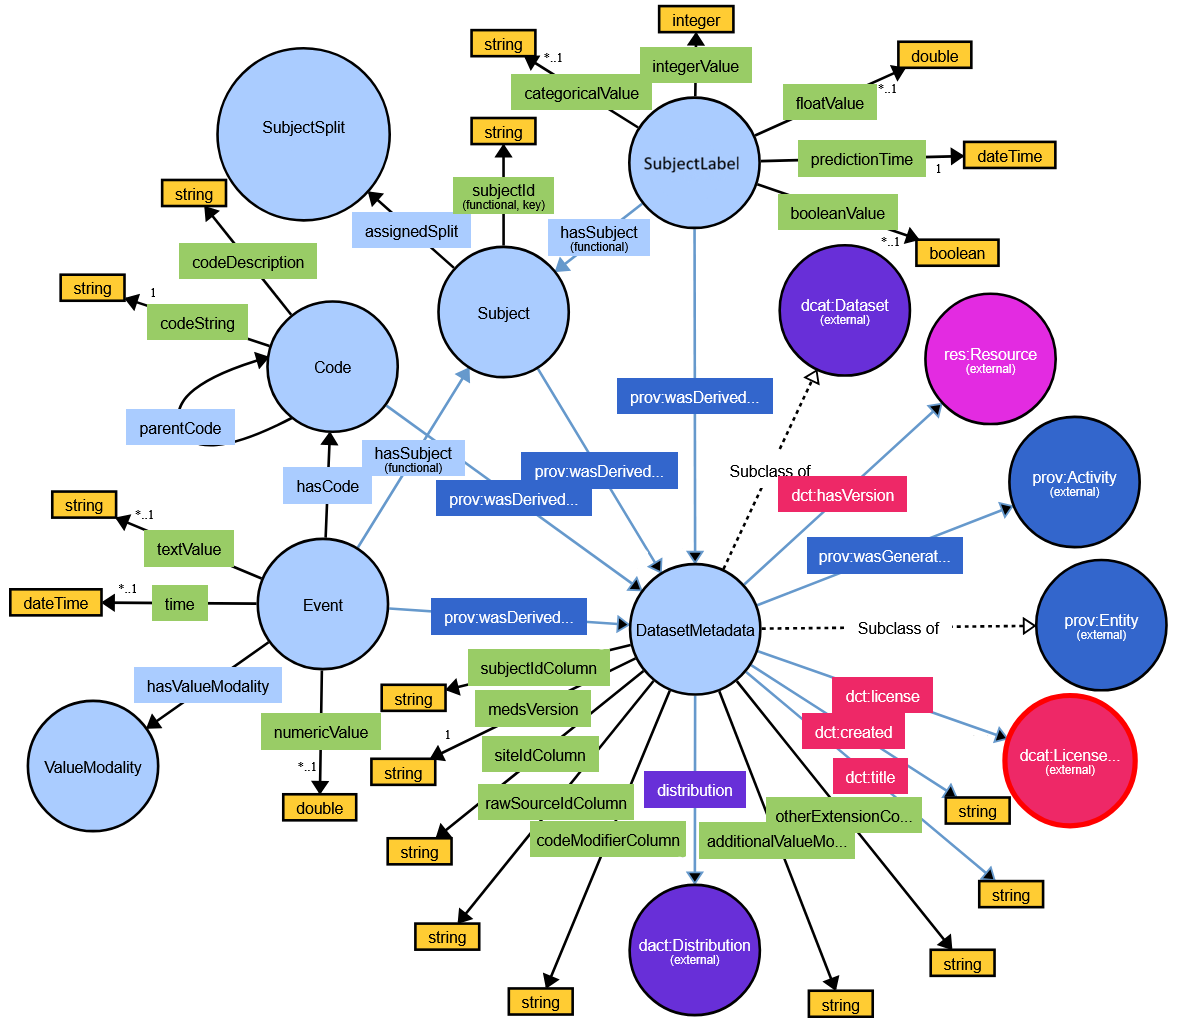
\includegraphics[width=\textwidth]{figures/paper3/fig1.png}
		\caption{Overview of the MEDS-OWL ontology. Azure nodes and edges denote locally defined classes and object properties, respectively. Black edges with green labels are datatype properties. Nodes and edges colored differently indicate imported entities from either the Data Catalogue Vocabulary (\texttt{dcat} prefix), Dublin Core Terms (\texttt{dct} prefix) or PROV-O (prefix \texttt{prov}). Dotted edges represent \texttt{subClassOf} predicate. The figure is drawn with WebVOWL.}%~\citep{lohmann_webvowl_2014}.}
	\label{fig:paper3_ontology-diagram}
\end{figure}

\begin{figure}[ht]
	\centering
	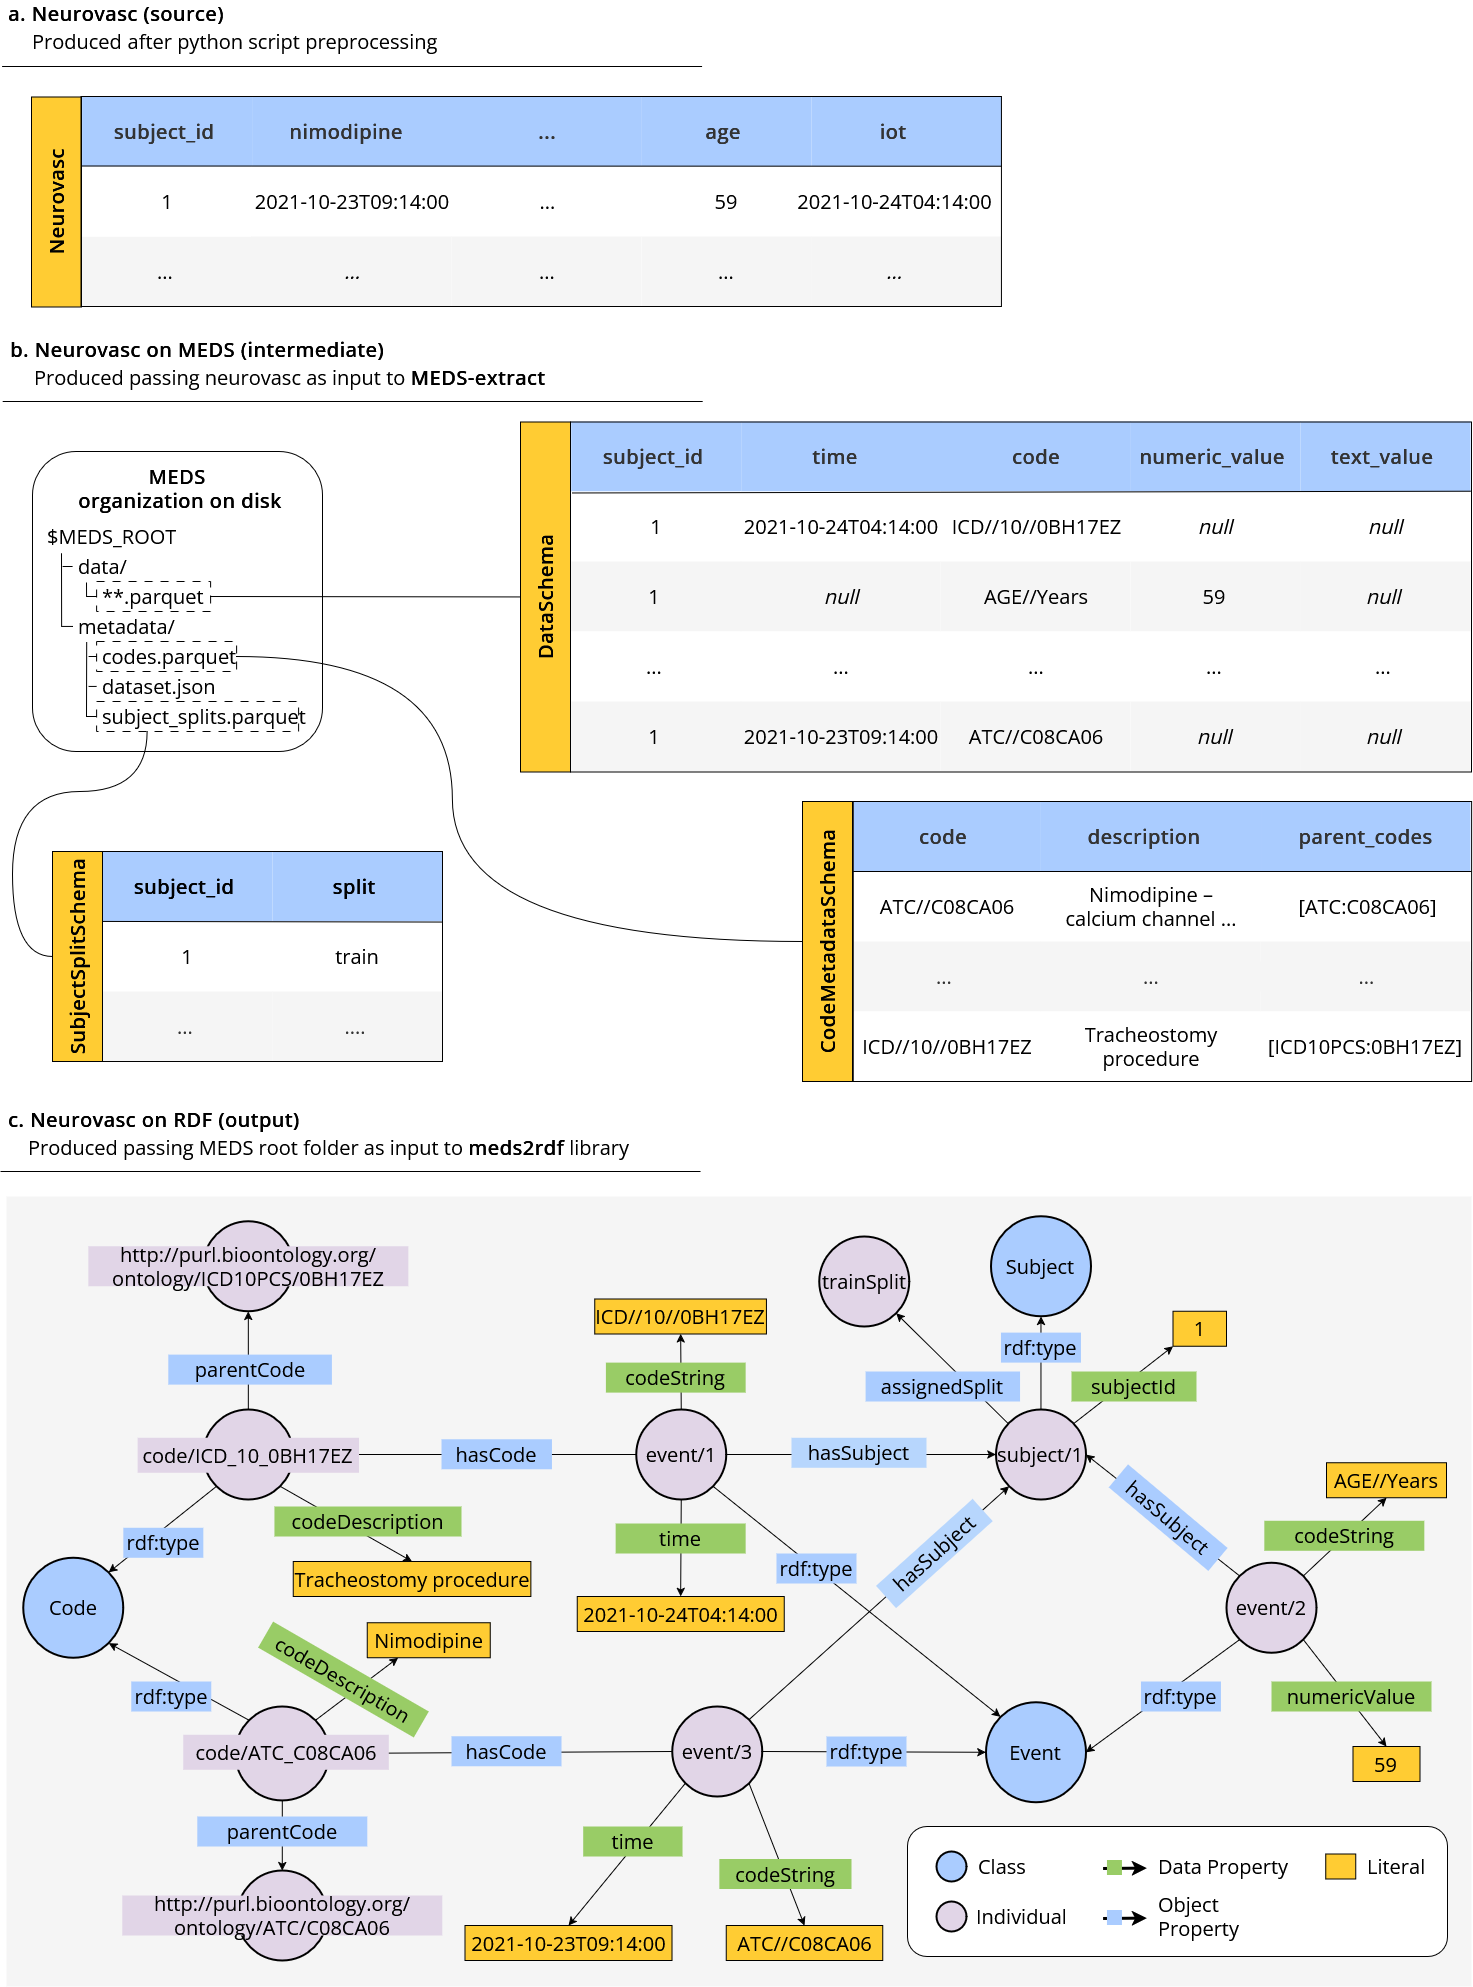
\includegraphics[width=\textwidth]{figures/paper3/fig2.png}
	\caption{MEDS-OWL conversion workflow for the NEUROVASC dataset. (a) Initial preprocessing of three patient features: age, nimodipine administration (ATC code: C08CA06), and tracheostomy procedure (ICD-10-PCS code: 0BH17EZ). (b) Conversion to MEDS tabular format via \texttt{MEDS-extract}, with each feature represented as a distinct event. (c) Transformation of the resulting MEDS dataset into MEDS-RDF using \texttt{meds2rdf}, which instantiates the corresponding MEDS-OWL classes.}
	\label{fig:paper3_etl-conversion}
\end{figure}

\begin{figure}[ht]
	\centering
	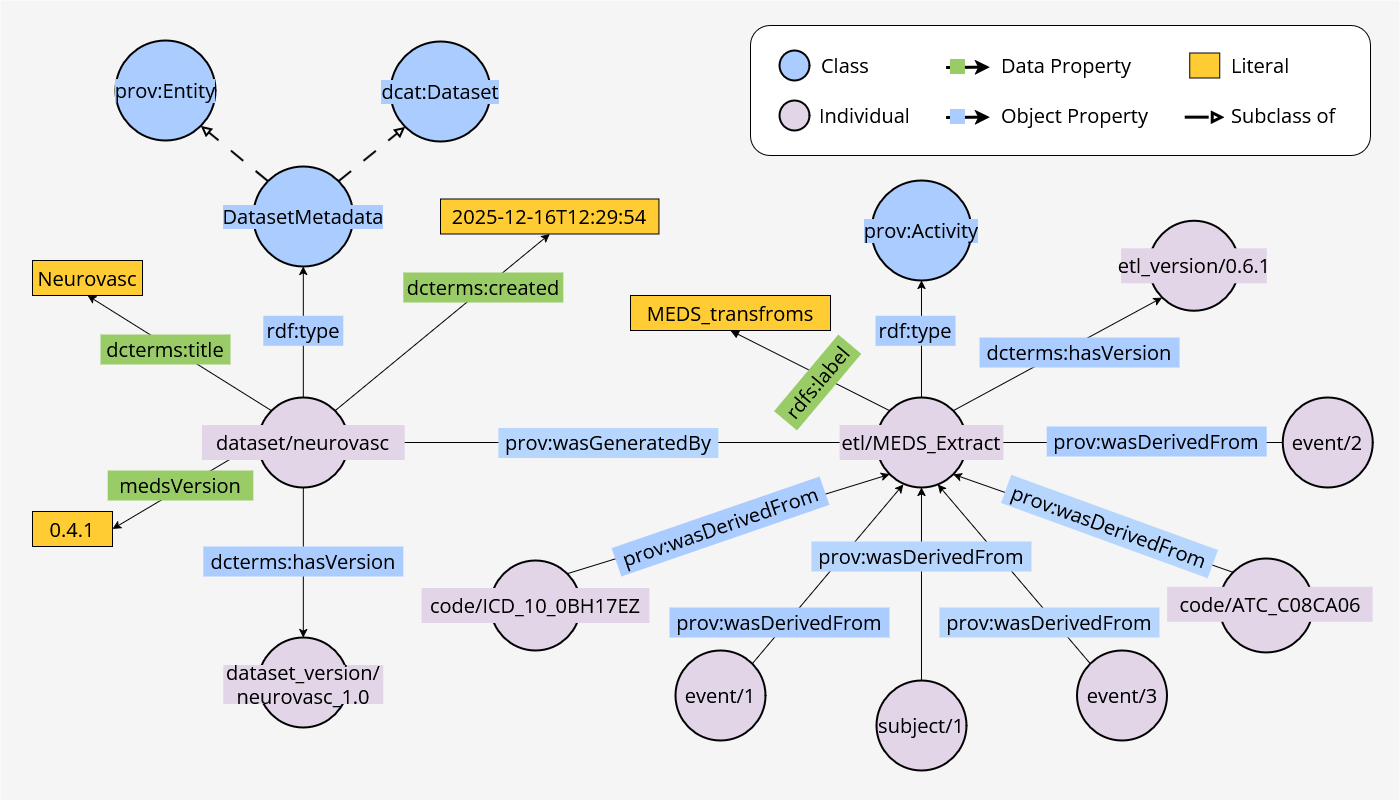
\includegraphics[width=\textwidth]{figures/paper3/fig3.png}
	\caption{Provenance linkage of MEDS events, codes, and subjects using MEDS-OWL, PROV-O, and Dublin Core. Each event references its source \texttt{meds:DatasetMetadata} instance (here, NEUROVASC) via \texttt{prov:wasDerivedFrom}; the dataset metadata records the creation time, MEDS schema version, and dataset title and is associated with the generating ETL activity (\texttt{prov:Activity}), here \texttt{MEDS-extract}.}
	\label{fig:paper3_provenance-instance}
\end{figure}

\begin{figure}[ht]
	\centering
	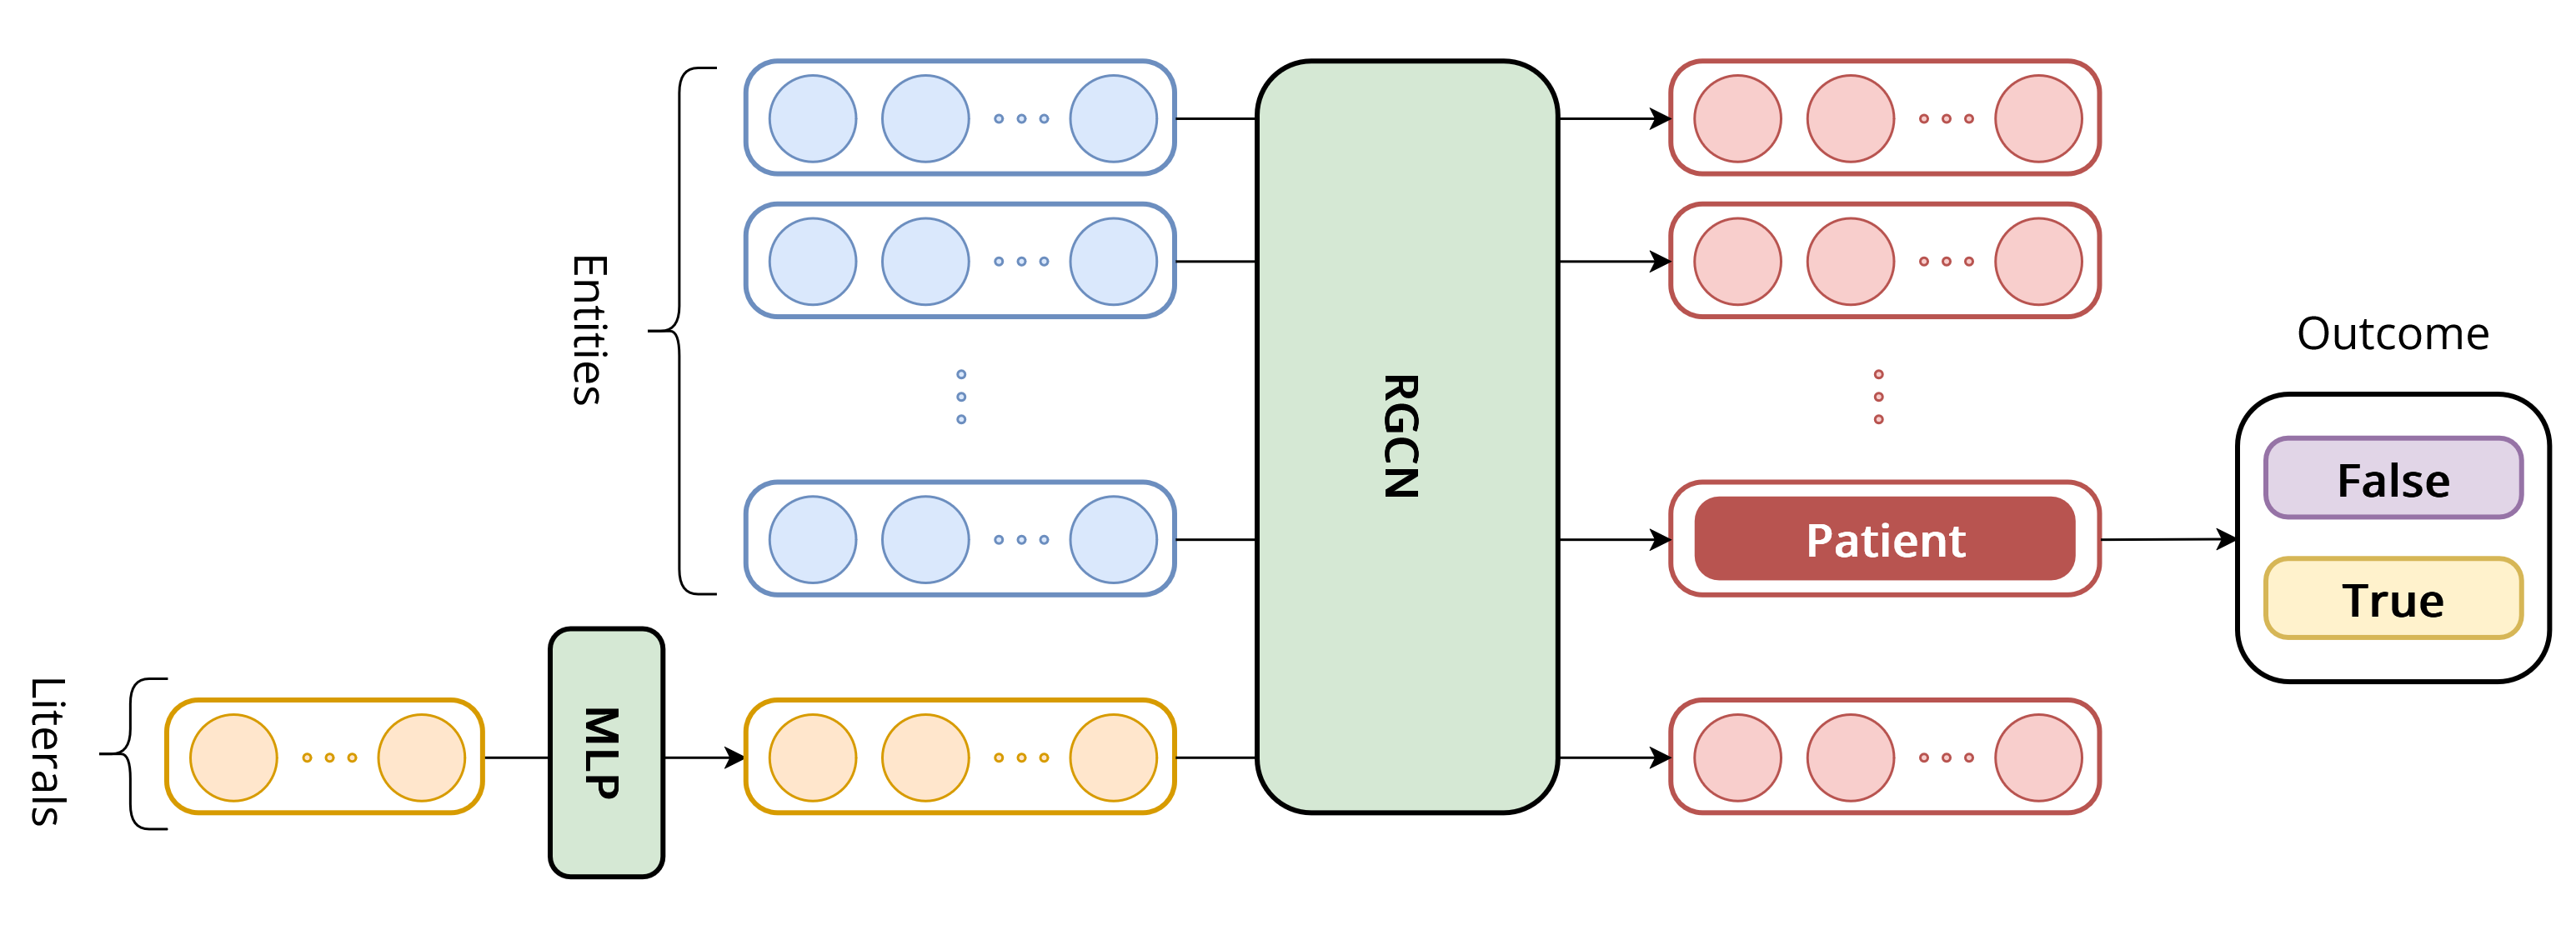
\includegraphics[width=\textwidth]{figures/paper3/fig4.png}
	\caption{Illustration of the RGCN+Lit model for patient outcome prediction.}
	\label{fig:paper3_rcgn+lit}
\end{figure}



%% ============================================================
\subsubsection{MEDS-OWL Mapping Tables}
\label{sec:paper3_supp-mapping-tables}
This section provides supplementary details on the MEDS-OWL ontology and
its correspondence with the MEDS schema. Table~\ref{tab:paper3_meds-owl-concepts}
summarizes the core MEDS-OWL classes, their intended meaning, and
representative examples. Table~\ref{tab:paper3_schema-to-ontology} provides a
high-level correspondence between the main MEDS schema components and the
MEDS-OWL classes used to represent them. The subsequent tables provide the
complete element-level mappings and the corresponding RDF triples:
Table~\ref{tab:paper3_events} details the mapping of the DataSchema elements to
\texttt{meds:Event} and \texttt{meds:Subject}; Table~\ref{tab:paper3_dataset}
details the mapping of DatasetMetadataSchema elements to
\texttt{meds:DatasetMetadata}; Table~\ref{tab:paper3_codes} reports the mapping of
CodeMetadataSchema elements to \texttt{meds:Code}; and
Table~\ref{tab:paper3_labels} reports the mappings of SubjectSplitSchema and
LabelSchema elements to \texttt{meds:SubjectSplit} and
\texttt{meds:SubjectLabel}, respectively.

\begin{table}[ht]
	\centering
	\caption{Core MEDS-OWL classes and their description, as defined by MEDS format.}
	\label{tab:paper3_meds-owl-concepts}
	\begin{tabular}{p{3.3cm} p{6.5cm} p{3.4cm}}
		\hline
		\textbf{Class} & \textbf{Description} & \textbf{Example} \\
		\hline
		\texttt{Subject} &
		Primary entity under observation, typically corresponding to a patient, admission, or longitudinal unit to which events are attributed. &
		Patient \#10234 \\
		\texttt{Event} &
		Atomic clinical observation or intervention representing a single MEDS row, characterized by a subject, a coded concept, and optional temporal and value attributes. &
		Administration of nimodipine at admission \\
		\texttt{Code} &
		An entity used to type events, which includes canonical identifiers, descriptions, and optional linkage to external terminologies or ontologies. &
		ATC:C08CA06 (Nimodipine) \\
		\texttt{DatasetMetadata} &
		Dataset-level description and provenance information, capturing identity, versioning, creation time, and ETL-related metadata. &
		X dataset, in MEDS format, v1.0 \\
		\texttt{SubjectSplit} &
		An assignment  of subjects to several disjoint sets aimed for an ML experiment. &
		Split for experiment 5 into a train, eval, and test sets\\
		\texttt{SubjectLabel} &
		A supervised learning instance defined by a subject identifier, an as-of prediction time (the latest time up to which subject data may be used for the prediction), and exactly one observed ground truth label value \(y\). &
		Subject \#10234, prediction time = discharge date, categorical label = rehabilitation\\
		\texttt{ValueModality} & Generic, extensible entity that links an \texttt{Event} to additional value modalities (for example, images, waveform recordings, audio clips, or other non-tabular payloads). & Chest X-ray image (DICOM series URI)\\
		\hline
	\end{tabular}
\end{table}

\begin{table}[ht]
	\centering
	\caption{Mapping from MEDS schema components to MEDS-OWL classes. See Table~\ref{tab:paper3_meds-owl-concepts} for class definitions and examples.}
	\label{tab:paper3_schema-to-ontology}
	\begin{tabular}{p{2.4cm} p{5.4cm} p{5.4cm}}
		\hline
		\textbf{MEDS schema} & \textbf{Brief description} & \textbf{Mapped MEDS-OWL class(es)} \\
		\hline
		DataSchema &
		Core medical event table describing sequences of subject events, where each row corresponds to a single clinical event. &
		\texttt{meds:Event} as the primary representation of each MEDS row from this table.  
		\texttt{meds:ValueModality} is used to model additional or non-tabular payloads associated with an event (e.g., images, waveforms, signals).  
		See Suppl. Table \ref{tab:paper3_events} for row-to-triple mappings. \\[4pt]%~\ref{tab:events}
		
		DatasetMetadata \\ Schema &
		Dataset-level metadata captures dataset identity, versioning, creation time, licensing, and ETL provenance information. &
		\texttt{meds:DatasetMetadata}, aligned with \texttt{dcterms} and \texttt{dcat}, and linked to ETL activities via \texttt{prov:wasGeneratedBy}.  
		See Suppl. Table \ref{tab:paper3_dataset}. \\[4pt] %~\ref{tab:dataset}
		
		CodeMetadata \\ Schema &
		Metadata describing the controlled vocabularies and codes used to type medical events, including canonical identifiers and hierarchical relations. &
		\texttt{meds:Code}, with \texttt{meds:codeString} as a canonical identifier and optional \texttt{meds:parentCode} relations to represent code hierarchies.  
		See Suppl. Table \ref{tab:paper3_codes}. \\[4pt] %~\ref{tab:codes}
		
		SubjectSplit \\ Schema &
		Specification of how subjects are assigned to disjoint subsets (e.g., for training, tuning, held-out) within a given supervised learning experiment. &
		\texttt{meds:SubjectSplit}, with subjects linked via \texttt{meds:assignedSplit}.  
		Multiple splits may coexist across experiments, while each subject belongs to exactly one subset per split.  
		See Suppl. Table \ref{tab:paper3_labels}. \\[4pt]%~\ref{tab:labels}
		
		LabelSchema &
		Definition of supervised learning labels associated with a subject at a specific prediction time, including the observed ground truth value. &
		\texttt{meds:SubjectLabel}, capturing the prediction cutoff time (\texttt{meds:predictionTime}) and exactly one label value using datatype-specific properties.  
		See Suppl. Table \ref{tab:paper3_labels}. \\[4pt] %~\ref{tab:labels}
		
		(subject identifier) &
		Subject identifiers appear across multiple MEDS schemas and provide the logical join key between events, splits, and labels. &
		\texttt{meds:Subject}, representing the canonical subject entity via \texttt{meds:subjectId}, and serving as the hub linking \texttt{Event}, \texttt{SubjectLabel}, and \texttt{SubjectSplit}. \\
		
		\hline
	\end{tabular}
\end{table}

\begin{table}[ht]
	\centering
	\caption{Mapping of the elements of the MEDS DataSchema tables to \texttt{meds:Event} and \texttt{meds:Subject} classes, with descriptions. For each tuple (or row) of DataSchema, a list of associated RDF triples is generated. Card. stands for the cardinality of the relationship.}
	\label{tab:paper3_events}
	\begin{tabular}{l p{4.8cm} >{\raggedright}p{3.8cm} c}
		\hline
		\textbf{MEDS element} & \textbf{Description} & \textbf{RDF triple} & \textbf{Card.} \\
		\hline
		event\_row e & The row representing an event e of the subject s. & \texttt{?e a meds:Event.}  & 1 \\
		subject\_id id& The identifier of the subject s (typically the patient). & \texttt{?s a meds:Subject. \break ?s meds:subjectId ?id}\verb|^^|\texttt{xsd:string.} \break \texttt{?e meds:hasSubject ?s.} & 1 \\
		time t& The time of the measurement, nullable for static measurements. & \texttt{?e meds:time ?t}\verb|^^|\texttt{xsd:dateTime.} & 0..1 \\
		code c & The categorical descriptor of the measurement (e.g., lab test, diagnosis code). & \texttt{?c a meds:Code. \break ?e meds:hasCode ?c.} & 1 \\
		code\_string cs& The string representation of the code. & \texttt{?e meds:codeString ?cs.}\verb|^^|\texttt{xsd:string.} & 1 \\
		numeric\_value nv & A numeric value associated with the measurement (e.g., lab test result), nullable. & \texttt{?e meds:numericValue ?nv}\verb|^^|\texttt{xsd:double.} & 0..1 \\
		text\_value tv & A text value associated with the measurement (e.g., clinical note, text-based test result), nullable. & \texttt{?e meds:textValue ?tv}\verb|^^|\texttt{xsd:string.} & 0..1 \\
		\hline
	\end{tabular}
\end{table}
%
\begin{table}[ht]
	\centering
	\caption{Mapping metadata of a transformed MEDS dataset (DatasetMetadataSchema) to the \texttt{meds:DatasetMetadata} class. For each dataset generated, a list of associated ``meta'' RDF triples is generated.}
	\label{tab:paper3_dataset}
	\begin{tabular}{l p{3.8cm} >{\raggedright}p{4.6cm} c}
		\hline
		\textbf{MEDS element} & \textbf{Description} & \textbf{RDF triple} & \textbf{Card.} \\
		\hline
		dataset ds & The dataset converted to RDF. & \texttt{?ds a meds:DatasetMetadata.%\break rdfs:subClassOf prov:Entity, dcat:Dataset.
		} & 1 \\
		dataset\_name n & The name of the dataset ds. & \texttt{?ds dct:title ?n}\verb|^^|\texttt{xsd:string.} & 1 \\
		dataset\_version dsv& The version of the dataset. & \texttt{?ds dct:hasVersion ?dsv.} & 0..1 \\
		meds\_version mv& The version of the MEDS schema. & \texttt{?ds meds:medsVersion ?mv}\verb|^^|\texttt{xsd:string.} & 1 \\
		created\_at & ISO 8601 creation date and time. & \texttt{?ds dct:created ?time}\verb|^^|\texttt{xsd:dateTime.} & 1 \\
		license & License under which the dataset is released. & \texttt{?li a dct:LicenseDocument. \break ?ds dct:license ?li.} & 0..1 \\
		location\_uri & URI(s) where the dataset is hosted. & \texttt{?ds dcat:distribution ?dist. \break ?dist dcat:downloadURL ?dw.} & 0..* \\
		description\_uri & URI(s) referencing a detailed description of the dataset. & \texttt{?dist dcat:accessURL ?au.} & 0..* \\
		etl\_name etln& Name of the ETL process etl that generated the dataset. & \texttt{?etl a prov:Activity. \break ?etl rdfs:label ?etln. \break ?ds prov:wasGeneratedBy ?etl.} & 0..1 \\
		etl\_version etlv& Version of the ETL process. & 
		\texttt{?etl dct:hasVersion ?etlv.} & 0..1 \\
		\hline
	\end{tabular}
\end{table}
%
\begin{table}[ht]
	\centering
	\caption{Mapping of the elements of the MEDS CodeMetadataSchema table to \texttt{meds:Code} class. For each tuple (or row) of CodeMetadataSchema, a list of associated RDF triples is generated. } 
	\label{tab:paper3_codes}
	\begin{tabular}{l p{4.2cm} >{\raggedright}p{4.5cm} c}
		\hline
		\textbf{MEDS element} & \textbf{Description} & \textbf{RDF triple} & \textbf{Card.} \\
		\hline
		code\_row c & The row representing a code c in the dataset. & \texttt{?c a meds:Code.} & 1 \\
		code\_string cs & The categorical descriptor of a possible measurement; links to the DataSchema code column. & \texttt{?c meds:codeString ?cs}\verb|^^|\texttt{xsd:string.} & 1 \\
		description d& A human-readable description of what the code represents. & \texttt{?c meds:codeDescription ?d}\verb|^^|\texttt{xsd:string.} & 0..1 \\
		parent\_codes p & One or more higher-level or parent codes in an ontological hierarchy, possibly linking to other codes in MEDS or external vocabularies (e.g., OMOP CDM). & \texttt{?p a meds:Code. \break ?c meds:parentCode ?p.} & 0..* \\
		\hline
	\end{tabular}
\end{table}
%
\begin{table}[ht]
	\centering
	\caption{Mapping of the elements of MEDS SubjectSplitSchema and LabelSchema tables to \texttt{meds:SubjectSplit} and \texttt{meds:SubjectLabel} classes, respectively. For each tuple (or row) of LabelSchema, a list of associated RDF triples is generated.
	}
	\label{tab:paper3_labels}
	\begin{tabular}{l >{\raggedright}p{4.2cm} >{\raggedright}p{4.5cm} c}
		\hline
		\textbf{MEDS element} & \textbf{Description} & \textbf{RDF triple} & \textbf{Card.} \\
		\hline
		split & The name of the subset a subject is assigned to, following a dataset split (e.g., train, validation, test). & \texttt{?set a meds:SubjectSplit. \break ?s a meds:Subject. \break ?s meds:assignedSplit ?set.} & 0..* \\
		
		label\_row & A prediction label (sample) for a subject in a supervised learning task. This is the ground truth label extracted from the dataset according to the task specification. & \texttt{?l a meds:SubjectLabel. \break ?l meds:hasSubject ?s.} & 0..* \\
		
		prediction\_time & The timestamp representing the endpoint of the data that can be used to predict the label for the given sample. This is not necessarily the time of the event itself nor the deployment prediction time. It defines the "as-of" cutoff for input data. & \texttt{?l meds:predictionTime ?pt}\verb|^^|\texttt{xsd:dateTime.} & 1 \\
		
		label\_value & The value for the label. It can be one of the following types depending on the task: binary tasks, ordinal or continuous numeric tasks, and categorical tasks. 
		&
		\texttt{?l meds:booleanValue ?bv}\verb|^^|\texttt{xsd:boolean.} \break
		\texttt{?l meds:integerValue ?iv}\verb|^^|\texttt{xsd:integer.} \break
		\texttt{?l meds:floatValue ?fv}\verb|^^|\texttt{xsd:double.} \break
		\texttt{?l meds:categoricalValue ?cv}\verb|^^|\texttt{xsd:string.} & 0..1 \\
		\hline
	\end{tabular}
\end{table}

%% ============================================================

%\section{Supplementary Methods}

\subsubsection{Round-Trip Fidelity Evaluation}\label{sec:paper3_supp-fidelity}
To assess whether the MEDS-RDF transformation preserves information faithfully, %, beyond the structural statistics reported in Section~\ref{sec:usage-examples},
we conducted a \emph{round-trip fidelity} evaluation across all four datasets previously described. For each dataset, we (\textit{i}) converted a sample of MEDS events to RDF using \texttt{meds2rdf}, (\textit{ii}) reconstructed a tabular representation from the resulting RDF graph, and (\textit{iii}) compared the reconstructed data with the original MEDS source along several dimensions.

\paragraph{Sampling strategy.}
Because several datasets are too large to process exhaustively on a single workstation, we performed $K = 5$ independent random samples per dataset. Each sample $k \in \{1, \ldots, K\}$ was drawn by selecting $N = 100$ patients uniformly at random without replacement, retaining all events associated with those patients. Let $\mathcal{D}_k^{\text{orig}}$ and $\mathcal{D}_k^{\text{recon}}$ denote the sets of events in the original and reconstructed samples, respectively, and let $\mathcal{S}_k^{\text{orig}}$, $\mathcal{S}_k^{\text{recon}}$ denote the corresponding subject sets. For each scalar metric $m$, we report the sample mean $\bar{m} = \frac{1}{K}\sum_{k=1}^{K} m_k$. For the numeric null-rate, where within-dataset variability is clinically meaningful, we additionally report the sample standard deviation $\sigma_m = \sqrt{\frac{1}{K-1}\sum_{k=1}^{K}(m_k - \bar{m})^2}$.

\paragraph{Metrics.}
Let $f \in \{$\texttt{subject\_id}, \texttt{code}, \texttt{time}, \texttt{numeric\_value}, \texttt{text\_value}$\}$ denote a MEDS field, and let $e_i^{\text{orig}}$, $e_i^{\text{recon}}$ denote the values of field $f$ for event $i$ in the original and reconstructed datasets, respectively. We define the following metrics for sample $k$:

\begin{itemize}
	
	\item \emph{Structural completeness}:
	\[
	C_{\text{struct}} = \frac{|\mathcal{D}_k^{\text{recon}}|}{|\mathcal{D}_k^{\text{orig}}|}
	\]
	the proportion of original events successfully recovered after round-trip conversion.
	
	\item \emph{Subject completeness}:
	\[
	C_{\text{subj}} = \frac{|\mathcal{S}_k^{\text{recon}}|}{|\mathcal{S}_k^{\text{orig}}|}
	\]
	the proportion of original subjects whose events appear in the reconstructed dataset.
	
	\item \emph{Field-level fidelity} for field $f$, computed over the $n$ uniquely joinable event pairs:
	\[
	F_f = \frac{1}{n} \sum_{i=1}^{n} \mathbf{1}\!\left[e_i^{\text{recon}} = e_i^{\text{orig}}\right]
	\]
	the exact-match rate. Events with duplicate composite keys $(\texttt{subject\_id}, \texttt{time}, \texttt{code})$ cannot be uniquely matched and are excluded from this metric; their fidelity is assessed separately via approximate matching.
	
	\item \emph{Numeric precision} for \texttt{numeric\_value}, computed over non-null value pairs:
	\[
	\varepsilon_{\max} = \max_i \left| e_i^{\text{recon}} - e_i^{\text{orig}} \right|, \qquad
	\bar{\varepsilon} = \frac{1}{n} \sum_{i=1}^{n} \left| e_i^{\text{recon}} - e_i^{\text{orig}} \right|
	\]
	and the 99th-percentile relative error: \break $\varepsilon_{99} = \operatorname{Quantile}_{0.99}\!\left(\frac{|e_i^{\text{recon}} - e_i^{\text{orig}}|}{|e_i^{\text{orig}}| + \epsilon}\right)$, where $\epsilon = 10^{-9}$ avoids division by zero.
	
	\item \emph{Temporal precision} for \texttt{time}, expressed in seconds:
	\[
	\delta_{\max} = \max_i \left| t_i^{\text{recon}} - t_i^{\text{orig}} \right|_{\text{s}}, \qquad
	\bar{\delta} = \frac{1}{n} \sum_{i=1}^{n} \left| t_i^{\text{recon}} - t_i^{\text{orig}} \right|_{\text{s}}
	\]
	
	\item \emph{Code and split completeness}:
	\[
	C_{\text{code}} = \frac{|\mathcal{C}^{\text{recon}}|}{|\mathcal{C}^{\text{orig}}|}, \qquad
	C_{\text{split}} = \frac{|\mathcal{P}^{\text{recon}}|}{|\mathcal{P}^{\text{orig}}|}
	\]
	where $\mathcal{C}$ and $\mathcal{P}$ denote the sets of distinct codes and split assignments, respectively.
\end{itemize}

\subsubsection{MEDS-RDF Transformation Examples}
\label{sec:paper3_supp-transformation-examples}
% To ground the formal model in practice, we now illustrate the full transformation pipeline from raw clinical data to RDF graphs. We use two datasets, NEUROVASC and MIMIC-IV, chosen to contrast a controlled synthetic cohort with a large-scale real-world EHR dataset.

\paragraph{NEUROVASC example}
The NEUROVASC dataset provides a compact setting for illustrating the full MEDS-RDF pipeline. Each patient is represented by 30 clinical features, including 8 time-stamped events representing the interval from hospital admission to their first occurrence, and 22 non-temporal demographic or historical features. Patient outcomes are categorized in one of three values: Back Home, Rehabilitation, or Death, depending on the patient's status at the end of the hospital stay. %The dataset preserves realistic correlations and event transitions, making it suitable for testing ontology-driven data representation of clinical pathways and basic analytics. 
The complete NEUROVASC transformation workflow is illustrated in Suppl. Figure~\ref{fig:paper3_etl-conversion}, while the corresponding provenance representation is provided in Suppl. Figure~\ref{fig:paper3_provenance-instance}.

The subsequent conversion of MEDS events into RDF using the \texttt{meds2rdf} library results in a KG comprising 1,330,351 RDF triples. The graph contains 255,135 distinct subjects, 18 predicates, and 46,722 distinct objects, corresponding to 255,161 distinct IRIs and 36,594 literals, with no blank nodes generated. In terms of instantiated ontology elements, the graph includes 245,015 individuals of class \texttt{meds:Event}, corresponding one-to-one with the MEDS events, as well as 10,000 \texttt{meds:Subject} instances and 115 \texttt{meds:Code} instances reused across events. Dataset-level metadata is represented by a single \texttt{meds:DatasetMetadata} individual, while three predefined \texttt{meds:SubjectSplit} individuals capture the train, validation, and test partitions. No label instances are generated for this dataset, as outcome labels are not represented in the current transformation.

Finally, we analyzed the structural footprint of events in the resulting RDF graph. Each \texttt{meds:Event} node is described, on average, by 5.31 RDF triples (standard deviation 0.46), with a minimum of 5 and a maximum of 6 triples per event. This low variance reflects the regular structure imposed by MEDS-OWL cardinality constraints, where subject and code associations are mandatory, while temporal and value-related properties are optional. These statistics demonstrate that the transformation produces a compact RDF representation of events while preserving semantic richness and provenance information.

\paragraph{MIMIC-IV example of usage} To further demonstrate the applicability of \texttt{meds2rdf} to real-world EHRs at a level of detail comparable to the NEUROVASC example above, we applied the library to the publicly available \textit{MIMIC-IV demo} dataset, a fixed, pre-defined 100-patient subset of MIMIC-IV already formatted in MEDS. We use this small, openly accessible demo specifically for this illustrative example, as it keeps the workflow tractable for visualization and reproducibility. %The round-trip fidelity and scalability evaluations reported in Sections~\ref{sec:fidelity} and \ref{sec:scalability} instead use the full MIMIC-IV dataset, and are therefore not directly comparable to the statistics reported below.

The conversion generated 916,166 MEDS events distributed across the ML splits as follows: 803,992 in the train set, 69,620 in the tuning set, and 42,554 in the held-out set. The resulting KG comprises 6,408,529 RDF triples, including 925,706 distinct subjects, 19 predicates, 126,680 distinct objects, 925,733 distinct IRIs, and 117,132 literals, with no blank nodes generated. Ontology instantiation includes 916,166 individuals of class \texttt{meds:Event}, 100 \texttt{meds:Subject} individuals, 9,435 \texttt{meds:Code} individuals, three \texttt{meds:SubjectSplit} individuals, and one \texttt{meds:DatasetMetadata} individual. No label or \texttt{ValueModality} instances were included in this subset. Each \texttt{meds:Event} in the MIMIC-IV subset is represented by an average of 6.97 RDF triples (median 7.0, minimum 5, maximum 8, standard deviation 0.42), indicating a slightly richer structure per event compared to NEUROVASC, due to the higher number of numeric and text values associated with MIMIC events. As with the NEUROVASC example, this conversion used the \texttt{GraphSink} strategy. %Together, these two usage examples confirm that \texttt{meds2rdf} preserves the semantic and provenance structure defined by MEDS-OWL; the next two subsections evaluate this preservation, and the computational cost of achieving it, systematically and at scale across all four datasets.

\subsubsection{Full Prediction Task Results}
\label{sec:paper3_supp-results}

This section reports the complete per-task results. Table~\ref{tab:paper3_results-schema-full} reports the full schema-granularity progression (MEDS-RDF-Base, -Partial, and -Full) across all 11 MIMIC-IV prediction tasks, considering both the entire (unpruned) dataset and the SHAP-pruned subset. Table~\ref{tab:paper3_rgcn-depth} reports the sensitivity of predictive performance and computational cost to increasing the RGCN depth from two to five layers. Table~\ref{tab:paper3_results-tabular-full} reports the complete comparison of RGCN2+lit (MEDS-RDF-Full, SHAP-pruned) with the three tabular baselines (Logistic Regression, Random Forest, and XGBoost) across all 11 tasks. Finally, Table~\ref{tab:paper3_results-xgb-statistical} provides the subsample-level Macro-F1 results for RGCN+lit and XGBoost, together with the paired differences and statistical significance of their performance differences across the five patient subsamples for each task.

% Please add the following required packages to your document preamble:
% \usepackage{multirow}
% \usepackage{graphicx}
\begin{table}[ht]
	\caption{Schema-granularity progression across MIMIC-IV tasks. \emph{Entire} denotes the unpruned dataset; \emph{Only top 10\%} denotes the subset retaining the top 10\% of relations by SHAP importance. \emph{Base}, \emph{Partial}, and \emph{Full} denote the corresponding MEDS-RDF schema variants. The winning schema per task is shown in bold.}
	\label{tab:paper3_results-schema-full}
	\resizebox{\textwidth}{!}{%
		\begin{tabular}{lllcccccc}
			\hline
			\multicolumn{1}{c}{\multirow{4}{*}{Task}} & \multicolumn{1}{c}{\multirow{4}{*}{Dataset}} & \multicolumn{1}{c}{\multirow{4}{*}{\begin{tabular}[c]{@{}c@{}}Schema\end{tabular}}} & \multicolumn{3}{c}{\multirow{2}{*}{F1-score}} & \multirow{4}{*}{Accuracy} & \multirow{4}{*}{AUC} & \multirow{4}{*}{AUPRC} \\
			\multicolumn{1}{c}{} & \multicolumn{1}{c}{} & \multicolumn{1}{c}{} & \multicolumn{3}{c}{} &  &  &  \\ \cline{4-6}
			\multicolumn{1}{c}{} & \multicolumn{1}{c}{} & \multicolumn{1}{c}{} & \multirow{2}{*}{False} & \multirow{2}{*}{True} & \multirow{2}{*}{Macro} &  &  &  \\
			\multicolumn{1}{c}{} & \multicolumn{1}{c}{} & \multicolumn{1}{c}{} &  &  &  &  &  &  \\ \hline
			\multirow{5}{*}{\begin{tabular}[c]{@{}l@{}}First 24h \\ in-hospital\\ mortality\end{tabular}} & \multirow{2}{*}{Entire} & Base & 0.61 ± 0.06 & 0.63 ± 0.12 & 0.62 ± 0.08 & 0.61 ± 0.06 & 0.66 ± 0.07 & 0.67 ± 0.07 \\
			&  & Partial & 0.66 ± 0.05 & 0.66 ± 0.06 & 0.66 ± 0.05 & 0.65 ± 0.04 & 0.73 ± 0.05 & 0.72 ± 0.06 \\ \cline{2-9} 
			& \multirow{3}{*}{\begin{tabular}[c]{@{}l@{}}Only \\ top 10\%\end{tabular}} & Base & 0.54 ± 0.15 & 0.57 ± 0.16 & 0.56 ± 0.12 & 0.56 ± 0.06 & 0.59 ± 0.09 & 0.60 ± 0.08 \\
			&  & Partial & 0.64 ± 0.06 & 0.62 ± 0.05 & 0.63 ± 0.05 & 0.63 ± 0.05 & 0.69 ± 0.06 & 0.67 ± 0.06 \\
			&  & Full & \textbf{0.73 ± 0.05} & \textbf{0.71 ± 0.05} & \textbf{0.72 ± 0.04} & \textbf{0.72 ± 0.05} & \textbf{0.80 ± 0.05} & \textbf{0.79 ± 0.05} \\ \hline
			\multirow{5}{*}{\begin{tabular}[c]{@{}l@{}}First 24h \\ in-ICU\\ mortality\end{tabular}} & \multirow{2}{*}{Entire} & Base & 0.34 ± 0.25 & 0.38 ± 0.22 & 0.36 ± 0.13 & 0.50 ± 0.04 & 0.52 ± 0.07 & 0.53 ± 0.05 \\
			&  & Partial & 0.60 ± 0.05 & 0.60 ± 0.06 & 0.60 ± 0.05 & 0.59 ± 0.05 & 0.64 ± 0.07 & 0.65 ± 0.06 \\ \cline{2-9} 
			& \multirow{3}{*}{\begin{tabular}[c]{@{}l@{}}Only \\ top 10\%\end{tabular}} & Base & 0.42 ± 0.23 & 0.31 ± 0.27 & 0.37 ± 0.16 & 0.50 ± 0.02 & 0.50 ± 0.06 & 0.51 ± 0.05 \\
			&  & Partial & 0.58 ± 0.06 & 0.57 ± 0.13 & 0.58 ± 0.08 & 0.57 ± 0.05 & 0.62 ± 0.06 & 0.62 ± 0.07 \\
			&  & Full & \textbf{0.74 ± 0.06} & \textbf{0.74 ± 0.05} & \textbf{0.74 ± 0.05} & \textbf{0.74 ± 0.04} & \textbf{0.82 ± 0.05} & \textbf{0.80 ± 0.05} \\ \hline
			\multirow{5}{*}{\begin{tabular}[c]{@{}l@{}}First 48h \\ in-hospital\\ mortality\end{tabular}} & \multirow{2}{*}{Entire} & Base & 0.45 ± 0.22 & 0.50 ± 0.20 & 0.48 ± 0.16 & 0.53 ± 0.06 & 0.55 ± 0.08 & 0.58 ± 0.07 \\
			&  & Partial & 0.67 ± 0.06 & 0.67 ± 0.06 & 0.67 ± 0.05 & 0.66 ± 0.05 & 0.72 ± 0.06 & 0.71 ± 0.07 \\ \cline{2-9} 
			& \multirow{3}{*}{\begin{tabular}[c]{@{}l@{}}Only \\ top 10\%\end{tabular}} & Base & 0.55 ± 0.20 & 0.46 ± 0.23 & 0.51 ± 0.17 & 0.55 ± 0.06 & 0.57 ± 0.10 & 0.58 ± 0.08 \\
			&  & Partial & 0.65 ± 0.05 & 0.64 ± 0.06 & 0.65 ± 0.04 & 0.64 ± 0.04 & 0.70 ± 0.05 & 0.70 ± 0.06 \\
			&  & Full & \textbf{0.74 ± 0.06} & \textbf{0.72 ± 0.06} & \textbf{0.73 ± 0.05} & \textbf{0.73 ± 0.05} & \textbf{0.80 ± 0.05} & \textbf{0.79 ± 0.07} \\ \hline
			\multirow{5}{*}{\begin{tabular}[c]{@{}l@{}}First 48h \\ in-ICU\\ mortality\end{tabular}} & \multirow{2}{*}{Entire} & Base & 0.45 ± 0.19 & 0.49 ± 0.32 & 0.47 ± 0.19 & 0.52 ± 0.03 & 0.52 ± 0.06 & 0.54 ± 0.05 \\
			&  & Partial & 0.62 ± 0.05 & 0.63 ± 0.06 & 0.63 ± 0.04 & 0.62 ± 0.04 & 0.66 ± 0.05 & 0.66 ± 0.05 \\ \cline{2-9} 
			& \multirow{3}{*}{\begin{tabular}[c]{@{}l@{}}Only \\ top 10\%\end{tabular}} & Base & 0.44 ± 0.27 & 0.57 ± 0.22 & 0.51 ± 0.19 & 0.56 ± 0.08 & 0.57 ± 0.10 & 0.58 ± 0.09 \\
			&  & Partial & 0.61 ± 0.08 & 0.61 ± 0.07 & 0.61 ± 0.06 & 0.60 ± 0.05 & 0.65 ± 0.06 & 0.66 ± 0.06 \\
			&  & Full & \textbf{0.74 ± 0.05} & \textbf{0.74 ± 0.06} & \textbf{0.74 ± 0.05} & \textbf{0.74 ± 0.05} & \textbf{0.82 ± 0.05} & \textbf{0.81 ± 0.06} \\ \hline
			\multirow{5}{*}{\begin{tabular}[c]{@{}l@{}}LOS in ICU \\ \textgreater 3 days\end{tabular}} & \multirow{2}{*}{Entire} & Base & 0.72 ± 0.13 & 0.79 ± 0.14 & 0.76 ± 0.12 & 0.76 ± 0.07 & 0.84 ± 0.06 & 0.86 ± 0.06 \\
			&  & Partial & 0.59 ± 0.08 & 0.59 ± 0.10 & 0.59 ± 0.09 & 0.59 ± 0.08 & 0.62 ± 0.11 & 0.63 ± 0.10 \\ \cline{2-9} 
			& \multirow{3}{*}{\begin{tabular}[c]{@{}l@{}}Only \\ top 10\%\end{tabular}} & Base & 0.58 ± 0.29 & 0.70 ± 0.25 & 0.64 ± 0.24 & 0.69 ± 0.14 & 0.74 ± 0.16 & 0.77 ± 0.16 \\
			&  & Partial & 0.68 ± 0.08 & 0.67 ± 0.10 & 0.68 ± 0.08 & 0.67 ± 0.09 & 0.73 ± 0.09 & 0.73 ± 0.09 \\
			&  & Full & \textbf{0.83 ± 0.04} & \textbf{0.83 ± 0.05} & \textbf{0.83 ± 0.04} & \textbf{0.83 ± 0.04} & \textbf{0.91 ± 0.03} & \textbf{0.91 ± 0.03} \\ \hline
			\multirow{5}{*}{\begin{tabular}[c]{@{}l@{}}LOS \\ in Hospital \\ \textgreater 3 days\end{tabular}} & \multirow{2}{*}{Entire} & Base & 0.73 ± 0.05 & 0.81 ± 0.05 & 0.77 ± 0.04 & 0.76 ± 0.04 & 0.84 ± 0.04 & 0.85 ± 0.04 \\
			&  & Partial & 0.99 ± 0.01 & 0.99 ± 0.01 & 0.99 ± 0.01 & 0.99 ± 0.01 & 0.99 ± 0.01 & 1.00 ± 0.01 \\ \cline{2-9} 
			& \multirow{3}{*}{\begin{tabular}[c]{@{}l@{}}Only \\ top 10\%\end{tabular}} & Base & 0.72 ± 0.06 & 0.82 ± 0.06 & 0.77 ± 0.04 & 0.75 ± 0.05 & 0.84 ± 0.04 & 0.85 ± 0.05 \\
			&  & Partial & 0.99 ± 0.01 & 0.99 ± 0.02 & 0.99 ± 0.01 & 0.99 ± 0.01 & 1.00 ± 0.01 & 1.00 ± 0.00 \\
			&  & Full & \textbf{0.99 ± 0.01} & \textbf{1.00 ± 0.01} & \textbf{0.99 ± 0.01} & \textbf{0.99 ± 0.01} & \textbf{1.00 ± 0.01} & \textbf{1.00 ± 0.00} \\ \hline
			\multirow{5}{*}{\begin{tabular}[c]{@{}l@{}}1y \\ post-hospital- \\discharge \\ mortality\end{tabular}} & \multirow{2}{*}{Entire} & Base & 0.67 ± 0.07 & 0.63 ± 0.15 & 0.65 ± 0.10 & 0.64 ± 0.06 & 0.71 ± 0.06 & 0.70 ± 0.06 \\
			&  & Partial & 0.76 ± 0.06 & 0.73 ± 0.05 & 0.74 ± 0.04 & 0.74 ± 0.04 & 0.82 ± 0.04 & 0.81 ± 0.05 \\ \cline{2-9} 
			& \multirow{3}{*}{\begin{tabular}[c]{@{}l@{}}Only \\ top 10\%\end{tabular}} & Base & 0.63 ± 0.16 & 0.63 ± 0.09 & 0.63 ± 0.11 & 0.61 ± 0.08 & 0.68 ± 0.09 & 0.71 ± 0.06 \\
			&  & Partial & 0.77 ± 0.05 & 0.74 ± 0.05 & 0.76 ± 0.04 & 0.75 ± 0.05 & 0.84 ± 0.04 & 0.83 ± 0.05 \\
			&  & Full & \textbf{0.82 ± 0.05} & \textbf{0.80 ± 0.06} & \textbf{0.81 ± 0.05} & \textbf{0.81 ± 0.05} & \textbf{0.89 ± 0.04} & \textbf{0.89 ± 0.04} \\ \hline
			\multirow{5}{*}{\begin{tabular}[c]{@{}l@{}}30d \\ post-hospital- \\discharge \\ mortality\end{tabular}} & \multirow{2}{*}{Entire} & Base & 0.75 ± 0.06 & 0.71 ± 0.06 & 0.73 ± 0.04 & 0.72 ± 0.05 & 0.79 ± 0.04 & 0.79 ± 0.06 \\
			&  & Partial & 0.79 ± 0.06 & 0.76 ± 0.04 & 0.77 ± 0.04 & 0.77 ± 0.04 & 0.85 ± 0.03 & 0.84 ± 0.04 \\ \cline{2-9} 
			& \multirow{3}{*}{\begin{tabular}[c]{@{}l@{}}Only \\ top 10\%\end{tabular}} & Base & 0.69 ± 0.12 & 0.73 ± 0.07 & 0.71 ± 0.09 & 0.71 ± 0.06 & 0.78 ± 0.10 & 0.79 ± 0.08 \\
			&  & Partial & 0.79 ± 0.06 & 0.78 ± 0.05 & 0.79 ± 0.04 & 0.79 ± 0.04 & 0.87 ± 0.04 & 0.86 ± 0.04 \\
			&  & Full & \textbf{0.87 ± 0.04} & \textbf{0.86 ± 0.04} & \textbf{0.86 ± 0.03} & \textbf{0.86 ± 0.03} & \textbf{0.94 ± 0.02} & \textbf{0.94 ± 0.02} \\ \hline
			\multirow{5}{*}{\begin{tabular}[c]{@{}l@{}}30d \\ re-admission\end{tabular}} & \multirow{2}{*}{Entire} & Base & 0.64 ± 0.09 & 0.61 ± 0.17 & 0.62 ± 0.10 & 0.60 ± 0.06 & 0.65 ± 0.07 & 0.65 ± 0.07 \\
			&  & Partial & 0.58 ± 0.05 & 0.61 ± 0.07 & 0.59 ± 0.06 & 0.59 ± 0.06 & 0.63 ± 0.05 & 0.65 ± 0.06 \\ \cline{2-9} 
			& \multirow{3}{*}{\begin{tabular}[c]{@{}l@{}}Only \\ top 10\%\end{tabular}} & Base & 0.63 ± 0.06 & 0.61 ± 0.15 & 0.62 ± 0.09 & 0.62 ± 0.05 & 0.68 ± 0.04 & 0.69 ± 0.05 \\
			&  & Partial & 0.62 ± 0.05 & 0.66 ± 0.08 & 0.64 ± 0.06 & 0.64 ± 0.06 & 0.69 ± 0.06 & 0.69 ± 0.06 \\
			&  & Full & \textbf{0.68 ± 0.05} & \textbf{0.72 ± 0.06} & \textbf{0.70 ± 0.05} & \textbf{0.70 ± 0.05} & \textbf{0.76 ± 0.05} & \textbf{0.78 ± 0.05} \\ \hline
			\multirow{5}{*}{\begin{tabular}[c]{@{}l@{}}Myocardial \\ infarction\\ 1--5Y \\ phenotyping\end{tabular}} & \multirow{2}{*}{Entire} & Base & 0.58 ± 0.09 & 0.55 ± 0.17 & 0.57 ± 0.11 & 0.56 ± 0.05 & 0.62 ± 0.07 & 0.64 ± 0.07 \\
			&  & Partial & 0.70 ± 0.06 & 0.71 ± 0.04 & 0.71 ± 0.04 & 0.70 ± 0.04 & 0.78 ± 0.04 & 0.77 ± 0.05 \\ \cline{2-9} 
			& \multirow{3}{*}{\begin{tabular}[c]{@{}l@{}}Only \\ top 10\%\end{tabular}} & Base & 0.57 ± 0.08 & 0.51 ± 0.21 & 0.54 ± 0.13 & 0.57 ± 0.06 & 0.64 ± 0.06 & 0.66 ± 0.06 \\
			&  & Partial & 0.71 ± 0.05 & 0.71 ± 0.06 & 0.71 ± 0.05 & 0.71 ± 0.05 & 0.78 ± 0.04 & 0.77 ± 0.05 \\
			&  & Full & \textbf{0.72 ± 0.05} & \textbf{0.76 ± 0.06} & \textbf{0.74 ± 0.04} & \textbf{0.73 ± 0.04} & \textbf{0.82 ± 0.04} & \textbf{0.82 ± 0.06} \\ \hline
			\multirow{5}{*}{\begin{tabular}[c]{@{}l@{}}CKD onset \\ in diabetics \\ 5Y from \\ kidney panel\end{tabular}} & \multirow{2}{*}{Entire} & Base & 0.71 ± 0.13 & 0.64 ± 0.12 & 0.67 ± 0.10 & 0.67 ± 0.07 & 0.74 ± 0.05 & 0.73 ± 0.06 \\
			&  & Partial & 0.72 ± 0.06 & 0.69 ± 0.04 & 0.70 ± 0.04 & 0.70 ± 0.04 & 0.76 ± 0.05 & 0.74 ± 0.06 \\ \cline{2-9} 
			& \multirow{3}{*}{\begin{tabular}[c]{@{}l@{}} Only \\ top 10\%\end{tabular}} & Base & 0.70 ± 0.07 & 0.68 ± 0.06 & 0.69 ± 0.04 & 0.68 ± 0.04 & 0.75 ± 0.04 & 0.74 ± 0.05 \\
			&  & Partial & 0.72 ± 0.05 & 0.70 ± 0.05 & 0.71 ± 0.04 & 0.70 ± 0.04 & 0.77 ± 0.05 & 0.75 ± 0.06 \\
			&  & Full & \textbf{0.76 ± 0.05} & \textbf{0.75 ± 0.05} & \textbf{0.76 ± 0.04} & \textbf{0.75 ± 0.04} & \textbf{0.84 ± 0.04} & \textbf{0.83 ± 0.05} \\ \hline
		\end{tabular}%
	}
\end{table}


\begin{table}[ht]
	\caption{Sensitivity of RGCN+lit predictive performance and computational cost to the number of RGCN layers for the \emph{First 24h in-hospital mortality} task. Results are reported for the two-layer configuration used in the main experiments and for three-, four-, and five-layer variants under the same evaluation protocol.}
	\label{tab:paper3_rgcn-depth}
	\resizebox{\textwidth}{!}{%
		\begin{tabular}{ccccccccc}
			\hline
			\multirow{4}{*}{Model} & \multicolumn{3}{c}{\multirow{2}{*}{F1-score}} & \multirow{4}{*}{Accuracy} & \multirow{4}{*}{AUC} & \multirow{4}{*}{AUPRC} & \multirow{4}{*}{Duration (s)} & \multirow{4}{*}{Emission (gCO2eq)} \\
			& \multicolumn{3}{c}{} &  &  &  &  &  \\ \cline{2-4}
			& \multirow{2}{*}{False} & \multirow{2}{*}{True} & \multirow{2}{*}{Macro} &  &  &  &  &  \\
			&  &  &  &  &  &  &  &  \\ \hline
			RGCN2+lit & 0.73 ± 0.05 & 0.71 ± 0.05 & 0.72 ± 0.04 & 0.72 ± 0.05 & 0.80 ± 0.05 & 0.79 ± 0.05 & 55.1 ± 29.6 & 1.96 ± 1.06 \\
			RGCN3+lit & 0.72 ± 0.06 & 0.71 ± 0.05 & 0.71 ± 0.05 & 0.71 ± 0.05 & 0.71 ± 0.05 & 0.79 ± 0.05 & 0.79 ± 0.05 & 66.4 ± 38.9 \\
			RGCN4+lit & 0.72 ± 0.05 & 0.71 ± 0.05 & 0.71 ± 0.04 & 0.71 ± 0.04 & 0.78 ± 0.05 & 0.77 ± 0.06 & 68.1 ± 42.7 & 2.45 ± 1.55 \\
			RGCN5+lit & 0.71 ± 0.06 & 0.70 ± 0.06 & 0.71 ± 0.05 & 0.70 ± 0.05 & 0.78 ± 0.05 & 0.77 ± 0.06 & 77.2 ± 40.3 & 2.78 ± 1.46 \\ \hline
			\multicolumn{9}{c}{\textbf{Task : First 24h in-hospital mortality}} \\ \hline
		\end{tabular}%
	}
\end{table}

\begin{table}[ht]
	\caption{MEDS-RDF-Full (RGCN2+lit, top 10\% of relations by SHAP importance) vs. tabular baselines. The best-performing model per task is shown in bold.}
	\label{tab:paper3_results-tabular-full}
	\resizebox{\textwidth}{!}{%
		\begin{tabular}{llcccccc}
			\hline
			\multicolumn{1}{c}{\multirow{4}{*}{Task}} & \multicolumn{1}{c}{\multirow{4}{*}{Model}} & \multicolumn{3}{c}{\multirow{2}{*}{F1-score}} & \multirow{4}{*}{Accuracy} & \multirow{4}{*}{AUC} & \multirow{4}{*}{AUPRC} \\
			\multicolumn{1}{c}{} & \multicolumn{1}{c}{} & \multicolumn{3}{c}{} &  &  &  \\ \cline{3-5}
			\multicolumn{1}{c}{} & \multicolumn{1}{c}{} & \multirow{2}{*}{False} & \multirow{2}{*}{True} & \multirow{2}{*}{Macro} &  &  &  \\
			\multicolumn{1}{c}{} & \multicolumn{1}{c}{} &  &  &  &  &  &  \\ \hline
			\multirow{4}{*}{\begin{tabular}[c]{@{}l@{}}First 24h \\ in-hospital \\ mortality\end{tabular}} & LR & 0.75 ± 0.02 & 0.75 ± 0.02 & 0.75 ± 0.02 & 0.75 ± 0.02 & 0.83 ± 0.02 & 0.83 ± 0.03 \\
			& RF & 0.76 ± 0.02 & 0.77 ± 0.02 & 0.76 ± 0.02 & 0.76 ± 0.02 & 0.85 ± 0.02 & 0.84 ± 0.03 \\
			& XGBoost & \textbf{0.76 ± 0.02} & \textbf{0.77 ± 0.02} & \textbf{0.76 ± 0.02} & \textbf{0.77 ± 0.02} & \textbf{0.85 ± 0.02} & \textbf{0.84 ± 0.03} \\
			& RGCN2+lit & 0.73 ± 0.05 & 0.71 ± 0.05 & 0.72 ± 0.04 & 0.72 ± 0.05 & 0.80 ± 0.05 & 0.79 ± 0.05 \\ \hline
			\multirow{4}{*}{\begin{tabular}[c]{@{}l@{}}First 24h \\ in-ICU \\ mortality\end{tabular}} & LR & 0.77 ± 0.01 & 0.77 ± 0.02 & 0.77 ± 0.01 & 0.77 ± 0.01 & 0.84 ± 0.02 & 0.83 ± 0.02 \\
			& RF & 0.78 ± 0.02 & 0.79 ± 0.01 & 0.78 ± 0.01 & 0.78 ± 0.01 & 0.86 ± 0.01 & 0.85 ± 0.02 \\
			& XGBoost & \textbf{0.78 ± 0.02} & \textbf{0.79 ± 0.02} & \textbf{0.78 ± 0.02} & \textbf{0.78 ± 0.02} & \textbf{0.87 ± 0.02} & \textbf{0.86 ± 0.02} \\
			& RGCN2+lit & 0.74 ± 0.06 & 0.74 ± 0.05 & 0.74 ± 0.05 & 0.74 ± 0.04 & 0.82 ± 0.05 & 0.80 ± 0.05 \\ \hline
			\multirow{4}{*}{\begin{tabular}[c]{@{}l@{}}First 48h \\ in-hospital \\ mortality\end{tabular}} & LR & 0.76 ± 0.01 & 0.76 ± 0.01 & 0.76 ± 0.01 & 0.76 ± 0.01 & 0.84 ± 0.02 & 0.82 ± 0.02 \\
			& RF & 0.75 ± 0.01 & 0.76 ± 0.01 & 0.76 ± 0.01 & 0.76 ± 0.01 & 0.84 ± 0.01 & 0.82 ± 0.02 \\
			& XGBoost & \textbf{0.77 ± 0.02} & \textbf{0.77 ± 0.01} & \textbf{0.77 ± 0.01} & \textbf{0.77 ± 0.01} & \textbf{0.85 ± 0.02} & \textbf{0.83 ± 0.02} \\
			& RGCN2+lit & 0.74 ± 0.06 & 0.72 ± 0.06 & 0.73 ± 0.05 & 0.73 ± 0.05 & 0.80 ± 0.05 & 0.79 ± 0.07 \\ \hline
			\multirow{4}{*}{\begin{tabular}[c]{@{}l@{}}First 48h \\ in-ICU \\ mortality\end{tabular}} & LR & 0.77 ± 0.01 & 0.77 ± 0.01 & 0.77 ± 0.01 & 0.77 ± 0.01 & 0.84 ± 0.01 & 0.83 ± 0.02 \\
			& RF & \multicolumn{1}{l}{0.78 ± 0.02} & 0.79 ± 0.01 & 0.78 ± 0.01 & 0.78 ± 0.01 & 0.87 ± 0.01 & 0.85 ± 0.02 \\
			& XGBoost & \textbf{0.79 ± 0.02} & \textbf{0.80 ± 0.02} & \textbf{0.79 ± 0.02} & \textbf{0.79 ± 0.02} & \textbf{0.88 ± 0.01} & \textbf{0.87 ± 0.01} \\
			& RGCN2+lit & 0.74 ± 0.05 & 0.74 ± 0.06 & 0.74 ± 0.05 & 0.74 ± 0.05 & 0.82 ± 0.05 & 0.81 ± 0.06 \\ \hline
			\multirow{4}{*}{\begin{tabular}[c]{@{}l@{}}LOS \\ in ICU \\ \textgreater 3 days\end{tabular}} & LR & 0.90 ± 0.01 & 0.90 ± 0.01 & 0.90 ± 0.01 & 0.90 ± 0.01 & 0.96 ± 0.01 & 0.95 ± 0.01 \\
			& RF & 0.92 ± 0.01 & 0.91 ± 0.01 & 0.92 ± 0.01 & 0.92 ± 0.01 & 0.97 ± 0.00 & 0.98 ± 0.00 \\
			& XGBoost & \textbf{0.94 ± 0.01} & \textbf{0.93 ± 0.01} & \textbf{0.94 ± 0.01} & \textbf{0.94 ± 0.01} & \textbf{0.98 ± 0.00} & \textbf{0.98 ± 0.00} \\
			& RGCN2+lit & 0.83 ± 0.04 & 0.83 ± 0.05 & 0.83 ± 0.04 & 0.83 ± 0.04 & 0.91 ± 0.03 & 0.91 ± 0.03 \\ \hline
			\multirow{4}{*}{\begin{tabular}[c]{@{}l@{}}LOS \\ in Hospital \\ \textgreater 3 days\end{tabular}} & LR & 0.99 ± 0.00 & 0.99 ± 0.00 & 0.99 ± 0.00 & 0.99 ± 0.00 & 1.00 ± 0.00 & 1.00 ± 0.00 \\
			& RF & 0.99 ± 0.00 & 0.99 ± 0.00 & 0.99 ± 0.00 & 0.99 ± 0.00 & 1.00 ± 0.00 & 1.00 ± 0.00 \\
			& XGBoost & \textbf{0.99 ± 0.00} & \textbf{0.99 ± 0.00} & \textbf{0.99 ± 0.00} & \textbf{0.99 ± 0.00} & \textbf{1.00 ± 0.00} & \textbf{1.00 ± 0.00} \\
			& RGCN2+lit & 0.99 ± 0.01 & 1.00 ± 0.01 & 0.99 ± 0.01 & 0.99 ± 0.01 & 1.00 ± 0.01 & 1.00 ± 0.00 \\ \hline
			\multirow{4}{*}{\begin{tabular}[c]{@{}l@{}}1y \\ post-hospital- \\ discharge  \\ mortality\end{tabular}} & LR & 0.80 ± 0.02 & 0.80 ± 0.01 & 0.80 ± 0.01 & 0.80 ± 0.01 & 0.88 ± 0.02 & 0.88 ± 0.02 \\
			& RF & 0.81 ± 0.01 & 0.82 ± 0.01 & 0.82 ± 0.01 & 0.82 ± 0.01 & 0.90 ± 0.01 & 0.90 ± 0.01 \\
			& XGBoost & \textbf{0.81 ± 0.01} & \textbf{0.82 ± 0.01} & \textbf{0.82 ± 0.01} & \textbf{0.82 ± 0.01} & \textbf{0.90 ± 0.00} & \textbf{0.90 ± 0.00} \\
			& RGCN2+lit & 0.82 ± 0.05 & 0.80 ± 0.06 & 0.81 ± 0.05 & 0.81 ± 0.05 & 0.89 ± 0.04 & 0.89 ± 0.04 \\ \hline
			\multirow{4}{*}{\begin{tabular}[c]{@{}l@{}}30d \\ post-hospital- \\ discharge \\ mortality\end{tabular}} & LR & 0.86 ± 0.01 & 0.85 ± 0.01 & 0.85 ± 0.01 & 0.85 ± 0.01 & 0.92 ± 0.01 & 0.92 ± 0.01 \\
			& RF & 0.86 ± 0.01 & 0.86 ± 0.01 & 0.86 ± 0.01 & 0.86 ± 0.01 & 0.93 ± 0.01 & 0.93 ± 0.00 \\
			& XGBoost & \textbf{0.87 ± 0.01} & \textbf{0.88 ± 0.01} & \textbf{0.88 ± 0.01} & \textbf{0.88 ± 0.01} & \textbf{0.94 ± 0.00} & \textbf{0.94 ± 0.01} \\
			& RGCN2+lit & 0.87 ± 0.04 & 0.86 ± 0.04 & 0.86 ± 0.03 & 0.86 ± 0.03 & 0.94 ± 0.02 & 0.94 ± 0.02 \\ \hline
			\multirow{4}{*}{\begin{tabular}[c]{@{}l@{}}30d \\ re-admission\end{tabular}} & LR & 0.70 ± 0.00 & 0.67 ± 0.00 & 0.69 ± 0.00 & 0.69 ± 0.00 & 0.74 ± 0.01 & 0.77 ± 0.01 \\
			& RF & \textbf{0.73 ± 0.01} & \textbf{0.68 ± 0.01} & \textbf{0.71 ± 0.01} & \textbf{0.71 ± 0.01} & \textbf{0.77 ± 0.01} & \textbf{0.80 ± 0.01} \\
			& XGBoost & 0.72 ± 0.02 & 0.67 ± 0.02 & 0.70 ± 0.02 & 0.70 ± 0.02 & 0.77 ± 0.02 & 0.80 ± 0.02 \\
			& RGCN2+lit & 0.68 ± 0.05 & 0.72 ± 0.06 & 0.70 ± 0.05 & 0.70 ± 0.05 & 0.76 ± 0.05 & 0.78 ± 0.05 \\ \hline
			\multirow{4}{*}{\begin{tabular}[c]{@{}l@{}}Myocardial \\ infarction \\ 1--5Y \\ phenotyping\end{tabular}} & LR & 0.74 ± 0.03 & 0.72 ± 0.03 & 0.73 ± 0.03 & 0.73 ± 0.03 & 0.82 ± 0.02 & 0.82 ± 0.02 \\
			& RF & \textbf{0.75 ± 0.01} & \textbf{0.74 ± 0.01} & \textbf{0.75 ± 0.01} & \textbf{0.75 ± 0.01} & \textbf{0.83 ± 0.01} & \textbf{0.83 ± 0.02} \\
			& XGBoost & 0.74 ± 0.02 & 0.74 ± 0.02 & 0.74 ± 0.02 & 0.74 ± 0.02 & 0.83 ± 0.02 & 0.83 ± 0.02 \\
			& RGCN2+lit & 0.72 ± 0.05 & 0.76 ± 0.06 & 0.74 ± 0.04 & 0.73 ± 0.04 & 0.82 ± 0.04 & 0.82 ± 0.06 \\ \hline
			\multirow{4}{*}{\begin{tabular}[c]{@{}l@{}}CKD onset \\ in diabetics \\ 5Y from \\ kidney panel\end{tabular}} & LR & 0.76 ± 0.01 & 0.74 ± 0.01 & 0.75 ± 0.01 & 0.75 ± 0.01 & 0.82 ± 0.02 & 0.82 ± 0.02 \\
			& RF & \textbf{0.81 ± 0.02} & \textbf{0.82 ± 0.02} & \textbf{0.81 ± 0.02} & \textbf{0.81 ± 0.02} & \textbf{0.90 ± 0.01} & \textbf{0.89 ± 0.01} \\
			& XGBoost & 0.81 ± 0.02 & 0.82 ± 0.02 & 0.81 ± 0.02 & 0.81 ± 0.02 & 0.90 ± 0.02 & 0.89 ± 0.02 \\
			& RGCN2+lit & 0.76 ± 0.05 & 0.75 ± 0.05 & 0.76 ± 0.04 & 0.75 ± 0.04 & 0.84 ± 0.04 & 0.83 ± 0.05 \\ \hline
		\end{tabular}%
	}
\end{table}


\begin{table}[ht]
	\caption{Subsample-level comparison of Macro-F1 performance between RGCN+lit and XGBoost across the 11 clinical prediction tasks. %For each task, Macro-F1 scores are reported for the five independent patient subsamples. 
		The reported $\Delta$ Macro-F1 represents the mean paired difference between RGCN+lit and XGBoost ($\Delta = \text{Macro-F1}_{RGCN+lit} - \text{Macro-F1}_{XGBoost}$). Statistical significance was assessed using a two-sided paired $t\text{-}test$ on the five matched subsample-level Macro-F1 scores, with $p<0.05$ considered statistically significant.} %The Significative column indicates whether this threshold was met.}
\label{tab:paper3_results-xgb-statistical}
\resizebox{\textwidth}{!}{%
	\begin{tabular}{lcccccc}
		\hline
		\multicolumn{1}{c}{\multirow{4}{*}{Task}} & \multicolumn{1}{c}{\multirow{4}{*}{Subample}} & \multirow{4}{*}{\begin{tabular}[c]{@{}c@{}}F1-Score\\      RGCN+lit\end{tabular}} & \multirow{4}{*}{\begin{tabular}[c]{@{}c@{}}F1-Score\\      XGBoost\end{tabular}} & \multirow{4}{*}{$\Delta$ Macro-F1} & \multirow{4}{*}{P-value} & \multirow{4}{*}{\begin{tabular}[c]{@{}c@{}}Significative\\      (p\textless{}0,05)\end{tabular}} \\
		\multicolumn{1}{c}{} & \multicolumn{1}{c}{} &  &  &  &  &  \\
		\multicolumn{1}{c}{} & \multicolumn{1}{c}{} &  &  &  &  &  \\
		\multicolumn{1}{c}{} & \multicolumn{1}{c}{} &  &  &  &  &  \\ \hline
		\multirow{5}{*}{\begin{tabular}[c]{@{}l@{}}First 24h in-hospital mortality\end{tabular}} & 1 & 0,748 & 0,773 & \multirow{5}{*}{-0,0531} & \multirow{5}{*}{0,0037} & \multirow{5}{*}{True} \\
		& 2 & 0,695 & 0,744 &  &  &  \\
		& 3 & 0,703 & 0,753 &  &  &  \\
		& 4 & 0,704 & 0,777 &  &  &  \\
		& 5 & 0,722 & 0,792 &  &  &  \\ \hline
		\multirow{5}{*}{\begin{tabular}[c]{@{}l@{}}First 24h in-ICU mortality\end{tabular}} & 1 & 0,724 & 0,779 & \multirow{5}{*}{-0,0527} & \multirow{5}{*}{0,0028} & \multirow{5}{*}{True} \\
		& 2 & 0,736 & 0,762 &  &  &  \\
		& 3 & 0,716 & 0,791 &  &  &  \\
		& 4 & 0,744 & 0,794 &  &  &  \\
		& 5 & 0,756 & 0,814 &  &  &  \\ \hline
		\multirow{5}{*}{\begin{tabular}[c]{@{}l@{}}First 48h in-hospital mortality\end{tabular}} & 1 & 0,742 & 0,774 & \multirow{5}{*}{-0,0470} & \multirow{5}{*}{0,0010} & \multirow{5}{*}{True} \\
		& 2 & 0,741 & 0,787 &  &  &  \\
		& 3 & 0,734 & 0,776 &  &  &  \\
		& 4 & 0,712 & 0,761 &  &  &  \\
		& 5 & 0,692 & 0,757 &  &  &  \\ \hline
		\multirow{5}{*}{\begin{tabular}[c]{@{}l@{}}First 48h in-ICU mortality\end{tabular}} & 1 & 0,725 & 0,799 & \multirow{5}{*}{-0,0549} & \multirow{5}{*}{0,0019} & \multirow{5}{*}{True} \\
		& 2 & 0,707 & 0,769 &  &  &  \\
		& 3 & 0,747 & 0,808 &  &  &  \\
		& 4 & 0,756 & 0,805 &  &  &  \\
		& 5 & 0,756 & 0,785 &  &  &  \\ \hline
		\multirow{5}{*}{\begin{tabular}[c]{@{}l@{}}LOS in ICU \textgreater 3 days\end{tabular}} & 1 & 0,813 & 0,932 & \multirow{5}{*}{-0,1063} & \multirow{5}{*}{0,0002} & \multirow{5}{*}{True} \\
		& 2 & 0,822 & 0,950 &  &  &  \\
		& 3 & 0,846 & 0,935 &  &  &  \\
		& 4 & 0,845 & 0,936 &  &  &  \\
		& 5 & 0,828 & 0,932 &  &  &  \\ \hline
		\multirow{5}{*}{\begin{tabular}[c]{@{}l@{}}LOS in Hospital \textgreater 3 days\end{tabular}} & 1 & 0,995 & 0,994 & \multirow{5}{*}{-0,0006} & \multirow{5}{*}{0,3047} & \multirow{5}{*}{False} \\
		& 2 & 0,993 & 0,993 &  &  &  \\
		& 3 & 0,993 & 0,994 &  &  &  \\
		& 4 & 0,995 & 0,996 &  &  &  \\
		& 5 & 0,993 & 0,995 &  &  &  \\ \hline
		\multirow{5}{*}{\begin{tabular}[c]{@{}l@{}}1y post-hospital-discharge mortality\end{tabular}} & 1 & 0,814 & 0,829 & \multirow{5}{*}{-0,0138} & \multirow{5}{*}{0,0491} & \multirow{5}{*}{True} \\
		& 2 & 0,799 & 0,816 &  &  &  \\
		& 3 & 0,796 & 0,825 &  &  &  \\
		& 4 & 0,815 & 0,825 &  &  &  \\
		& 5 & 0,812 & 0,810 &  &  &  \\ \hline
		\multirow{5}{*}{\begin{tabular}[c]{@{}l@{}}30d post-hospital-discharge mortality\end{tabular}} & 1 & 0,855 & 0,863 & \multirow{5}{*}{-0,0154} & \multirow{5}{*}{0,0140} & \multirow{5}{*}{True} \\
		& 2 & 0,861 & 0,883 &  &  &  \\
		& 3 & 0,869 & 0,890 &  &  &  \\
		& 4 & 0,856 & 0,877 &  &  &  \\
		& 5 & 0,867 & 0,872 &  &  &  \\ \hline
		\multirow{5}{*}{\begin{tabular}[c]{@{}l@{}}30d re-admission\end{tabular}} & 1 & 0,679 & 0,689 & \multirow{5}{*}{0,0014} & \multirow{5}{*}{0,8101} & \multirow{5}{*}{False} \\
		& 2 & 0,706 & 0,688 &  &  &  \\
		& 3 & 0,692 & 0,682 &  &  &  \\
		& 4 & 0,691 & 0,697 &  &  &  \\
		& 5 & 0,704 & 0,710 &  &  &  \\ \hline
		\multirow{5}{*}{\begin{tabular}[c]{@{}l@{}}Myocardial infarction 1--5Y \\ phenotyping\end{tabular}} & 1 & 0,745 & 0,755 & \multirow{5}{*}{-0,0127} & \multirow{5}{*}{0,0639} & \multirow{5}{*}{False} \\
		& 2 & 0,739 & 0,766 &  &  &  \\
		& 3 & 0,730 & 0,729 &  &  &  \\
		& 4 & 0,734 & 0,740 &  &  &  \\
		& 5 & 0,717 & 0,738 &  &  &  \\ \hline
		\multirow{5}{*}{\begin{tabular}[c]{@{}l@{}}CKD onset in diabetics 5Y from \\ kidney panel\end{tabular}} & 1 & 0,751 & 0,818 & \multirow{5}{*}{-0,0591} & \multirow{5}{*}{0,0007} & \multirow{5}{*}{True} \\
		& 2 & 0,740 & 0,819 &  &  &  \\
		& 3 & 0,782 & 0,839 &  &  &  \\
		& 4 & 0,743 & 0,787 &  &  &  \\
		& 5 & 0,750 & 0,799 &  &  &  \\ \hline
	\end{tabular}%
}
\end{table}



\subsubsection{Sustainability Tables}
\label{sec:paper3_sustainability-tables}
This section reports the complete sustainability results. Tables~\ref{tab:paper3_results-sustainability-a} and~\ref{tab:paper3_results-sustainability-b} report training duration and estimated carbon emissions for the RGCN2+lit model across all 11 MIMIC-IV prediction tasks, considering the entire (unpruned) dataset and the SHAP-pruned subset retaining the top 10\% of relations. The XGBoost tabular baseline is also reported for comparison. Together, these tables provide the complete computational-cost results corresponding to the representative sustainability comparisons discussed in the main manuscript.

\begin{table}[ht]
\caption{Training duration and estimated carbon emissions for the first five of the 11 MIMIC-IV prediction tasks, comparing RGCN2+lit across schema variants and XGBoost as a tabular baseline. \emph{Entire} denotes the unpruned dataset; \emph{Only top 10\%} denotes the subset retaining the top 10\% of relations by SHAP importance. See Table~\ref{tab:paper3_results-sustainability-b} for the remaining six tasks.}
\label{tab:paper3_results-sustainability-a}

\resizebox{\textwidth}{!}{%
	\begin{tabular}{llllcc}
		\hline
		\multicolumn{1}{c}{Task} & \multicolumn{1}{c}{Dataset} & Model & \multicolumn{1}{c}{Schema} & Duration (s) & {\begin{tabular}[c]{@{}l@{}}Emission \\ (gCO2eq) \end{tabular}} \\ \hline
		\multirow{7}{*}{\begin{tabular}[c]{@{}l@{}}First 24h \\ in-hospital \\ mortality\end{tabular}} & \multirow{3}{*}{Entire} & \multirow{2}{*}{RGCN2+lit} & MEDS-RDF-Base & 42.5 ± 36.1 & 2.46 ± 2.12 \\
		&  &  & MEDS-RDF-Partial & 25.5 ± 14.0 & 1.02 ± 0.58 \\
		&  & XGBoost & Tabular & 3.06 ± 0.48 & 0.11 ± 0.03 \\ \cline{2-6} 
		& \multirow{4}{*}{Only top 10\%} & \multirow{3}{*}{RGCN2+lit} & MEDS-RDF-Base & 8.3 ± 6.8 & 0.32 ± 0.26 \\
		&  &  & MEDS-RDF-Partial & 10.7 ± 5.4 & 0.38 ± 0.20 \\
		&  &  & MEDS-RDF-Full & \textbf{55.1 ± 29.6} & \textbf{1.96 ± 1.06} \\
		&  & XGBoost & Tabular & 2.21 ± 0.45 & 0.05 ± 0.01 \\ \hline
		\multirow{7}{*}{\begin{tabular}[c]{@{}l@{}}First 24h \\ in-ICU \\ mortality\end{tabular}} & \multirow{3}{*}{Entire} & \multirow{2}{*}{RGCN2+lit} & MEDS-RDF-Base & 23.0 ± 23.6 & 1.78 ± 1.97 \\
		&  &  & MEDS-RDF-Partial & \textbf{131.1 ± 144.1} & \textbf{5.47 ± 6.02} \\
		&  & XGBoost & Tabular & 4.31 ± 0.39 & 0.23 ± 0.04 \\ \cline{2-6} 
		& \multirow{4}{*}{Only top 10\%} & \multirow{3}{*}{RGCN2+lit} & MEDS-RDF-Base & 5.1 ± 2.5 & 0.21 ± 0.09 \\
		&  &  & MEDS-RDF-Partial & 14.3 ± 15.8 & 0.57 ± 0.61 \\
		&  &  & MEDS-RDF-Full & 81.1 ± 36.8 & 3.45 ± 1.57 \\
		&  & XGBoost & Tabular & 2.50 ± 0.19 & 0.07 ± 0.01 \\ \hline
		\multirow{7}{*}{\begin{tabular}[c]{@{}l@{}}First 48h \\ in-hospital \\ mortality\end{tabular}} & \multirow{3}{*}{Entire} & \multirow{2}{*}{RGCN2+lit} & MEDS-RDF-Base & 18.4 ± 16.7 & 1.15 ± 1.10 \\
		&  &  & MEDS-RDF-Partial & 44.9 ± 36.4 & 1.82 ± 1.51 \\
		&  & XGBoost & Tabular & 3.28 ± 0.44 & 0.14 ± 0.04 \\ \cline{2-6} 
		& \multirow{4}{*}{Only top 10\%} & \multirow{3}{*}{RGCN2+lit} & MEDS-RDF-Base & 7.1 ± 5.5 & 0.35 ± 0.30 \\
		&  &  & MEDS-RDF-Partial & 8.3 ± 3.7 & 0.32 ± 0.15 \\
		&  &  & MEDS-RDF-Full & \textbf{68.4 ± 40.3} & \textbf{2.52 ± 1.50} \\
		&  & XGBoost & Tabular & 2.15 ± 0.06 & 0.06 ± 0.01 \\ \hline
		\multirow{7}{*}{\begin{tabular}[c]{@{}l@{}}First 48h \\ in-ICU \\ mortality\end{tabular}} & \multirow{3}{*}{Entire} & \multirow{2}{*}{RGCN2+lit} & MEDS-RDF-Base & 23.4 ± 30.8 & 2.10 ± 2.79 \\
		&  &  & MEDS-RDF-Partial & \textbf{112.8 ± 113.8} & \textbf{4.75 ± 4.81} \\
		&  & XGBoost & Tabular & 5.62 ± 0.42 & 0.35 ± 0.14 \\ \cline{2-6} 
		& \multirow{4}{*}{Only top 10\%} & \multirow{3}{*}{RGCN2+lit} & MEDS-RDF-Base & 27.4 ± 30.7 & 1.02 ± 1.17 \\
		&  &  & MEDS-RDF-Partial & 33.1 ± 20.8 & 1.27 ± 0.84 \\
		&  &  & MEDS-RDF-Full & 75.3 ± 34.9 & 3.39 ± 1.71 \\
		&  & XGBoost & Tabular & \multicolumn{1}{l}{2.65 ± 0.22} & 0.08 ± 0.02 \\ \hline
		\multirow{7}{*}{\begin{tabular}[c]{@{}l@{}}LOS in ICU \\ \textgreater 3 days\end{tabular}} & \multirow{3}{*}{Entire} & \multirow{2}{*}{RGCN2+lit} & MEDS-RDF-Base & 138.9 ± 78.5 & 5.58 ± 3.18 \\
		&  &  & MEDS-RDF-Partial & \textbf{367.9 ± 407.3} & \textbf{15.4 ± 17.1} \\
		&  & XGBoost & Tabular & 5.42 ± 0.59 & 0.34 ± 0.07 \\ \cline{2-6} 
		& \multirow{4}{*}{Only top 10\%} & \multirow{3}{*}{RGCN2+lit} & MEDS-RDF-Base & 37.7 ± 47.5 & 1.43 ± 1.81 \\
		&  &  & MEDS-RDF-Partial & 108.0 ± 104.2 & 4.30 ± 4.21 \\
		&  &  & MEDS-RDF-Full & 108.7 ± 34.6 & 5.42 ± 1.76 \\
		&  & XGBoost & Tabular & 2.75 ± 0.10 & 0.08 ± 0.01 \\ \hline
	\end{tabular}%
}
\end{table}


\begin{table}[ht]
\caption{Training duration and estimated carbon emissions for the remaining six of the 11 MIMIC-IV prediction tasks, comparing RGCN2+lit across schema variants and XGBoost as a tabular baseline. \emph{Entire} denotes the unpruned dataset; \emph{Only top 10\%} denotes the subset retaining the top 10\% of relations by SHAP importance. See Table~\ref{tab:paper3_results-sustainability-a} for the first five tasks.}
\label{tab:paper3_results-sustainability-b}

\resizebox{\textwidth}{!}{%
	\begin{tabular}{llllcc}
		\hline
		\multicolumn{1}{c}{Task} & \multicolumn{1}{c}{Dataset} & Model & \multicolumn{1}{c}{Schema} & Duration (s) & {\begin{tabular}[c]{@{}l@{}}Emission \\ (gCO2eq) \end{tabular}} \\ \hline
		\multirow{7}{*}{\begin{tabular}[c]{@{}l@{}}1y post\\-hospital\\-discharge\\ mortality \end{tabular}} & \multirow{3}{*}{Entire} & \multirow{2}{*}{RGCN2+lit} & MEDS-RDF-Base & 42.6 ± 33.6 & 4.19 ± 3.15 \\
		&  &  & MEDS-RDF-Partial & \textbf{188.7 ± 152.7} & \textbf{8.40 ± 6.87} \\
		&  & XGBoost & Tabular & 3.79 ± 0.21 & 0.17 ± 0.02 \\ \cline{2-6} 
		& \multirow{4}{*}{Only top 10\%} & \multirow{3}{*}{RGCN2+lit} & MEDS-RDF-Base & 40.5 ± 56.7 & 1.51 ± 2.21 \\
		&  &  & MEDS-RDF-Partial & 39.1 ± 27.5 & 1.57 ± 1.13 \\
		&  &  & MEDS-RDF-Full & 84.5 ± 38.8 & 3.92 ± 1.81 \\
		&  & XGBoost & Tabular & 2.75 ± 0.09 & 0.09 ± 0.01 \\ \hline
		\multirow{7}{*}{\begin{tabular}[c]{@{}l@{}}LOS \\ in Hospital \\ \textgreater 3 days \end{tabular}} & \multirow{3}{*}{Entire} & \multirow{2}{*}{RGCN2+lit} & MEDS-RDF-Base & 36.8 ± 21.2 & 1.99 ± 1.20 \\
		&  &  & MEDS-RDF-Partial & 49.8 ± 48.9 & 2.00 ± 2.00 \\
		&  & XGBoost & Tabular & 3.04 ± 0.19 & 0.11 ± 0.01 \\ \cline{2-6} 
		& \multirow{4}{*}{Only top 10\%} & \multirow{3}{*}{RGCN2+lit} & MEDS-RDF-Base & 5.5 ± 4.0 & 0.26 ± 0.22 \\
		&  &  & MEDS-RDF-Partial & 12.9 ± 14.7 & 0.51 ± 0.61 \\
		&  &  & MEDS-RDF-Full & \textbf{76.9 ± 52.6} & \textbf{2.89 ± 2.00} \\
		&  & XGBoost & Tabular & 2.00 ± 0.13 & 0.05 ± 0.01 \\ \hline
		\multirow{7}{*}{\begin{tabular}[c]{@{}l@{}} 30d post\\-hospital\\-discharge\\mortality \end{tabular}} & \multirow{3}{*}{Entire} & \multirow{2}{*}{RGCN2+lit} & MEDS-RDF-Base & 77.2 ± 45.2 & 9.13 ± 5.52 \\
		&  &  & MEDS-RDF-Partial & \textbf{284.6 ± 226.8} & \textbf{12.81 ± 10.28} \\
		&  & XGBoost & Tabular & 6.01 ± 0.60 & 0.48 ± 0.13 \\ \cline{2-6} 
		& \multirow{4}{*}{Only top 10\%} & \multirow{3}{*}{RGCN2+lit} & MEDS-RDF-Base & 95.0 ± 80.0 & 3.69 ± 3.10 \\
		&  &  & MEDS-RDF-Partial & 106.2 ± 103.8 & 4.51 ± 4.47 \\
		&  &  & MEDS-RDF-Full & 163.5 ± 62.2 & 8.62 ± 3.37 \\
		&  & XGBoost & Tabular & 3.20 ± 0.18 & 0.13 ± 0.02 \\ \hline
		\multirow{7}{*}{\begin{tabular}[c]{@{}l@{}} 30d \\ re-admission \end{tabular}} & \multirow{3}{*}{Entire} & \multirow{2}{*}{RGCN2+lit} & MEDS-RDF-Base & 75.4 ± 116.9 & 2.95 ± 4.58 \\
		&  &  & MEDS-RDF-Partial & \textbf{120.7 ± 157.3} & \textbf{5.32 ± 7.04} \\
		&  & XGBoost & Tabular & 3.25 ± 0.26 & 0.12 ± 0.01 \\ \cline{2-6} 
		& \multirow{4}{*}{Only top 10\%} & \multirow{3}{*}{RGCN2+lit} & MEDS-RDF-Base & 26.5 ± 29.9 & 0.99 ± 1.14 \\
		&  &  & MEDS-RDF-Partial & 39.3 ± 42.2 & 1.57 ± 1.71 \\
		&  &  & MEDS-RDF-Full & 74.6 ± 43.9 & 3.37 ± 2.09 \\
		&  & XGBoost & Tabular & 2.33 ± 0.20 & 0.06 ± 0.01 \\ \hline
		\multirow{7}{*}{\begin{tabular}[c]{@{}l@{}} Myocardial \\ infarction \\ 1--5Y \\ phenotyping\end{tabular}} & \multirow{3}{*}{Entire} & \multirow{2}{*}{RGCN2+lit} & MEDS-RDF-Base & 20.5 ± 19.5 & 1.38 ± 1.38 \\
		&  &  & MEDS-RDF-Partial & \textbf{50.3 ± 37.1} & \textbf{2.12 ± 1.58} \\
		&  & XGBoost & Tabular & 2.66 ± 0.20 & 0.01 ± 0.00 \\ \cline{2-6} 
		& \multirow{4}{*}{Only top 10\%} & \multirow{3}{*}{RGCN2+lit} & MEDS-RDF-Base & 20.3 ± 26.2 & 0.81 ± 1.02 \\
		&  &  & MEDS-RDF-Partial & 15.9 ± 10.9 & 0.63 ± 0.45 \\
		&  &  & MEDS-RDF-Full & 38.7 ± 25.0 & 1.60 ± 1.11 \\
		&  & XGBoost & Tabular & 2.08 ± 0.16 & 0.05 ± 0.01 \\ \hline
		\multirow{7}{*}{\begin{tabular}[c]{@{}l@{}} CKD onset \\ in diabetics \\ 5Y from \\ kidney panel\end{tabular}} & \multirow{3}{*}{Entire} & \multirow{2}{*}{RGCN2+lit} & MEDS-RDF-Base & 36.9 ± 23.3 & 3.47 ± 2.24 \\
		&  &  & MEDS-RDF-Partial & \textbf{135.8 ± 122.1} & \textbf{5.97 ± 5.38} \\
		&  & XGBoost & Tabular & 3.56 ± 0.06 & 0.01 ± 0.01 \\ \cline{2-6} 
		& \multirow{4}{*}{Only top 10\%} & \multirow{3}{*}{RGCN2+lit} & MEDS-RDF-Base & 59.3 ± 42.1 & 2.25 ± 1.61 \\
		&  &  & MEDS-RDF-Partial & 44.9 ± 29.9 & 1.81 ± 1.22 \\
		&  &  & MEDS-RDF-Full & 91.5 ± 44.9 & 4.39 ± 2.16 \\
		&  & XGBoost & Tabular & 2.38 ± 0.07 & 0.07 ± 0.01 \\ \hline
	\end{tabular}%
}
\end{table}

% layout: keep this paper's floats within its section
\FloatBarrier
